\documentclass[twoside]{book}

% Packages required by doxygen
\usepackage{fixltx2e}
\usepackage{calc}
\usepackage{doxygen}
\usepackage[export]{adjustbox} % also loads graphicx
\usepackage{graphicx}
\usepackage[utf8]{inputenc}
\usepackage{makeidx}
\usepackage{multicol}
\usepackage{multirow}
\PassOptionsToPackage{warn}{textcomp}
\usepackage{textcomp}
\usepackage[nointegrals]{wasysym}
\usepackage[table]{xcolor}

% Font selection
\usepackage[T1]{fontenc}
\usepackage[scaled=.90]{helvet}
\usepackage{courier}
\usepackage{amssymb}
\usepackage{sectsty}
\renewcommand{\familydefault}{\sfdefault}
\allsectionsfont{%
  \fontseries{bc}\selectfont%
  \color{darkgray}%
}
\renewcommand{\DoxyLabelFont}{%
  \fontseries{bc}\selectfont%
  \color{darkgray}%
}
\newcommand{\+}{\discretionary{\mbox{\scriptsize$\hookleftarrow$}}{}{}}

% Page & text layout
\usepackage{geometry}
\geometry{%
  a4paper,%
  top=2.5cm,%
  bottom=2.5cm,%
  left=2.5cm,%
  right=2.5cm%
}
\tolerance=750
\hfuzz=15pt
\hbadness=750
\setlength{\emergencystretch}{15pt}
\setlength{\parindent}{0cm}
\setlength{\parskip}{3ex plus 2ex minus 2ex}
\makeatletter
\renewcommand{\paragraph}{%
  \@startsection{paragraph}{4}{0ex}{-1.0ex}{1.0ex}{%
    \normalfont\normalsize\bfseries\SS@parafont%
  }%
}
\renewcommand{\subparagraph}{%
  \@startsection{subparagraph}{5}{0ex}{-1.0ex}{1.0ex}{%
    \normalfont\normalsize\bfseries\SS@subparafont%
  }%
}
\makeatother

% Headers & footers
\usepackage{fancyhdr}
\pagestyle{fancyplain}
\fancyhead[LE]{\fancyplain{}{\bfseries\thepage}}
\fancyhead[CE]{\fancyplain{}{}}
\fancyhead[RE]{\fancyplain{}{\bfseries\leftmark}}
\fancyhead[LO]{\fancyplain{}{\bfseries\rightmark}}
\fancyhead[CO]{\fancyplain{}{}}
\fancyhead[RO]{\fancyplain{}{\bfseries\thepage}}
\fancyfoot[LE]{\fancyplain{}{}}
\fancyfoot[CE]{\fancyplain{}{}}
\fancyfoot[RE]{\fancyplain{}{\bfseries\scriptsize Generated by Doxygen }}
\fancyfoot[LO]{\fancyplain{}{\bfseries\scriptsize Generated by Doxygen }}
\fancyfoot[CO]{\fancyplain{}{}}
\fancyfoot[RO]{\fancyplain{}{}}
\renewcommand{\footrulewidth}{0.4pt}
\renewcommand{\chaptermark}[1]{%
  \markboth{#1}{}%
}
\renewcommand{\sectionmark}[1]{%
  \markright{\thesection\ #1}%
}

% Indices & bibliography
\usepackage{natbib}
\usepackage[titles]{tocloft}
\setcounter{tocdepth}{3}
\setcounter{secnumdepth}{5}
\makeindex

% Hyperlinks (required, but should be loaded last)
\usepackage{ifpdf}
\ifpdf
  \usepackage[pdftex,pagebackref=true]{hyperref}
\else
  \usepackage[ps2pdf,pagebackref=true]{hyperref}
\fi
\hypersetup{%
  colorlinks=true,%
  linkcolor=blue,%
  citecolor=blue,%
  unicode%
}

% Custom commands
\newcommand{\clearemptydoublepage}{%
  \newpage{\pagestyle{empty}\cleardoublepage}%
}

\usepackage{caption}
\captionsetup{labelsep=space,justification=centering,font={bf},singlelinecheck=off,skip=4pt,position=top}

%===== C O N T E N T S =====

\begin{document}

% Titlepage & ToC
\hypersetup{pageanchor=false,
             bookmarksnumbered=true,
             pdfencoding=unicode
            }
\pagenumbering{alph}
\begin{titlepage}
\vspace*{7cm}
\begin{center}%
{\Large O\+G\+L\+\_\+\+Scene\+Loader }\\
\vspace*{1cm}
{\large Generated by Doxygen 1.8.14}\\
\end{center}
\end{titlepage}
\clearemptydoublepage
\pagenumbering{roman}
\tableofcontents
\clearemptydoublepage
\pagenumbering{arabic}
\hypersetup{pageanchor=true}

%--- Begin generated contents ---
\chapter{Namespace Index}
\section{Namespace List}
Here is a list of all namespaces with brief descriptions\+:\begin{DoxyCompactList}
\item\contentsline{section}{\mbox{\hyperlink{namespaceexample}{example}} }{\pageref{namespaceexample}}{}
\item\contentsline{section}{\mbox{\hyperlink{namespaceoglsl}{oglsl}} }{\pageref{namespaceoglsl}}{}
\end{DoxyCompactList}

\chapter{Hierarchical Index}
\section{Class Hierarchy}
This inheritance list is sorted roughly, but not completely, alphabetically\+:\begin{DoxyCompactList}
\item \contentsline{section}{oglsl\+:\+:Camera}{\pageref{classoglsl_1_1_camera}}{}
\item \contentsline{section}{oglsl\+:\+:Color\+\_\+\+Buffer\+\_\+\+Rgba8888\+:\+:Color}{\pageref{structoglsl_1_1_color___buffer___rgba8888_1_1_color}}{}
\item \contentsline{section}{oglsl\+:\+:Color\+\_\+\+Buffer}{\pageref{classoglsl_1_1_color___buffer}}{}
\begin{DoxyCompactList}
\item \contentsline{section}{oglsl\+:\+:Color\+\_\+\+Buffer\+\_\+\+Rgba8888}{\pageref{classoglsl_1_1_color___buffer___rgba8888}}{}
\end{DoxyCompactList}
\item \contentsline{section}{oglsl\+:\+:Cube}{\pageref{classoglsl_1_1_cube}}{}
\item \contentsline{section}{oglsl\+:\+:Framebuffer}{\pageref{classoglsl_1_1_framebuffer}}{}
\item \contentsline{section}{oglsl\+:\+:Input}{\pageref{classoglsl_1_1_input}}{}
\item \contentsline{section}{oglsl\+:\+:Mesh}{\pageref{classoglsl_1_1_mesh}}{}
\item \contentsline{section}{oglsl\+:\+:Node}{\pageref{classoglsl_1_1_node}}{}
\begin{DoxyCompactList}
\item \contentsline{section}{oglsl\+:\+:Elevation\+\_\+\+Mesh}{\pageref{classoglsl_1_1_elevation___mesh}}{}
\item \contentsline{section}{oglsl\+:\+:Model}{\pageref{classoglsl_1_1_model}}{}
\end{DoxyCompactList}
\item \contentsline{section}{oglsl\+:\+:Scene}{\pageref{classoglsl_1_1_scene}}{}
\begin{DoxyCompactList}
\item \contentsline{section}{oglsl\+:\+:my\+Scene}{\pageref{classoglsl_1_1my_scene}}{}
\end{DoxyCompactList}
\item \contentsline{section}{oglsl\+:\+:Shader}{\pageref{classoglsl_1_1_shader}}{}
\begin{DoxyCompactList}
\item \contentsline{section}{oglsl\+:\+:Fragment\+\_\+\+Shader}{\pageref{classoglsl_1_1_fragment___shader}}{}
\item \contentsline{section}{oglsl\+:\+:Vertex\+\_\+\+Shader}{\pageref{classoglsl_1_1_vertex___shader}}{}
\end{DoxyCompactList}
\item \contentsline{section}{oglsl\+:\+:Shader\+\_\+\+Program}{\pageref{classoglsl_1_1_shader___program}}{}
\item \contentsline{section}{oglsl\+:\+:Skybox}{\pageref{classoglsl_1_1_skybox}}{}
\item \contentsline{section}{oglsl\+:\+:Shader\+:\+:Source\+\_\+\+Code}{\pageref{classoglsl_1_1_shader_1_1_source___code}}{}
\item \contentsline{section}{oglsl\+:\+:Texture\+\_\+\+Cube}{\pageref{classoglsl_1_1_texture___cube}}{}
\item \contentsline{section}{oglsl\+:\+:Variant}{\pageref{classoglsl_1_1_variant}}{}
\item \contentsline{section}{oglsl\+:\+:View}{\pageref{classoglsl_1_1_view}}{}
\end{DoxyCompactList}

\chapter{Class Index}
\section{Class List}
Here are the classes, structs, unions and interfaces with brief descriptions\+:\begin{DoxyCompactList}
\item\contentsline{section}{\mbox{\hyperlink{structexample_1_1_color___buffer___rgba8888_1_1_color}{example\+::\+Color\+\_\+\+Buffer\+\_\+\+Rgba8888\+::\+Color}} }{\pageref{structexample_1_1_color___buffer___rgba8888_1_1_color}}{}
\item\contentsline{section}{\mbox{\hyperlink{classexample_1_1_color___buffer}{example\+::\+Color\+\_\+\+Buffer}} }{\pageref{classexample_1_1_color___buffer}}{}
\item\contentsline{section}{\mbox{\hyperlink{classexample_1_1_color___buffer___rgba8888}{example\+::\+Color\+\_\+\+Buffer\+\_\+\+Rgba8888}} }{\pageref{classexample_1_1_color___buffer___rgba8888}}{}
\item\contentsline{section}{\mbox{\hyperlink{classexample_1_1_cube}{example\+::\+Cube}} }{\pageref{classexample_1_1_cube}}{}
\item\contentsline{section}{\mbox{\hyperlink{classexample_1_1_elevation___mesh}{example\+::\+Elevation\+\_\+\+Mesh}} }{\pageref{classexample_1_1_elevation___mesh}}{}
\item\contentsline{section}{\mbox{\hyperlink{classexample_1_1_input}{example\+::\+Input}} }{\pageref{classexample_1_1_input}}{}
\item\contentsline{section}{\mbox{\hyperlink{classexample_1_1_mesh}{example\+::\+Mesh}} }{\pageref{classexample_1_1_mesh}}{}
\item\contentsline{section}{\mbox{\hyperlink{classexample_1_1_model}{example\+::\+Model}} }{\pageref{classexample_1_1_model}}{}
\item\contentsline{section}{\mbox{\hyperlink{classexample_1_1_node}{example\+::\+Node}} }{\pageref{classexample_1_1_node}}{}
\item\contentsline{section}{\mbox{\hyperlink{classexample_1_1_scene}{example\+::\+Scene}} }{\pageref{classexample_1_1_scene}}{}
\item\contentsline{section}{\mbox{\hyperlink{classexample_1_1_view}{example\+::\+View}} }{\pageref{classexample_1_1_view}}{}
\end{DoxyCompactList}

\chapter{File Index}
\section{File List}
Here is a list of all files with brief descriptions\+:\begin{DoxyCompactList}
\item\contentsline{section}{D\+:/\+Git\+Kraken/3\+D\+Av\+\_\+2/src/\mbox{\hyperlink{_color___buffer_8hpp}{Color\+\_\+\+Buffer.\+hpp}} }{\pageref{_color___buffer_8hpp}}{}
\item\contentsline{section}{D\+:/\+Git\+Kraken/3\+D\+Av\+\_\+2/src/\mbox{\hyperlink{_color___buffer___rgba8888_8hpp}{Color\+\_\+\+Buffer\+\_\+\+Rgba8888.\+hpp}} }{\pageref{_color___buffer___rgba8888_8hpp}}{}
\item\contentsline{section}{D\+:/\+Git\+Kraken/3\+D\+Av\+\_\+2/src/\mbox{\hyperlink{_cube_8cpp}{Cube.\+cpp}} }{\pageref{_cube_8cpp}}{}
\item\contentsline{section}{D\+:/\+Git\+Kraken/3\+D\+Av\+\_\+2/src/\mbox{\hyperlink{_cube_8hpp}{Cube.\+hpp}} }{\pageref{_cube_8hpp}}{}
\item\contentsline{section}{D\+:/\+Git\+Kraken/3\+D\+Av\+\_\+2/src/\mbox{\hyperlink{_elevation___mesh_8cpp}{Elevation\+\_\+\+Mesh.\+cpp}} }{\pageref{_elevation___mesh_8cpp}}{}
\item\contentsline{section}{D\+:/\+Git\+Kraken/3\+D\+Av\+\_\+2/src/\mbox{\hyperlink{_elevation___mesh_8hpp}{Elevation\+\_\+\+Mesh.\+hpp}} }{\pageref{_elevation___mesh_8hpp}}{}
\item\contentsline{section}{D\+:/\+Git\+Kraken/3\+D\+Av\+\_\+2/src/\mbox{\hyperlink{_input_8hpp}{Input.\+hpp}} }{\pageref{_input_8hpp}}{}
\item\contentsline{section}{D\+:/\+Git\+Kraken/3\+D\+Av\+\_\+2/src/\mbox{\hyperlink{main_8cpp}{main.\+cpp}} }{\pageref{main_8cpp}}{}
\item\contentsline{section}{D\+:/\+Git\+Kraken/3\+D\+Av\+\_\+2/src/\mbox{\hyperlink{_mesh_8cpp}{Mesh.\+cpp}} }{\pageref{_mesh_8cpp}}{}
\item\contentsline{section}{D\+:/\+Git\+Kraken/3\+D\+Av\+\_\+2/src/\mbox{\hyperlink{_mesh_8hpp}{Mesh.\+hpp}} }{\pageref{_mesh_8hpp}}{}
\item\contentsline{section}{D\+:/\+Git\+Kraken/3\+D\+Av\+\_\+2/src/\mbox{\hyperlink{_model_8cpp}{Model.\+cpp}} }{\pageref{_model_8cpp}}{}
\item\contentsline{section}{D\+:/\+Git\+Kraken/3\+D\+Av\+\_\+2/src/\mbox{\hyperlink{_model_8hpp}{Model.\+hpp}} }{\pageref{_model_8hpp}}{}
\item\contentsline{section}{D\+:/\+Git\+Kraken/3\+D\+Av\+\_\+2/src/\mbox{\hyperlink{_node_8hpp}{Node.\+hpp}} }{\pageref{_node_8hpp}}{}
\item\contentsline{section}{D\+:/\+Git\+Kraken/3\+D\+Av\+\_\+2/src/\mbox{\hyperlink{_scene_8hpp}{Scene.\+hpp}} }{\pageref{_scene_8hpp}}{}
\item\contentsline{section}{D\+:/\+Git\+Kraken/3\+D\+Av\+\_\+2/src/\mbox{\hyperlink{_view_8cpp}{View.\+cpp}} }{\pageref{_view_8cpp}}{}
\item\contentsline{section}{D\+:/\+Git\+Kraken/3\+D\+Av\+\_\+2/src/\mbox{\hyperlink{_view_8hpp}{View.\+hpp}} }{\pageref{_view_8hpp}}{}
\end{DoxyCompactList}

\chapter{Namespace Documentation}
\hypertarget{namespaceexample}{}\section{example Namespace Reference}
\label{namespaceexample}\index{example@{example}}
\subsection*{Classes}
\begin{DoxyCompactItemize}
\item 
class \mbox{\hyperlink{classexample_1_1_color___buffer}{Color\+\_\+\+Buffer}}
\item 
class \mbox{\hyperlink{classexample_1_1_color___buffer___rgba8888}{Color\+\_\+\+Buffer\+\_\+\+Rgba8888}}
\item 
class \mbox{\hyperlink{classexample_1_1_cube}{Cube}}
\item 
class \mbox{\hyperlink{classexample_1_1_elevation___mesh}{Elevation\+\_\+\+Mesh}}
\item 
class \mbox{\hyperlink{classexample_1_1_input}{Input}}
\item 
class \mbox{\hyperlink{classexample_1_1_mesh}{Mesh}}
\item 
class \mbox{\hyperlink{classexample_1_1_model}{Model}}
\item 
class \mbox{\hyperlink{classexample_1_1_node}{Node}}
\item 
class \mbox{\hyperlink{classexample_1_1_scene}{Scene}}
\item 
class \mbox{\hyperlink{classexample_1_1_view}{View}}
\end{DoxyCompactItemize}
\subsection*{Typedefs}
\begin{DoxyCompactItemize}
\item 
typedef \mbox{\hyperlink{classexample_1_1_color___buffer___rgba8888}{Color\+\_\+\+Buffer\+\_\+\+Rgba8888}} \mbox{\hyperlink{namespaceexample_a4e4424d0fb5b457e8c00b8a7cdaad0e6}{Texture}}
\end{DoxyCompactItemize}


\subsection{Typedef Documentation}
\mbox{\Hypertarget{namespaceexample_a4e4424d0fb5b457e8c00b8a7cdaad0e6}\label{namespaceexample_a4e4424d0fb5b457e8c00b8a7cdaad0e6}} 
\index{example@{example}!Texture@{Texture}}
\index{Texture@{Texture}!example@{example}}
\subsubsection{\texorpdfstring{Texture}{Texture}}
{\footnotesize\ttfamily typedef \mbox{\hyperlink{classexample_1_1_color___buffer___rgba8888}{Color\+\_\+\+Buffer\+\_\+\+Rgba8888}} \mbox{\hyperlink{namespaceexample_a4e4424d0fb5b457e8c00b8a7cdaad0e6}{example\+::\+Texture}}}


\hypertarget{namespaceoglsl}{}\section{oglsl Namespace Reference}
\label{namespaceoglsl}\index{oglsl@{oglsl}}
\subsection*{Classes}
\begin{DoxyCompactItemize}
\item 
class \mbox{\hyperlink{classoglsl_1_1_camera}{Camera}}
\item 
class \mbox{\hyperlink{classoglsl_1_1_color___buffer}{Color\+\_\+\+Buffer}}
\item 
class \mbox{\hyperlink{classoglsl_1_1_color___buffer___rgba8888}{Color\+\_\+\+Buffer\+\_\+\+Rgba8888}}
\item 
class \mbox{\hyperlink{classoglsl_1_1_cube}{Cube}}
\item 
class \mbox{\hyperlink{classoglsl_1_1_elevation___mesh}{Elevation\+\_\+\+Mesh}}
\item 
class \mbox{\hyperlink{classoglsl_1_1_fragment___shader}{Fragment\+\_\+\+Shader}}
\item 
class \mbox{\hyperlink{classoglsl_1_1_input}{Input}}
\begin{DoxyCompactList}\small\item\em Controls user input. \end{DoxyCompactList}\item 
class \mbox{\hyperlink{classoglsl_1_1_mesh}{Mesh}}
\item 
class \mbox{\hyperlink{classoglsl_1_1_model}{Model}}
\begin{DoxyCompactList}\small\item\em Represents a 3D model with several meshes. \end{DoxyCompactList}\item 
class \mbox{\hyperlink{classoglsl_1_1my_scene}{my\+Scene}}
\item 
class \mbox{\hyperlink{classoglsl_1_1_node}{Node}}
\begin{DoxyCompactList}\small\item\em Represents an object in the scene graph. \end{DoxyCompactList}\item 
class \mbox{\hyperlink{classoglsl_1_1_scene}{Scene}}
\item 
class \mbox{\hyperlink{classoglsl_1_1_shader}{Shader}}
\item 
class \mbox{\hyperlink{classoglsl_1_1_shader___program}{Shader\+\_\+\+Program}}
\item 
class \mbox{\hyperlink{classoglsl_1_1_skybox}{Skybox}}
\item 
class \mbox{\hyperlink{classoglsl_1_1_texture___cube}{Texture\+\_\+\+Cube}}
\item 
class \mbox{\hyperlink{classoglsl_1_1_variant}{Variant}}
\item 
class \mbox{\hyperlink{classoglsl_1_1_vertex___shader}{Vertex\+\_\+\+Shader}}
\item 
class \mbox{\hyperlink{classoglsl_1_1_view}{View}}
\end{DoxyCompactItemize}
\subsection*{Typedefs}
\begin{DoxyCompactItemize}
\item 
typedef \mbox{\hyperlink{classoglsl_1_1_color___buffer___rgba8888}{Color\+\_\+\+Buffer\+\_\+\+Rgba8888}} \mbox{\hyperlink{namespaceoglsl_a3f3bf2d9553fda1a155d7492ee30d7d0}{Texture}}
\item 
typedef \mbox{\hyperlink{classoglsl_1_1_color___buffer___rgba8888}{Color\+\_\+\+Buffer\+\_\+\+Rgba8888}} \mbox{\hyperlink{namespaceoglsl_a54a481d3b94c4faefeb16560e4b85a34}{Buffer}}
\end{DoxyCompactItemize}


\subsection{Typedef Documentation}
\mbox{\Hypertarget{namespaceoglsl_a54a481d3b94c4faefeb16560e4b85a34}\label{namespaceoglsl_a54a481d3b94c4faefeb16560e4b85a34}} 
\index{oglsl@{oglsl}!Buffer@{Buffer}}
\index{Buffer@{Buffer}!oglsl@{oglsl}}
\subsubsection{\texorpdfstring{Buffer}{Buffer}}
{\footnotesize\ttfamily typedef \mbox{\hyperlink{classoglsl_1_1_color___buffer___rgba8888}{Color\+\_\+\+Buffer\+\_\+\+Rgba8888}} \mbox{\hyperlink{namespaceoglsl_a54a481d3b94c4faefeb16560e4b85a34}{oglsl\+::\+Buffer}}}

\mbox{\Hypertarget{namespaceoglsl_a3f3bf2d9553fda1a155d7492ee30d7d0}\label{namespaceoglsl_a3f3bf2d9553fda1a155d7492ee30d7d0}} 
\index{oglsl@{oglsl}!Texture@{Texture}}
\index{Texture@{Texture}!oglsl@{oglsl}}
\subsubsection{\texorpdfstring{Texture}{Texture}}
{\footnotesize\ttfamily typedef \mbox{\hyperlink{classoglsl_1_1_color___buffer___rgba8888}{Color\+\_\+\+Buffer\+\_\+\+Rgba8888}} \mbox{\hyperlink{namespaceoglsl_a3f3bf2d9553fda1a155d7492ee30d7d0}{oglsl\+::\+Texture}}}


\chapter{Class Documentation}
\hypertarget{classoglsl_1_1_camera}{}\section{oglsl\+:\+:Camera Class Reference}
\label{classoglsl_1_1_camera}\index{oglsl\+::\+Camera@{oglsl\+::\+Camera}}


{\ttfamily \#include $<$Camera.\+hpp$>$}

\subsection*{Public Member Functions}
\begin{DoxyCompactItemize}
\item 
\mbox{\hyperlink{classoglsl_1_1_camera_abb13e0c73a2478c0eb88466438a705ac}{Camera}} (float ratio=1.f)
\item 
\mbox{\hyperlink{classoglsl_1_1_camera_a725f993e05b3bd5d1c7b2d9c857406d4}{Camera}} (float near\+\_\+z, float far\+\_\+z, float ratio=1.f)
\item 
\mbox{\hyperlink{classoglsl_1_1_camera_a1fcaea89ed1e9933d8c842c91c2826e8}{Camera}} (float fov, float near\+\_\+z, float far\+\_\+z, float ratio)
\item 
float \mbox{\hyperlink{classoglsl_1_1_camera_a25329c200eb972bd291e69550bc36b76}{get\+\_\+fov}} () const
\item 
float \mbox{\hyperlink{classoglsl_1_1_camera_acd70d8db4ba96a511b65980ada6c7d99}{get\+\_\+near\+\_\+z}} () const
\item 
float \mbox{\hyperlink{classoglsl_1_1_camera_aea9f12c1bc947a01bc5e6a4e57edec3d}{get\+\_\+far\+\_\+z}} () const
\item 
float \mbox{\hyperlink{classoglsl_1_1_camera_a3b63f5ced299648edb5d59305af17607}{get\+\_\+ratio}} () const
\item 
const Point \& \mbox{\hyperlink{classoglsl_1_1_camera_a39b53d2b1aafd94d080c843f1fe52b4a}{get\+\_\+location}} () const
\item 
const Point \& \mbox{\hyperlink{classoglsl_1_1_camera_ad326436aa613e959f4af37f55f2d3bdb}{get\+\_\+target}} () const
\item 
void \mbox{\hyperlink{classoglsl_1_1_camera_a51ad7034c0a10ad19b20e33bd46eca44}{set\+\_\+fov}} (float new\+\_\+fov)
\item 
void \mbox{\hyperlink{classoglsl_1_1_camera_a69c283b01b97024ec296487f6cddabb6}{set\+\_\+near\+\_\+z}} (float new\+\_\+near\+\_\+z)
\item 
void \mbox{\hyperlink{classoglsl_1_1_camera_aa748211e2ac590c69fa8557df337139e}{set\+\_\+far\+\_\+z}} (float new\+\_\+far\+\_\+z)
\item 
void \mbox{\hyperlink{classoglsl_1_1_camera_ad6589c31c3af3b8b503404dcc77340da}{set\+\_\+ratio}} (float new\+\_\+ratio)
\item 
void \mbox{\hyperlink{classoglsl_1_1_camera_aa1b54984fcded5741edb6567de591568}{set\+\_\+location}} (float x, float y, float z)
\item 
void \mbox{\hyperlink{classoglsl_1_1_camera_aacc8dff16915674550dc6d6455565c1f}{set\+\_\+target}} (float x, float y, float z)
\item 
void \mbox{\hyperlink{classoglsl_1_1_camera_a1ed2ab7da65d3c57b6a77a64c3a0a721}{reset}} (float new\+\_\+fov, float new\+\_\+near\+\_\+z, float new\+\_\+far\+\_\+z, float new\+\_\+ratio)
\item 
void \mbox{\hyperlink{classoglsl_1_1_camera_af53ebc56e9465ce12f559c02ecd453a8}{move}} (const glm\+::vec3 \&translation)
\item 
void \mbox{\hyperlink{classoglsl_1_1_camera_a296e47acedb22dac6fb01fbac5263dc0}{rotate}} (const glm\+::mat4 \&rotation)
\item 
glm\+::mat4 \mbox{\hyperlink{classoglsl_1_1_camera_a8f2bb51e63f0aaa923f72090f6ef161e}{get\+\_\+projection}} () const
\item 
glm\+::mat4 \mbox{\hyperlink{classoglsl_1_1_camera_a79ae892a62f2a1d12d3c49a43de214ed}{get\+\_\+model\+\_\+view}} () const
\end{DoxyCompactItemize}


\subsection{Constructor \& Destructor Documentation}
\mbox{\Hypertarget{classoglsl_1_1_camera_abb13e0c73a2478c0eb88466438a705ac}\label{classoglsl_1_1_camera_abb13e0c73a2478c0eb88466438a705ac}} 
\index{oglsl\+::\+Camera@{oglsl\+::\+Camera}!Camera@{Camera}}
\index{Camera@{Camera}!oglsl\+::\+Camera@{oglsl\+::\+Camera}}
\subsubsection{\texorpdfstring{Camera()}{Camera()}\hspace{0.1cm}{\footnotesize\ttfamily [1/3]}}
{\footnotesize\ttfamily oglsl\+::\+Camera\+::\+Camera (\begin{DoxyParamCaption}\item[{float}]{ratio = {\ttfamily 1.f} }\end{DoxyParamCaption})\hspace{0.3cm}{\ttfamily [inline]}}

\mbox{\Hypertarget{classoglsl_1_1_camera_a725f993e05b3bd5d1c7b2d9c857406d4}\label{classoglsl_1_1_camera_a725f993e05b3bd5d1c7b2d9c857406d4}} 
\index{oglsl\+::\+Camera@{oglsl\+::\+Camera}!Camera@{Camera}}
\index{Camera@{Camera}!oglsl\+::\+Camera@{oglsl\+::\+Camera}}
\subsubsection{\texorpdfstring{Camera()}{Camera()}\hspace{0.1cm}{\footnotesize\ttfamily [2/3]}}
{\footnotesize\ttfamily oglsl\+::\+Camera\+::\+Camera (\begin{DoxyParamCaption}\item[{float}]{near\+\_\+z,  }\item[{float}]{far\+\_\+z,  }\item[{float}]{ratio = {\ttfamily 1.f} }\end{DoxyParamCaption})\hspace{0.3cm}{\ttfamily [inline]}}

\mbox{\Hypertarget{classoglsl_1_1_camera_a1fcaea89ed1e9933d8c842c91c2826e8}\label{classoglsl_1_1_camera_a1fcaea89ed1e9933d8c842c91c2826e8}} 
\index{oglsl\+::\+Camera@{oglsl\+::\+Camera}!Camera@{Camera}}
\index{Camera@{Camera}!oglsl\+::\+Camera@{oglsl\+::\+Camera}}
\subsubsection{\texorpdfstring{Camera()}{Camera()}\hspace{0.1cm}{\footnotesize\ttfamily [3/3]}}
{\footnotesize\ttfamily oglsl\+::\+Camera\+::\+Camera (\begin{DoxyParamCaption}\item[{float}]{fov,  }\item[{float}]{near\+\_\+z,  }\item[{float}]{far\+\_\+z,  }\item[{float}]{ratio }\end{DoxyParamCaption})\hspace{0.3cm}{\ttfamily [inline]}}



\subsection{Member Function Documentation}
\mbox{\Hypertarget{classoglsl_1_1_camera_aea9f12c1bc947a01bc5e6a4e57edec3d}\label{classoglsl_1_1_camera_aea9f12c1bc947a01bc5e6a4e57edec3d}} 
\index{oglsl\+::\+Camera@{oglsl\+::\+Camera}!get\+\_\+far\+\_\+z@{get\+\_\+far\+\_\+z}}
\index{get\+\_\+far\+\_\+z@{get\+\_\+far\+\_\+z}!oglsl\+::\+Camera@{oglsl\+::\+Camera}}
\subsubsection{\texorpdfstring{get\+\_\+far\+\_\+z()}{get\_far\_z()}}
{\footnotesize\ttfamily float oglsl\+::\+Camera\+::get\+\_\+far\+\_\+z (\begin{DoxyParamCaption}{ }\end{DoxyParamCaption}) const\hspace{0.3cm}{\ttfamily [inline]}}

\mbox{\Hypertarget{classoglsl_1_1_camera_a25329c200eb972bd291e69550bc36b76}\label{classoglsl_1_1_camera_a25329c200eb972bd291e69550bc36b76}} 
\index{oglsl\+::\+Camera@{oglsl\+::\+Camera}!get\+\_\+fov@{get\+\_\+fov}}
\index{get\+\_\+fov@{get\+\_\+fov}!oglsl\+::\+Camera@{oglsl\+::\+Camera}}
\subsubsection{\texorpdfstring{get\+\_\+fov()}{get\_fov()}}
{\footnotesize\ttfamily float oglsl\+::\+Camera\+::get\+\_\+fov (\begin{DoxyParamCaption}{ }\end{DoxyParamCaption}) const\hspace{0.3cm}{\ttfamily [inline]}}

\mbox{\Hypertarget{classoglsl_1_1_camera_a39b53d2b1aafd94d080c843f1fe52b4a}\label{classoglsl_1_1_camera_a39b53d2b1aafd94d080c843f1fe52b4a}} 
\index{oglsl\+::\+Camera@{oglsl\+::\+Camera}!get\+\_\+location@{get\+\_\+location}}
\index{get\+\_\+location@{get\+\_\+location}!oglsl\+::\+Camera@{oglsl\+::\+Camera}}
\subsubsection{\texorpdfstring{get\+\_\+location()}{get\_location()}}
{\footnotesize\ttfamily const Point\& oglsl\+::\+Camera\+::get\+\_\+location (\begin{DoxyParamCaption}{ }\end{DoxyParamCaption}) const\hspace{0.3cm}{\ttfamily [inline]}}

\mbox{\Hypertarget{classoglsl_1_1_camera_a79ae892a62f2a1d12d3c49a43de214ed}\label{classoglsl_1_1_camera_a79ae892a62f2a1d12d3c49a43de214ed}} 
\index{oglsl\+::\+Camera@{oglsl\+::\+Camera}!get\+\_\+model\+\_\+view@{get\+\_\+model\+\_\+view}}
\index{get\+\_\+model\+\_\+view@{get\+\_\+model\+\_\+view}!oglsl\+::\+Camera@{oglsl\+::\+Camera}}
\subsubsection{\texorpdfstring{get\+\_\+model\+\_\+view()}{get\_model\_view()}}
{\footnotesize\ttfamily glm\+::mat4 oglsl\+::\+Camera\+::get\+\_\+model\+\_\+view (\begin{DoxyParamCaption}{ }\end{DoxyParamCaption}) const\hspace{0.3cm}{\ttfamily [inline]}}

\mbox{\Hypertarget{classoglsl_1_1_camera_acd70d8db4ba96a511b65980ada6c7d99}\label{classoglsl_1_1_camera_acd70d8db4ba96a511b65980ada6c7d99}} 
\index{oglsl\+::\+Camera@{oglsl\+::\+Camera}!get\+\_\+near\+\_\+z@{get\+\_\+near\+\_\+z}}
\index{get\+\_\+near\+\_\+z@{get\+\_\+near\+\_\+z}!oglsl\+::\+Camera@{oglsl\+::\+Camera}}
\subsubsection{\texorpdfstring{get\+\_\+near\+\_\+z()}{get\_near\_z()}}
{\footnotesize\ttfamily float oglsl\+::\+Camera\+::get\+\_\+near\+\_\+z (\begin{DoxyParamCaption}{ }\end{DoxyParamCaption}) const\hspace{0.3cm}{\ttfamily [inline]}}

\mbox{\Hypertarget{classoglsl_1_1_camera_a8f2bb51e63f0aaa923f72090f6ef161e}\label{classoglsl_1_1_camera_a8f2bb51e63f0aaa923f72090f6ef161e}} 
\index{oglsl\+::\+Camera@{oglsl\+::\+Camera}!get\+\_\+projection@{get\+\_\+projection}}
\index{get\+\_\+projection@{get\+\_\+projection}!oglsl\+::\+Camera@{oglsl\+::\+Camera}}
\subsubsection{\texorpdfstring{get\+\_\+projection()}{get\_projection()}}
{\footnotesize\ttfamily glm\+::mat4 oglsl\+::\+Camera\+::get\+\_\+projection (\begin{DoxyParamCaption}{ }\end{DoxyParamCaption}) const\hspace{0.3cm}{\ttfamily [inline]}}

\mbox{\Hypertarget{classoglsl_1_1_camera_a3b63f5ced299648edb5d59305af17607}\label{classoglsl_1_1_camera_a3b63f5ced299648edb5d59305af17607}} 
\index{oglsl\+::\+Camera@{oglsl\+::\+Camera}!get\+\_\+ratio@{get\+\_\+ratio}}
\index{get\+\_\+ratio@{get\+\_\+ratio}!oglsl\+::\+Camera@{oglsl\+::\+Camera}}
\subsubsection{\texorpdfstring{get\+\_\+ratio()}{get\_ratio()}}
{\footnotesize\ttfamily float oglsl\+::\+Camera\+::get\+\_\+ratio (\begin{DoxyParamCaption}{ }\end{DoxyParamCaption}) const\hspace{0.3cm}{\ttfamily [inline]}}

\mbox{\Hypertarget{classoglsl_1_1_camera_ad326436aa613e959f4af37f55f2d3bdb}\label{classoglsl_1_1_camera_ad326436aa613e959f4af37f55f2d3bdb}} 
\index{oglsl\+::\+Camera@{oglsl\+::\+Camera}!get\+\_\+target@{get\+\_\+target}}
\index{get\+\_\+target@{get\+\_\+target}!oglsl\+::\+Camera@{oglsl\+::\+Camera}}
\subsubsection{\texorpdfstring{get\+\_\+target()}{get\_target()}}
{\footnotesize\ttfamily const Point\& oglsl\+::\+Camera\+::get\+\_\+target (\begin{DoxyParamCaption}{ }\end{DoxyParamCaption}) const\hspace{0.3cm}{\ttfamily [inline]}}

\mbox{\Hypertarget{classoglsl_1_1_camera_af53ebc56e9465ce12f559c02ecd453a8}\label{classoglsl_1_1_camera_af53ebc56e9465ce12f559c02ecd453a8}} 
\index{oglsl\+::\+Camera@{oglsl\+::\+Camera}!move@{move}}
\index{move@{move}!oglsl\+::\+Camera@{oglsl\+::\+Camera}}
\subsubsection{\texorpdfstring{move()}{move()}}
{\footnotesize\ttfamily void oglsl\+::\+Camera\+::move (\begin{DoxyParamCaption}\item[{const glm\+::vec3 \&}]{translation }\end{DoxyParamCaption})\hspace{0.3cm}{\ttfamily [inline]}}

\mbox{\Hypertarget{classoglsl_1_1_camera_a1ed2ab7da65d3c57b6a77a64c3a0a721}\label{classoglsl_1_1_camera_a1ed2ab7da65d3c57b6a77a64c3a0a721}} 
\index{oglsl\+::\+Camera@{oglsl\+::\+Camera}!reset@{reset}}
\index{reset@{reset}!oglsl\+::\+Camera@{oglsl\+::\+Camera}}
\subsubsection{\texorpdfstring{reset()}{reset()}}
{\footnotesize\ttfamily void oglsl\+::\+Camera\+::reset (\begin{DoxyParamCaption}\item[{float}]{new\+\_\+fov,  }\item[{float}]{new\+\_\+near\+\_\+z,  }\item[{float}]{new\+\_\+far\+\_\+z,  }\item[{float}]{new\+\_\+ratio }\end{DoxyParamCaption})\hspace{0.3cm}{\ttfamily [inline]}}

\mbox{\Hypertarget{classoglsl_1_1_camera_a296e47acedb22dac6fb01fbac5263dc0}\label{classoglsl_1_1_camera_a296e47acedb22dac6fb01fbac5263dc0}} 
\index{oglsl\+::\+Camera@{oglsl\+::\+Camera}!rotate@{rotate}}
\index{rotate@{rotate}!oglsl\+::\+Camera@{oglsl\+::\+Camera}}
\subsubsection{\texorpdfstring{rotate()}{rotate()}}
{\footnotesize\ttfamily void oglsl\+::\+Camera\+::rotate (\begin{DoxyParamCaption}\item[{const glm\+::mat4 \&}]{rotation }\end{DoxyParamCaption})\hspace{0.3cm}{\ttfamily [inline]}}

\mbox{\Hypertarget{classoglsl_1_1_camera_aa748211e2ac590c69fa8557df337139e}\label{classoglsl_1_1_camera_aa748211e2ac590c69fa8557df337139e}} 
\index{oglsl\+::\+Camera@{oglsl\+::\+Camera}!set\+\_\+far\+\_\+z@{set\+\_\+far\+\_\+z}}
\index{set\+\_\+far\+\_\+z@{set\+\_\+far\+\_\+z}!oglsl\+::\+Camera@{oglsl\+::\+Camera}}
\subsubsection{\texorpdfstring{set\+\_\+far\+\_\+z()}{set\_far\_z()}}
{\footnotesize\ttfamily void oglsl\+::\+Camera\+::set\+\_\+far\+\_\+z (\begin{DoxyParamCaption}\item[{float}]{new\+\_\+far\+\_\+z }\end{DoxyParamCaption})\hspace{0.3cm}{\ttfamily [inline]}}

\mbox{\Hypertarget{classoglsl_1_1_camera_a51ad7034c0a10ad19b20e33bd46eca44}\label{classoglsl_1_1_camera_a51ad7034c0a10ad19b20e33bd46eca44}} 
\index{oglsl\+::\+Camera@{oglsl\+::\+Camera}!set\+\_\+fov@{set\+\_\+fov}}
\index{set\+\_\+fov@{set\+\_\+fov}!oglsl\+::\+Camera@{oglsl\+::\+Camera}}
\subsubsection{\texorpdfstring{set\+\_\+fov()}{set\_fov()}}
{\footnotesize\ttfamily void oglsl\+::\+Camera\+::set\+\_\+fov (\begin{DoxyParamCaption}\item[{float}]{new\+\_\+fov }\end{DoxyParamCaption})\hspace{0.3cm}{\ttfamily [inline]}}

\mbox{\Hypertarget{classoglsl_1_1_camera_aa1b54984fcded5741edb6567de591568}\label{classoglsl_1_1_camera_aa1b54984fcded5741edb6567de591568}} 
\index{oglsl\+::\+Camera@{oglsl\+::\+Camera}!set\+\_\+location@{set\+\_\+location}}
\index{set\+\_\+location@{set\+\_\+location}!oglsl\+::\+Camera@{oglsl\+::\+Camera}}
\subsubsection{\texorpdfstring{set\+\_\+location()}{set\_location()}}
{\footnotesize\ttfamily void oglsl\+::\+Camera\+::set\+\_\+location (\begin{DoxyParamCaption}\item[{float}]{x,  }\item[{float}]{y,  }\item[{float}]{z }\end{DoxyParamCaption})\hspace{0.3cm}{\ttfamily [inline]}}

\mbox{\Hypertarget{classoglsl_1_1_camera_a69c283b01b97024ec296487f6cddabb6}\label{classoglsl_1_1_camera_a69c283b01b97024ec296487f6cddabb6}} 
\index{oglsl\+::\+Camera@{oglsl\+::\+Camera}!set\+\_\+near\+\_\+z@{set\+\_\+near\+\_\+z}}
\index{set\+\_\+near\+\_\+z@{set\+\_\+near\+\_\+z}!oglsl\+::\+Camera@{oglsl\+::\+Camera}}
\subsubsection{\texorpdfstring{set\+\_\+near\+\_\+z()}{set\_near\_z()}}
{\footnotesize\ttfamily void oglsl\+::\+Camera\+::set\+\_\+near\+\_\+z (\begin{DoxyParamCaption}\item[{float}]{new\+\_\+near\+\_\+z }\end{DoxyParamCaption})\hspace{0.3cm}{\ttfamily [inline]}}

\mbox{\Hypertarget{classoglsl_1_1_camera_ad6589c31c3af3b8b503404dcc77340da}\label{classoglsl_1_1_camera_ad6589c31c3af3b8b503404dcc77340da}} 
\index{oglsl\+::\+Camera@{oglsl\+::\+Camera}!set\+\_\+ratio@{set\+\_\+ratio}}
\index{set\+\_\+ratio@{set\+\_\+ratio}!oglsl\+::\+Camera@{oglsl\+::\+Camera}}
\subsubsection{\texorpdfstring{set\+\_\+ratio()}{set\_ratio()}}
{\footnotesize\ttfamily void oglsl\+::\+Camera\+::set\+\_\+ratio (\begin{DoxyParamCaption}\item[{float}]{new\+\_\+ratio }\end{DoxyParamCaption})\hspace{0.3cm}{\ttfamily [inline]}}

\mbox{\Hypertarget{classoglsl_1_1_camera_aacc8dff16915674550dc6d6455565c1f}\label{classoglsl_1_1_camera_aacc8dff16915674550dc6d6455565c1f}} 
\index{oglsl\+::\+Camera@{oglsl\+::\+Camera}!set\+\_\+target@{set\+\_\+target}}
\index{set\+\_\+target@{set\+\_\+target}!oglsl\+::\+Camera@{oglsl\+::\+Camera}}
\subsubsection{\texorpdfstring{set\+\_\+target()}{set\_target()}}
{\footnotesize\ttfamily void oglsl\+::\+Camera\+::set\+\_\+target (\begin{DoxyParamCaption}\item[{float}]{x,  }\item[{float}]{y,  }\item[{float}]{z }\end{DoxyParamCaption})\hspace{0.3cm}{\ttfamily [inline]}}



The documentation for this class was generated from the following file\+:\begin{DoxyCompactItemize}
\item 
D\+:/\+Git\+Kraken/3\+D\+Av\+\_\+2/src/\mbox{\hyperlink{_camera_8hpp}{Camera.\+hpp}}\end{DoxyCompactItemize}

\hypertarget{structoglsl_1_1_color___buffer___rgba8888_1_1_color}{}\section{oglsl\+:\+:Color\+\_\+\+Buffer\+\_\+\+Rgba8888\+:\+:Color Struct Reference}
\label{structoglsl_1_1_color___buffer___rgba8888_1_1_color}\index{oglsl\+::\+Color\+\_\+\+Buffer\+\_\+\+Rgba8888\+::\+Color@{oglsl\+::\+Color\+\_\+\+Buffer\+\_\+\+Rgba8888\+::\+Color}}


{\ttfamily \#include $<$Color\+\_\+\+Buffer\+\_\+\+Rgba8888.\+hpp$>$}

\subsection*{Public Member Functions}
\begin{DoxyCompactItemize}
\item 
void \mbox{\hyperlink{structoglsl_1_1_color___buffer___rgba8888_1_1_color_af15354c260abdd57b06d4b29cc36197f}{set}} (int \mbox{\hyperlink{structoglsl_1_1_color___buffer___rgba8888_1_1_color_a35df3a53fbd67450bf8781d7decf25ea}{r}}, int \mbox{\hyperlink{structoglsl_1_1_color___buffer___rgba8888_1_1_color_a3abc80e31a6eea04a6a82e073cf82997}{g}}, int \mbox{\hyperlink{structoglsl_1_1_color___buffer___rgba8888_1_1_color_ad6bd92c117c6cf16b2508d414b3d2514}{b}})
\item 
\mbox{\hyperlink{structoglsl_1_1_color___buffer___rgba8888_1_1_color}{Color}} \& \mbox{\hyperlink{structoglsl_1_1_color___buffer___rgba8888_1_1_color_ac6313a1fc7e2fe36405131ef17c83866}{operator=}} (const int \&\mbox{\hyperlink{structoglsl_1_1_color___buffer___rgba8888_1_1_color_a78e395a54038acf78582dce1c3cfb950}{value}})
\end{DoxyCompactItemize}
\subsection*{Public Attributes}
\begin{DoxyCompactItemize}
\item 
\begin{tabbing}
xx\=xx\=xx\=xx\=xx\=xx\=xx\=xx\=xx\=\kill
union \{\\
\>struct \{\\
\>\>uint8\_t \mbox{\hyperlink{structoglsl_1_1_color___buffer___rgba8888_1_1_color_a35df3a53fbd67450bf8781d7decf25ea}{r}}\\
\>\>uint8\_t \mbox{\hyperlink{structoglsl_1_1_color___buffer___rgba8888_1_1_color_a3abc80e31a6eea04a6a82e073cf82997}{g}}\\
\>\>uint8\_t \mbox{\hyperlink{structoglsl_1_1_color___buffer___rgba8888_1_1_color_ad6bd92c117c6cf16b2508d414b3d2514}{b}}\\
\>\>uint8\_t \mbox{\hyperlink{structoglsl_1_1_color___buffer___rgba8888_1_1_color_a615d003e05e30f090ef2b5eeab8d5516}{a}}\\
\>\} \mbox{\hyperlink{structoglsl_1_1_color___buffer___rgba8888_1_1_color_af0dac5201cb5d0d0b46b534d9b511692}{component}}\\
\>uint32\_t \mbox{\hyperlink{structoglsl_1_1_color___buffer___rgba8888_1_1_color_a78e395a54038acf78582dce1c3cfb950}{value}}\\
\} \mbox{\hyperlink{structoglsl_1_1_color___buffer___rgba8888_1_1_color_ab280862451edb6b86cea7c781f8cc06b}{data}}\\

\end{tabbing}\end{DoxyCompactItemize}


\subsection{Member Function Documentation}
\mbox{\Hypertarget{structoglsl_1_1_color___buffer___rgba8888_1_1_color_ac6313a1fc7e2fe36405131ef17c83866}\label{structoglsl_1_1_color___buffer___rgba8888_1_1_color_ac6313a1fc7e2fe36405131ef17c83866}} 
\index{oglsl\+::\+Color\+\_\+\+Buffer\+\_\+\+Rgba8888\+::\+Color@{oglsl\+::\+Color\+\_\+\+Buffer\+\_\+\+Rgba8888\+::\+Color}!operator=@{operator=}}
\index{operator=@{operator=}!oglsl\+::\+Color\+\_\+\+Buffer\+\_\+\+Rgba8888\+::\+Color@{oglsl\+::\+Color\+\_\+\+Buffer\+\_\+\+Rgba8888\+::\+Color}}
\subsubsection{\texorpdfstring{operator=()}{operator=()}}
{\footnotesize\ttfamily \mbox{\hyperlink{structoglsl_1_1_color___buffer___rgba8888_1_1_color}{Color}}\& oglsl\+::\+Color\+\_\+\+Buffer\+\_\+\+Rgba8888\+::\+Color\+::operator= (\begin{DoxyParamCaption}\item[{const int \&}]{value }\end{DoxyParamCaption})\hspace{0.3cm}{\ttfamily [inline]}}

\mbox{\Hypertarget{structoglsl_1_1_color___buffer___rgba8888_1_1_color_af15354c260abdd57b06d4b29cc36197f}\label{structoglsl_1_1_color___buffer___rgba8888_1_1_color_af15354c260abdd57b06d4b29cc36197f}} 
\index{oglsl\+::\+Color\+\_\+\+Buffer\+\_\+\+Rgba8888\+::\+Color@{oglsl\+::\+Color\+\_\+\+Buffer\+\_\+\+Rgba8888\+::\+Color}!set@{set}}
\index{set@{set}!oglsl\+::\+Color\+\_\+\+Buffer\+\_\+\+Rgba8888\+::\+Color@{oglsl\+::\+Color\+\_\+\+Buffer\+\_\+\+Rgba8888\+::\+Color}}
\subsubsection{\texorpdfstring{set()}{set()}}
{\footnotesize\ttfamily void oglsl\+::\+Color\+\_\+\+Buffer\+\_\+\+Rgba8888\+::\+Color\+::set (\begin{DoxyParamCaption}\item[{int}]{r,  }\item[{int}]{g,  }\item[{int}]{b }\end{DoxyParamCaption})\hspace{0.3cm}{\ttfamily [inline]}}



\subsection{Member Data Documentation}
\mbox{\Hypertarget{structoglsl_1_1_color___buffer___rgba8888_1_1_color_a615d003e05e30f090ef2b5eeab8d5516}\label{structoglsl_1_1_color___buffer___rgba8888_1_1_color_a615d003e05e30f090ef2b5eeab8d5516}} 
\index{oglsl\+::\+Color\+\_\+\+Buffer\+\_\+\+Rgba8888\+::\+Color@{oglsl\+::\+Color\+\_\+\+Buffer\+\_\+\+Rgba8888\+::\+Color}!a@{a}}
\index{a@{a}!oglsl\+::\+Color\+\_\+\+Buffer\+\_\+\+Rgba8888\+::\+Color@{oglsl\+::\+Color\+\_\+\+Buffer\+\_\+\+Rgba8888\+::\+Color}}
\subsubsection{\texorpdfstring{a}{a}}
{\footnotesize\ttfamily uint8\+\_\+t oglsl\+::\+Color\+\_\+\+Buffer\+\_\+\+Rgba8888\+::\+Color\+::a}

\mbox{\Hypertarget{structoglsl_1_1_color___buffer___rgba8888_1_1_color_ad6bd92c117c6cf16b2508d414b3d2514}\label{structoglsl_1_1_color___buffer___rgba8888_1_1_color_ad6bd92c117c6cf16b2508d414b3d2514}} 
\index{oglsl\+::\+Color\+\_\+\+Buffer\+\_\+\+Rgba8888\+::\+Color@{oglsl\+::\+Color\+\_\+\+Buffer\+\_\+\+Rgba8888\+::\+Color}!b@{b}}
\index{b@{b}!oglsl\+::\+Color\+\_\+\+Buffer\+\_\+\+Rgba8888\+::\+Color@{oglsl\+::\+Color\+\_\+\+Buffer\+\_\+\+Rgba8888\+::\+Color}}
\subsubsection{\texorpdfstring{b}{b}}
{\footnotesize\ttfamily uint8\+\_\+t oglsl\+::\+Color\+\_\+\+Buffer\+\_\+\+Rgba8888\+::\+Color\+::b}

\mbox{\Hypertarget{structoglsl_1_1_color___buffer___rgba8888_1_1_color_af0dac5201cb5d0d0b46b534d9b511692}\label{structoglsl_1_1_color___buffer___rgba8888_1_1_color_af0dac5201cb5d0d0b46b534d9b511692}} 
\index{oglsl\+::\+Color\+\_\+\+Buffer\+\_\+\+Rgba8888\+::\+Color@{oglsl\+::\+Color\+\_\+\+Buffer\+\_\+\+Rgba8888\+::\+Color}!component@{component}}
\index{component@{component}!oglsl\+::\+Color\+\_\+\+Buffer\+\_\+\+Rgba8888\+::\+Color@{oglsl\+::\+Color\+\_\+\+Buffer\+\_\+\+Rgba8888\+::\+Color}}
\subsubsection{\texorpdfstring{component}{component}}
{\footnotesize\ttfamily struct \{ ... \} 
                     oglsl\+::\+Color\+\_\+\+Buffer\+\_\+\+Rgba8888\+::\+Color\+::component}

\mbox{\Hypertarget{structoglsl_1_1_color___buffer___rgba8888_1_1_color_ab280862451edb6b86cea7c781f8cc06b}\label{structoglsl_1_1_color___buffer___rgba8888_1_1_color_ab280862451edb6b86cea7c781f8cc06b}} 
\index{oglsl\+::\+Color\+\_\+\+Buffer\+\_\+\+Rgba8888\+::\+Color@{oglsl\+::\+Color\+\_\+\+Buffer\+\_\+\+Rgba8888\+::\+Color}!data@{data}}
\index{data@{data}!oglsl\+::\+Color\+\_\+\+Buffer\+\_\+\+Rgba8888\+::\+Color@{oglsl\+::\+Color\+\_\+\+Buffer\+\_\+\+Rgba8888\+::\+Color}}
\subsubsection{\texorpdfstring{data}{data}}
{\footnotesize\ttfamily union \{ ... \} 
                 oglsl\+::\+Color\+\_\+\+Buffer\+\_\+\+Rgba8888\+::\+Color\+::data}

\mbox{\Hypertarget{structoglsl_1_1_color___buffer___rgba8888_1_1_color_a3abc80e31a6eea04a6a82e073cf82997}\label{structoglsl_1_1_color___buffer___rgba8888_1_1_color_a3abc80e31a6eea04a6a82e073cf82997}} 
\index{oglsl\+::\+Color\+\_\+\+Buffer\+\_\+\+Rgba8888\+::\+Color@{oglsl\+::\+Color\+\_\+\+Buffer\+\_\+\+Rgba8888\+::\+Color}!g@{g}}
\index{g@{g}!oglsl\+::\+Color\+\_\+\+Buffer\+\_\+\+Rgba8888\+::\+Color@{oglsl\+::\+Color\+\_\+\+Buffer\+\_\+\+Rgba8888\+::\+Color}}
\subsubsection{\texorpdfstring{g}{g}}
{\footnotesize\ttfamily uint8\+\_\+t oglsl\+::\+Color\+\_\+\+Buffer\+\_\+\+Rgba8888\+::\+Color\+::g}

\mbox{\Hypertarget{structoglsl_1_1_color___buffer___rgba8888_1_1_color_a35df3a53fbd67450bf8781d7decf25ea}\label{structoglsl_1_1_color___buffer___rgba8888_1_1_color_a35df3a53fbd67450bf8781d7decf25ea}} 
\index{oglsl\+::\+Color\+\_\+\+Buffer\+\_\+\+Rgba8888\+::\+Color@{oglsl\+::\+Color\+\_\+\+Buffer\+\_\+\+Rgba8888\+::\+Color}!r@{r}}
\index{r@{r}!oglsl\+::\+Color\+\_\+\+Buffer\+\_\+\+Rgba8888\+::\+Color@{oglsl\+::\+Color\+\_\+\+Buffer\+\_\+\+Rgba8888\+::\+Color}}
\subsubsection{\texorpdfstring{r}{r}}
{\footnotesize\ttfamily uint8\+\_\+t oglsl\+::\+Color\+\_\+\+Buffer\+\_\+\+Rgba8888\+::\+Color\+::r}

\mbox{\Hypertarget{structoglsl_1_1_color___buffer___rgba8888_1_1_color_a78e395a54038acf78582dce1c3cfb950}\label{structoglsl_1_1_color___buffer___rgba8888_1_1_color_a78e395a54038acf78582dce1c3cfb950}} 
\index{oglsl\+::\+Color\+\_\+\+Buffer\+\_\+\+Rgba8888\+::\+Color@{oglsl\+::\+Color\+\_\+\+Buffer\+\_\+\+Rgba8888\+::\+Color}!value@{value}}
\index{value@{value}!oglsl\+::\+Color\+\_\+\+Buffer\+\_\+\+Rgba8888\+::\+Color@{oglsl\+::\+Color\+\_\+\+Buffer\+\_\+\+Rgba8888\+::\+Color}}
\subsubsection{\texorpdfstring{value}{value}}
{\footnotesize\ttfamily uint32\+\_\+t oglsl\+::\+Color\+\_\+\+Buffer\+\_\+\+Rgba8888\+::\+Color\+::value}



The documentation for this struct was generated from the following file\+:\begin{DoxyCompactItemize}
\item 
D\+:/\+Git\+Kraken/3\+D\+Av\+\_\+2/src/\mbox{\hyperlink{_color___buffer___rgba8888_8hpp}{Color\+\_\+\+Buffer\+\_\+\+Rgba8888.\+hpp}}\end{DoxyCompactItemize}

\hypertarget{classoglsl_1_1_color___buffer}{}\section{oglsl\+:\+:Color\+\_\+\+Buffer Class Reference}
\label{classoglsl_1_1_color___buffer}\index{oglsl\+::\+Color\+\_\+\+Buffer@{oglsl\+::\+Color\+\_\+\+Buffer}}


{\ttfamily \#include $<$Color\+\_\+\+Buffer.\+hpp$>$}

Inheritance diagram for oglsl\+:\+:Color\+\_\+\+Buffer\+:\begin{figure}[H]
\begin{center}
\leavevmode
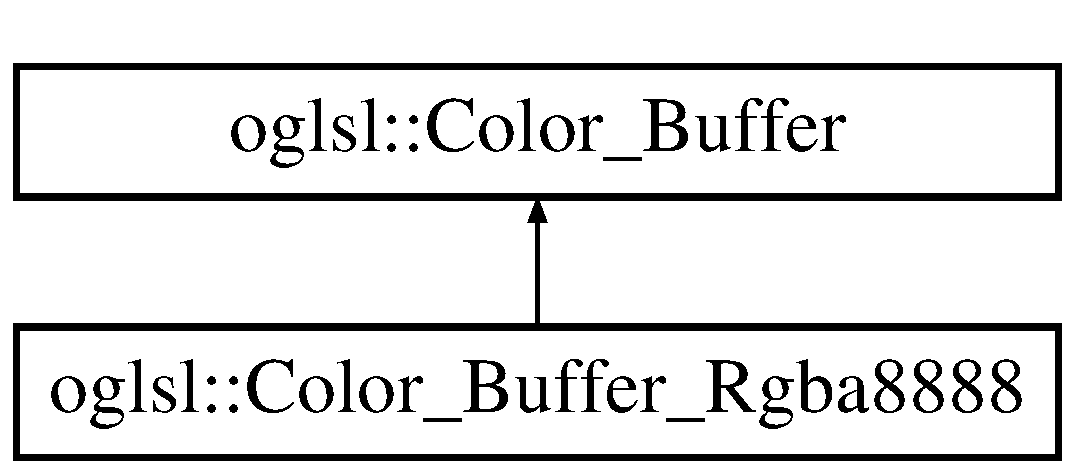
\includegraphics[height=2.000000cm]{classoglsl_1_1_color___buffer}
\end{center}
\end{figure}
\subsection*{Public Member Functions}
\begin{DoxyCompactItemize}
\item 
\mbox{\hyperlink{classoglsl_1_1_color___buffer_aef41961965c6ee31c7948e8d917e9128}{Color\+\_\+\+Buffer}} (size\+\_\+t \mbox{\hyperlink{classoglsl_1_1_color___buffer_a520198eca2cfb64729d134d12efae304}{width}}, size\+\_\+t \mbox{\hyperlink{classoglsl_1_1_color___buffer_a18db6640d6dec54b6695821b9dcaf9c5}{height}})
\item 
size\+\_\+t \mbox{\hyperlink{classoglsl_1_1_color___buffer_ad8f3838322c9e15aa4ebe0f687f0c482}{get\+\_\+width}} () const
\item 
size\+\_\+t \mbox{\hyperlink{classoglsl_1_1_color___buffer_ae13e503d22d65745da0c8c83fb024e5c}{get\+\_\+height}} () const
\item 
int \mbox{\hyperlink{classoglsl_1_1_color___buffer_a0db75521a37e974d14c2b984aabe3c51}{offset\+\_\+at}} (int x, int y) const
\item 
virtual int \mbox{\hyperlink{classoglsl_1_1_color___buffer_a0d182abbbcfddd72467ce085b7eb88b7}{bits\+\_\+per\+\_\+color}} () const =0
\item 
virtual void \mbox{\hyperlink{classoglsl_1_1_color___buffer_a200116c77f9ce43da0156e4260aa1e71}{set\+\_\+color}} (int r, int g, int b)=0
\item 
virtual void \mbox{\hyperlink{classoglsl_1_1_color___buffer_a45662e4f8c5d9776eb125d1c605d36d8}{set\+\_\+pixel}} (int x, int y)=0
\item 
virtual void \mbox{\hyperlink{classoglsl_1_1_color___buffer_aa3b45a2c94da2a9b3e410637152a6a91}{set\+\_\+pixel}} (size\+\_\+t offset)=0
\item 
virtual void \mbox{\hyperlink{classoglsl_1_1_color___buffer_a250795f2a7e3b8edc47accc5605d62a3}{gl\+\_\+draw\+\_\+pixels}} (int raster\+\_\+x, int raster\+\_\+y) const =0
\end{DoxyCompactItemize}
\subsection*{Protected Attributes}
\begin{DoxyCompactItemize}
\item 
size\+\_\+t \mbox{\hyperlink{classoglsl_1_1_color___buffer_a520198eca2cfb64729d134d12efae304}{width}}
\item 
size\+\_\+t \mbox{\hyperlink{classoglsl_1_1_color___buffer_a18db6640d6dec54b6695821b9dcaf9c5}{height}}
\end{DoxyCompactItemize}


\subsection{Constructor \& Destructor Documentation}
\mbox{\Hypertarget{classoglsl_1_1_color___buffer_aef41961965c6ee31c7948e8d917e9128}\label{classoglsl_1_1_color___buffer_aef41961965c6ee31c7948e8d917e9128}} 
\index{oglsl\+::\+Color\+\_\+\+Buffer@{oglsl\+::\+Color\+\_\+\+Buffer}!Color\+\_\+\+Buffer@{Color\+\_\+\+Buffer}}
\index{Color\+\_\+\+Buffer@{Color\+\_\+\+Buffer}!oglsl\+::\+Color\+\_\+\+Buffer@{oglsl\+::\+Color\+\_\+\+Buffer}}
\subsubsection{\texorpdfstring{Color\+\_\+\+Buffer()}{Color\_Buffer()}}
{\footnotesize\ttfamily oglsl\+::\+Color\+\_\+\+Buffer\+::\+Color\+\_\+\+Buffer (\begin{DoxyParamCaption}\item[{size\+\_\+t}]{width,  }\item[{size\+\_\+t}]{height }\end{DoxyParamCaption})\hspace{0.3cm}{\ttfamily [inline]}}



\subsection{Member Function Documentation}
\mbox{\Hypertarget{classoglsl_1_1_color___buffer_a0d182abbbcfddd72467ce085b7eb88b7}\label{classoglsl_1_1_color___buffer_a0d182abbbcfddd72467ce085b7eb88b7}} 
\index{oglsl\+::\+Color\+\_\+\+Buffer@{oglsl\+::\+Color\+\_\+\+Buffer}!bits\+\_\+per\+\_\+color@{bits\+\_\+per\+\_\+color}}
\index{bits\+\_\+per\+\_\+color@{bits\+\_\+per\+\_\+color}!oglsl\+::\+Color\+\_\+\+Buffer@{oglsl\+::\+Color\+\_\+\+Buffer}}
\subsubsection{\texorpdfstring{bits\+\_\+per\+\_\+color()}{bits\_per\_color()}}
{\footnotesize\ttfamily virtual int oglsl\+::\+Color\+\_\+\+Buffer\+::bits\+\_\+per\+\_\+color (\begin{DoxyParamCaption}{ }\end{DoxyParamCaption}) const\hspace{0.3cm}{\ttfamily [pure virtual]}}



Implemented in \mbox{\hyperlink{classoglsl_1_1_color___buffer___rgba8888_a3b4da4899c6765e8689ec2b438ecba84}{oglsl\+::\+Color\+\_\+\+Buffer\+\_\+\+Rgba8888}}.

\mbox{\Hypertarget{classoglsl_1_1_color___buffer_ae13e503d22d65745da0c8c83fb024e5c}\label{classoglsl_1_1_color___buffer_ae13e503d22d65745da0c8c83fb024e5c}} 
\index{oglsl\+::\+Color\+\_\+\+Buffer@{oglsl\+::\+Color\+\_\+\+Buffer}!get\+\_\+height@{get\+\_\+height}}
\index{get\+\_\+height@{get\+\_\+height}!oglsl\+::\+Color\+\_\+\+Buffer@{oglsl\+::\+Color\+\_\+\+Buffer}}
\subsubsection{\texorpdfstring{get\+\_\+height()}{get\_height()}}
{\footnotesize\ttfamily size\+\_\+t oglsl\+::\+Color\+\_\+\+Buffer\+::get\+\_\+height (\begin{DoxyParamCaption}{ }\end{DoxyParamCaption}) const\hspace{0.3cm}{\ttfamily [inline]}}

\mbox{\Hypertarget{classoglsl_1_1_color___buffer_ad8f3838322c9e15aa4ebe0f687f0c482}\label{classoglsl_1_1_color___buffer_ad8f3838322c9e15aa4ebe0f687f0c482}} 
\index{oglsl\+::\+Color\+\_\+\+Buffer@{oglsl\+::\+Color\+\_\+\+Buffer}!get\+\_\+width@{get\+\_\+width}}
\index{get\+\_\+width@{get\+\_\+width}!oglsl\+::\+Color\+\_\+\+Buffer@{oglsl\+::\+Color\+\_\+\+Buffer}}
\subsubsection{\texorpdfstring{get\+\_\+width()}{get\_width()}}
{\footnotesize\ttfamily size\+\_\+t oglsl\+::\+Color\+\_\+\+Buffer\+::get\+\_\+width (\begin{DoxyParamCaption}{ }\end{DoxyParamCaption}) const\hspace{0.3cm}{\ttfamily [inline]}}

\mbox{\Hypertarget{classoglsl_1_1_color___buffer_a250795f2a7e3b8edc47accc5605d62a3}\label{classoglsl_1_1_color___buffer_a250795f2a7e3b8edc47accc5605d62a3}} 
\index{oglsl\+::\+Color\+\_\+\+Buffer@{oglsl\+::\+Color\+\_\+\+Buffer}!gl\+\_\+draw\+\_\+pixels@{gl\+\_\+draw\+\_\+pixels}}
\index{gl\+\_\+draw\+\_\+pixels@{gl\+\_\+draw\+\_\+pixels}!oglsl\+::\+Color\+\_\+\+Buffer@{oglsl\+::\+Color\+\_\+\+Buffer}}
\subsubsection{\texorpdfstring{gl\+\_\+draw\+\_\+pixels()}{gl\_draw\_pixels()}}
{\footnotesize\ttfamily virtual void oglsl\+::\+Color\+\_\+\+Buffer\+::gl\+\_\+draw\+\_\+pixels (\begin{DoxyParamCaption}\item[{int}]{raster\+\_\+x,  }\item[{int}]{raster\+\_\+y }\end{DoxyParamCaption}) const\hspace{0.3cm}{\ttfamily [pure virtual]}}



Implemented in \mbox{\hyperlink{classoglsl_1_1_color___buffer___rgba8888_a06d2384e10162f928e59bfa6e23046da}{oglsl\+::\+Color\+\_\+\+Buffer\+\_\+\+Rgba8888}}.

\mbox{\Hypertarget{classoglsl_1_1_color___buffer_a0db75521a37e974d14c2b984aabe3c51}\label{classoglsl_1_1_color___buffer_a0db75521a37e974d14c2b984aabe3c51}} 
\index{oglsl\+::\+Color\+\_\+\+Buffer@{oglsl\+::\+Color\+\_\+\+Buffer}!offset\+\_\+at@{offset\+\_\+at}}
\index{offset\+\_\+at@{offset\+\_\+at}!oglsl\+::\+Color\+\_\+\+Buffer@{oglsl\+::\+Color\+\_\+\+Buffer}}
\subsubsection{\texorpdfstring{offset\+\_\+at()}{offset\_at()}}
{\footnotesize\ttfamily int oglsl\+::\+Color\+\_\+\+Buffer\+::offset\+\_\+at (\begin{DoxyParamCaption}\item[{int}]{x,  }\item[{int}]{y }\end{DoxyParamCaption}) const\hspace{0.3cm}{\ttfamily [inline]}}

\mbox{\Hypertarget{classoglsl_1_1_color___buffer_a200116c77f9ce43da0156e4260aa1e71}\label{classoglsl_1_1_color___buffer_a200116c77f9ce43da0156e4260aa1e71}} 
\index{oglsl\+::\+Color\+\_\+\+Buffer@{oglsl\+::\+Color\+\_\+\+Buffer}!set\+\_\+color@{set\+\_\+color}}
\index{set\+\_\+color@{set\+\_\+color}!oglsl\+::\+Color\+\_\+\+Buffer@{oglsl\+::\+Color\+\_\+\+Buffer}}
\subsubsection{\texorpdfstring{set\+\_\+color()}{set\_color()}}
{\footnotesize\ttfamily virtual void oglsl\+::\+Color\+\_\+\+Buffer\+::set\+\_\+color (\begin{DoxyParamCaption}\item[{int}]{r,  }\item[{int}]{g,  }\item[{int}]{b }\end{DoxyParamCaption})\hspace{0.3cm}{\ttfamily [pure virtual]}}



Implemented in \mbox{\hyperlink{classoglsl_1_1_color___buffer___rgba8888_a5860a8570962cd69e864e2dc43884373}{oglsl\+::\+Color\+\_\+\+Buffer\+\_\+\+Rgba8888}}.

\mbox{\Hypertarget{classoglsl_1_1_color___buffer_a45662e4f8c5d9776eb125d1c605d36d8}\label{classoglsl_1_1_color___buffer_a45662e4f8c5d9776eb125d1c605d36d8}} 
\index{oglsl\+::\+Color\+\_\+\+Buffer@{oglsl\+::\+Color\+\_\+\+Buffer}!set\+\_\+pixel@{set\+\_\+pixel}}
\index{set\+\_\+pixel@{set\+\_\+pixel}!oglsl\+::\+Color\+\_\+\+Buffer@{oglsl\+::\+Color\+\_\+\+Buffer}}
\subsubsection{\texorpdfstring{set\+\_\+pixel()}{set\_pixel()}\hspace{0.1cm}{\footnotesize\ttfamily [1/2]}}
{\footnotesize\ttfamily virtual void oglsl\+::\+Color\+\_\+\+Buffer\+::set\+\_\+pixel (\begin{DoxyParamCaption}\item[{int}]{x,  }\item[{int}]{y }\end{DoxyParamCaption})\hspace{0.3cm}{\ttfamily [pure virtual]}}



Implemented in \mbox{\hyperlink{classoglsl_1_1_color___buffer___rgba8888_a88a98459049a2366ef58a08a1716b9f9}{oglsl\+::\+Color\+\_\+\+Buffer\+\_\+\+Rgba8888}}.

\mbox{\Hypertarget{classoglsl_1_1_color___buffer_aa3b45a2c94da2a9b3e410637152a6a91}\label{classoglsl_1_1_color___buffer_aa3b45a2c94da2a9b3e410637152a6a91}} 
\index{oglsl\+::\+Color\+\_\+\+Buffer@{oglsl\+::\+Color\+\_\+\+Buffer}!set\+\_\+pixel@{set\+\_\+pixel}}
\index{set\+\_\+pixel@{set\+\_\+pixel}!oglsl\+::\+Color\+\_\+\+Buffer@{oglsl\+::\+Color\+\_\+\+Buffer}}
\subsubsection{\texorpdfstring{set\+\_\+pixel()}{set\_pixel()}\hspace{0.1cm}{\footnotesize\ttfamily [2/2]}}
{\footnotesize\ttfamily virtual void oglsl\+::\+Color\+\_\+\+Buffer\+::set\+\_\+pixel (\begin{DoxyParamCaption}\item[{size\+\_\+t}]{offset }\end{DoxyParamCaption})\hspace{0.3cm}{\ttfamily [pure virtual]}}



Implemented in \mbox{\hyperlink{classoglsl_1_1_color___buffer___rgba8888_a9a62b5f6084af1d6fd1fc7b075c6e025}{oglsl\+::\+Color\+\_\+\+Buffer\+\_\+\+Rgba8888}}.



\subsection{Member Data Documentation}
\mbox{\Hypertarget{classoglsl_1_1_color___buffer_a18db6640d6dec54b6695821b9dcaf9c5}\label{classoglsl_1_1_color___buffer_a18db6640d6dec54b6695821b9dcaf9c5}} 
\index{oglsl\+::\+Color\+\_\+\+Buffer@{oglsl\+::\+Color\+\_\+\+Buffer}!height@{height}}
\index{height@{height}!oglsl\+::\+Color\+\_\+\+Buffer@{oglsl\+::\+Color\+\_\+\+Buffer}}
\subsubsection{\texorpdfstring{height}{height}}
{\footnotesize\ttfamily size\+\_\+t oglsl\+::\+Color\+\_\+\+Buffer\+::height\hspace{0.3cm}{\ttfamily [protected]}}

\mbox{\Hypertarget{classoglsl_1_1_color___buffer_a520198eca2cfb64729d134d12efae304}\label{classoglsl_1_1_color___buffer_a520198eca2cfb64729d134d12efae304}} 
\index{oglsl\+::\+Color\+\_\+\+Buffer@{oglsl\+::\+Color\+\_\+\+Buffer}!width@{width}}
\index{width@{width}!oglsl\+::\+Color\+\_\+\+Buffer@{oglsl\+::\+Color\+\_\+\+Buffer}}
\subsubsection{\texorpdfstring{width}{width}}
{\footnotesize\ttfamily size\+\_\+t oglsl\+::\+Color\+\_\+\+Buffer\+::width\hspace{0.3cm}{\ttfamily [protected]}}



The documentation for this class was generated from the following file\+:\begin{DoxyCompactItemize}
\item 
D\+:/\+Git\+Kraken/3\+D\+Av\+\_\+2/src/\mbox{\hyperlink{_color___buffer_8hpp}{Color\+\_\+\+Buffer.\+hpp}}\end{DoxyCompactItemize}

\hypertarget{classoglsl_1_1_color___buffer___rgba8888}{}\section{oglsl\+:\+:Color\+\_\+\+Buffer\+\_\+\+Rgba8888 Class Reference}
\label{classoglsl_1_1_color___buffer___rgba8888}\index{oglsl\+::\+Color\+\_\+\+Buffer\+\_\+\+Rgba8888@{oglsl\+::\+Color\+\_\+\+Buffer\+\_\+\+Rgba8888}}


{\ttfamily \#include $<$Color\+\_\+\+Buffer\+\_\+\+Rgba8888.\+hpp$>$}

Inheritance diagram for oglsl\+:\+:Color\+\_\+\+Buffer\+\_\+\+Rgba8888\+:\begin{figure}[H]
\begin{center}
\leavevmode
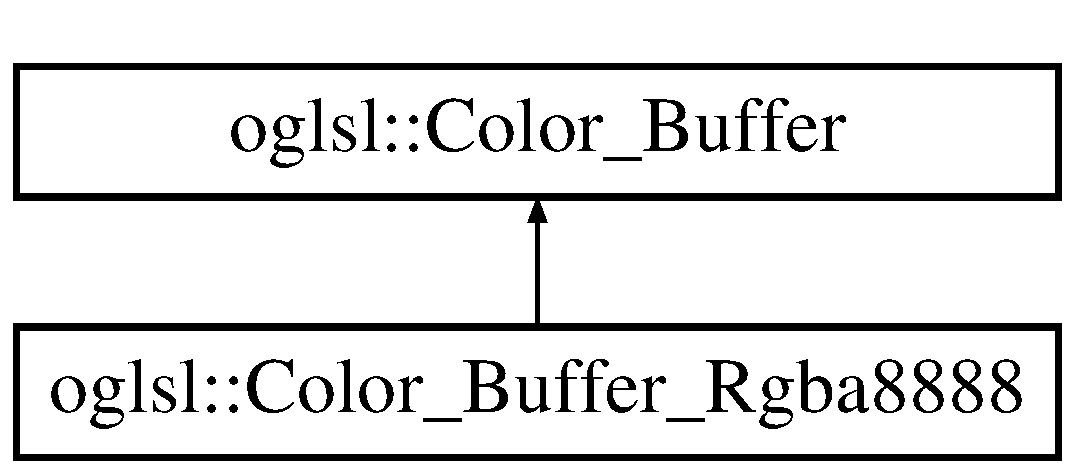
\includegraphics[height=2.000000cm]{classoglsl_1_1_color___buffer___rgba8888}
\end{center}
\end{figure}
\subsection*{Classes}
\begin{DoxyCompactItemize}
\item 
struct \mbox{\hyperlink{structoglsl_1_1_color___buffer___rgba8888_1_1_color}{Color}}
\end{DoxyCompactItemize}
\subsection*{Public Types}
\begin{DoxyCompactItemize}
\item 
typedef std\+::vector$<$ \mbox{\hyperlink{structoglsl_1_1_color___buffer___rgba8888_1_1_color}{Color}} $>$ \mbox{\hyperlink{classoglsl_1_1_color___buffer___rgba8888_a68aacf1d0b3461ed84a7e954ba26936e}{Buffer}}
\end{DoxyCompactItemize}
\subsection*{Public Member Functions}
\begin{DoxyCompactItemize}
\item 
\mbox{\hyperlink{classoglsl_1_1_color___buffer___rgba8888_ac56d38470b2ad20f4ec6d91f92c5b5dd}{Color\+\_\+\+Buffer\+\_\+\+Rgba8888}} (size\+\_\+t \mbox{\hyperlink{classoglsl_1_1_color___buffer_a520198eca2cfb64729d134d12efae304}{width}}, size\+\_\+t \mbox{\hyperlink{classoglsl_1_1_color___buffer_a18db6640d6dec54b6695821b9dcaf9c5}{height}})
\item 
\mbox{\hyperlink{structoglsl_1_1_color___buffer___rgba8888_1_1_color}{Color}} $\ast$ \mbox{\hyperlink{classoglsl_1_1_color___buffer___rgba8888_aa05a3ac094c6af59f348dff1e44d9db3}{colors}} ()
\item 
const \mbox{\hyperlink{structoglsl_1_1_color___buffer___rgba8888_1_1_color}{Color}} $\ast$ \mbox{\hyperlink{classoglsl_1_1_color___buffer___rgba8888_a7261b709b3a0ffe196fe14df5311ba76}{colors}} () const
\item 
int \mbox{\hyperlink{classoglsl_1_1_color___buffer___rgba8888_a3b4da4899c6765e8689ec2b438ecba84}{bits\+\_\+per\+\_\+color}} () const
\item 
size\+\_\+t \mbox{\hyperlink{classoglsl_1_1_color___buffer___rgba8888_a6017d41ebb2a8d35c68e5e2c9efb4c3c}{size}} () const
\item 
void \mbox{\hyperlink{classoglsl_1_1_color___buffer___rgba8888_a5860a8570962cd69e864e2dc43884373}{set\+\_\+color}} (int r, int g, int b)
\item 
void \mbox{\hyperlink{classoglsl_1_1_color___buffer___rgba8888_a54ea503bd5d38f1b669c33d55f47f80e}{set\+\_\+color}} (const \mbox{\hyperlink{structoglsl_1_1_color___buffer___rgba8888_1_1_color}{Color}} \&new\+\_\+color)
\item 
void \mbox{\hyperlink{classoglsl_1_1_color___buffer___rgba8888_a9a62b5f6084af1d6fd1fc7b075c6e025}{set\+\_\+pixel}} (size\+\_\+t offset)
\item 
void \mbox{\hyperlink{classoglsl_1_1_color___buffer___rgba8888_a88a98459049a2366ef58a08a1716b9f9}{set\+\_\+pixel}} (int x, int y)
\item 
uint8\+\_\+t \mbox{\hyperlink{classoglsl_1_1_color___buffer___rgba8888_a0b329444747708cd48509acd56886499}{get\+\_\+pixel}} (int x, int y)
\begin{DoxyCompactList}\small\item\em No terminado. \end{DoxyCompactList}\item 
void \mbox{\hyperlink{classoglsl_1_1_color___buffer___rgba8888_a06d2384e10162f928e59bfa6e23046da}{gl\+\_\+draw\+\_\+pixels}} (int raster\+\_\+x, int raster\+\_\+y) const
\end{DoxyCompactItemize}
\subsection*{Additional Inherited Members}


\subsection{Member Typedef Documentation}
\mbox{\Hypertarget{classoglsl_1_1_color___buffer___rgba8888_a68aacf1d0b3461ed84a7e954ba26936e}\label{classoglsl_1_1_color___buffer___rgba8888_a68aacf1d0b3461ed84a7e954ba26936e}} 
\index{oglsl\+::\+Color\+\_\+\+Buffer\+\_\+\+Rgba8888@{oglsl\+::\+Color\+\_\+\+Buffer\+\_\+\+Rgba8888}!Buffer@{Buffer}}
\index{Buffer@{Buffer}!oglsl\+::\+Color\+\_\+\+Buffer\+\_\+\+Rgba8888@{oglsl\+::\+Color\+\_\+\+Buffer\+\_\+\+Rgba8888}}
\subsubsection{\texorpdfstring{Buffer}{Buffer}}
{\footnotesize\ttfamily typedef std\+::vector$<$ \mbox{\hyperlink{structoglsl_1_1_color___buffer___rgba8888_1_1_color}{Color}} $>$ \mbox{\hyperlink{classoglsl_1_1_color___buffer___rgba8888_a68aacf1d0b3461ed84a7e954ba26936e}{oglsl\+::\+Color\+\_\+\+Buffer\+\_\+\+Rgba8888\+::\+Buffer}}}



\subsection{Constructor \& Destructor Documentation}
\mbox{\Hypertarget{classoglsl_1_1_color___buffer___rgba8888_ac56d38470b2ad20f4ec6d91f92c5b5dd}\label{classoglsl_1_1_color___buffer___rgba8888_ac56d38470b2ad20f4ec6d91f92c5b5dd}} 
\index{oglsl\+::\+Color\+\_\+\+Buffer\+\_\+\+Rgba8888@{oglsl\+::\+Color\+\_\+\+Buffer\+\_\+\+Rgba8888}!Color\+\_\+\+Buffer\+\_\+\+Rgba8888@{Color\+\_\+\+Buffer\+\_\+\+Rgba8888}}
\index{Color\+\_\+\+Buffer\+\_\+\+Rgba8888@{Color\+\_\+\+Buffer\+\_\+\+Rgba8888}!oglsl\+::\+Color\+\_\+\+Buffer\+\_\+\+Rgba8888@{oglsl\+::\+Color\+\_\+\+Buffer\+\_\+\+Rgba8888}}
\subsubsection{\texorpdfstring{Color\+\_\+\+Buffer\+\_\+\+Rgba8888()}{Color\_Buffer\_Rgba8888()}}
{\footnotesize\ttfamily oglsl\+::\+Color\+\_\+\+Buffer\+\_\+\+Rgba8888\+::\+Color\+\_\+\+Buffer\+\_\+\+Rgba8888 (\begin{DoxyParamCaption}\item[{size\+\_\+t}]{width,  }\item[{size\+\_\+t}]{height }\end{DoxyParamCaption})\hspace{0.3cm}{\ttfamily [inline]}}



\subsection{Member Function Documentation}
\mbox{\Hypertarget{classoglsl_1_1_color___buffer___rgba8888_a3b4da4899c6765e8689ec2b438ecba84}\label{classoglsl_1_1_color___buffer___rgba8888_a3b4da4899c6765e8689ec2b438ecba84}} 
\index{oglsl\+::\+Color\+\_\+\+Buffer\+\_\+\+Rgba8888@{oglsl\+::\+Color\+\_\+\+Buffer\+\_\+\+Rgba8888}!bits\+\_\+per\+\_\+color@{bits\+\_\+per\+\_\+color}}
\index{bits\+\_\+per\+\_\+color@{bits\+\_\+per\+\_\+color}!oglsl\+::\+Color\+\_\+\+Buffer\+\_\+\+Rgba8888@{oglsl\+::\+Color\+\_\+\+Buffer\+\_\+\+Rgba8888}}
\subsubsection{\texorpdfstring{bits\+\_\+per\+\_\+color()}{bits\_per\_color()}}
{\footnotesize\ttfamily int oglsl\+::\+Color\+\_\+\+Buffer\+\_\+\+Rgba8888\+::bits\+\_\+per\+\_\+color (\begin{DoxyParamCaption}{ }\end{DoxyParamCaption}) const\hspace{0.3cm}{\ttfamily [inline]}, {\ttfamily [virtual]}}



Implements \mbox{\hyperlink{classoglsl_1_1_color___buffer_a0d182abbbcfddd72467ce085b7eb88b7}{oglsl\+::\+Color\+\_\+\+Buffer}}.

\mbox{\Hypertarget{classoglsl_1_1_color___buffer___rgba8888_aa05a3ac094c6af59f348dff1e44d9db3}\label{classoglsl_1_1_color___buffer___rgba8888_aa05a3ac094c6af59f348dff1e44d9db3}} 
\index{oglsl\+::\+Color\+\_\+\+Buffer\+\_\+\+Rgba8888@{oglsl\+::\+Color\+\_\+\+Buffer\+\_\+\+Rgba8888}!colors@{colors}}
\index{colors@{colors}!oglsl\+::\+Color\+\_\+\+Buffer\+\_\+\+Rgba8888@{oglsl\+::\+Color\+\_\+\+Buffer\+\_\+\+Rgba8888}}
\subsubsection{\texorpdfstring{colors()}{colors()}\hspace{0.1cm}{\footnotesize\ttfamily [1/2]}}
{\footnotesize\ttfamily \mbox{\hyperlink{structoglsl_1_1_color___buffer___rgba8888_1_1_color}{Color}}$\ast$ oglsl\+::\+Color\+\_\+\+Buffer\+\_\+\+Rgba8888\+::colors (\begin{DoxyParamCaption}{ }\end{DoxyParamCaption})\hspace{0.3cm}{\ttfamily [inline]}}

\mbox{\Hypertarget{classoglsl_1_1_color___buffer___rgba8888_a7261b709b3a0ffe196fe14df5311ba76}\label{classoglsl_1_1_color___buffer___rgba8888_a7261b709b3a0ffe196fe14df5311ba76}} 
\index{oglsl\+::\+Color\+\_\+\+Buffer\+\_\+\+Rgba8888@{oglsl\+::\+Color\+\_\+\+Buffer\+\_\+\+Rgba8888}!colors@{colors}}
\index{colors@{colors}!oglsl\+::\+Color\+\_\+\+Buffer\+\_\+\+Rgba8888@{oglsl\+::\+Color\+\_\+\+Buffer\+\_\+\+Rgba8888}}
\subsubsection{\texorpdfstring{colors()}{colors()}\hspace{0.1cm}{\footnotesize\ttfamily [2/2]}}
{\footnotesize\ttfamily const \mbox{\hyperlink{structoglsl_1_1_color___buffer___rgba8888_1_1_color}{Color}}$\ast$ oglsl\+::\+Color\+\_\+\+Buffer\+\_\+\+Rgba8888\+::colors (\begin{DoxyParamCaption}{ }\end{DoxyParamCaption}) const\hspace{0.3cm}{\ttfamily [inline]}}

\mbox{\Hypertarget{classoglsl_1_1_color___buffer___rgba8888_a0b329444747708cd48509acd56886499}\label{classoglsl_1_1_color___buffer___rgba8888_a0b329444747708cd48509acd56886499}} 
\index{oglsl\+::\+Color\+\_\+\+Buffer\+\_\+\+Rgba8888@{oglsl\+::\+Color\+\_\+\+Buffer\+\_\+\+Rgba8888}!get\+\_\+pixel@{get\+\_\+pixel}}
\index{get\+\_\+pixel@{get\+\_\+pixel}!oglsl\+::\+Color\+\_\+\+Buffer\+\_\+\+Rgba8888@{oglsl\+::\+Color\+\_\+\+Buffer\+\_\+\+Rgba8888}}
\subsubsection{\texorpdfstring{get\+\_\+pixel()}{get\_pixel()}}
{\footnotesize\ttfamily uint8\+\_\+t oglsl\+::\+Color\+\_\+\+Buffer\+\_\+\+Rgba8888\+::get\+\_\+pixel (\begin{DoxyParamCaption}\item[{int}]{x,  }\item[{int}]{y }\end{DoxyParamCaption})\hspace{0.3cm}{\ttfamily [inline]}}



No terminado. 

\mbox{\Hypertarget{classoglsl_1_1_color___buffer___rgba8888_a06d2384e10162f928e59bfa6e23046da}\label{classoglsl_1_1_color___buffer___rgba8888_a06d2384e10162f928e59bfa6e23046da}} 
\index{oglsl\+::\+Color\+\_\+\+Buffer\+\_\+\+Rgba8888@{oglsl\+::\+Color\+\_\+\+Buffer\+\_\+\+Rgba8888}!gl\+\_\+draw\+\_\+pixels@{gl\+\_\+draw\+\_\+pixels}}
\index{gl\+\_\+draw\+\_\+pixels@{gl\+\_\+draw\+\_\+pixels}!oglsl\+::\+Color\+\_\+\+Buffer\+\_\+\+Rgba8888@{oglsl\+::\+Color\+\_\+\+Buffer\+\_\+\+Rgba8888}}
\subsubsection{\texorpdfstring{gl\+\_\+draw\+\_\+pixels()}{gl\_draw\_pixels()}}
{\footnotesize\ttfamily void oglsl\+::\+Color\+\_\+\+Buffer\+\_\+\+Rgba8888\+::gl\+\_\+draw\+\_\+pixels (\begin{DoxyParamCaption}\item[{int}]{raster\+\_\+x,  }\item[{int}]{raster\+\_\+y }\end{DoxyParamCaption}) const\hspace{0.3cm}{\ttfamily [inline]}, {\ttfamily [virtual]}}



Implements \mbox{\hyperlink{classoglsl_1_1_color___buffer_a250795f2a7e3b8edc47accc5605d62a3}{oglsl\+::\+Color\+\_\+\+Buffer}}.

\mbox{\Hypertarget{classoglsl_1_1_color___buffer___rgba8888_a5860a8570962cd69e864e2dc43884373}\label{classoglsl_1_1_color___buffer___rgba8888_a5860a8570962cd69e864e2dc43884373}} 
\index{oglsl\+::\+Color\+\_\+\+Buffer\+\_\+\+Rgba8888@{oglsl\+::\+Color\+\_\+\+Buffer\+\_\+\+Rgba8888}!set\+\_\+color@{set\+\_\+color}}
\index{set\+\_\+color@{set\+\_\+color}!oglsl\+::\+Color\+\_\+\+Buffer\+\_\+\+Rgba8888@{oglsl\+::\+Color\+\_\+\+Buffer\+\_\+\+Rgba8888}}
\subsubsection{\texorpdfstring{set\+\_\+color()}{set\_color()}\hspace{0.1cm}{\footnotesize\ttfamily [1/2]}}
{\footnotesize\ttfamily void oglsl\+::\+Color\+\_\+\+Buffer\+\_\+\+Rgba8888\+::set\+\_\+color (\begin{DoxyParamCaption}\item[{int}]{r,  }\item[{int}]{g,  }\item[{int}]{b }\end{DoxyParamCaption})\hspace{0.3cm}{\ttfamily [inline]}, {\ttfamily [virtual]}}



Implements \mbox{\hyperlink{classoglsl_1_1_color___buffer_a200116c77f9ce43da0156e4260aa1e71}{oglsl\+::\+Color\+\_\+\+Buffer}}.

\mbox{\Hypertarget{classoglsl_1_1_color___buffer___rgba8888_a54ea503bd5d38f1b669c33d55f47f80e}\label{classoglsl_1_1_color___buffer___rgba8888_a54ea503bd5d38f1b669c33d55f47f80e}} 
\index{oglsl\+::\+Color\+\_\+\+Buffer\+\_\+\+Rgba8888@{oglsl\+::\+Color\+\_\+\+Buffer\+\_\+\+Rgba8888}!set\+\_\+color@{set\+\_\+color}}
\index{set\+\_\+color@{set\+\_\+color}!oglsl\+::\+Color\+\_\+\+Buffer\+\_\+\+Rgba8888@{oglsl\+::\+Color\+\_\+\+Buffer\+\_\+\+Rgba8888}}
\subsubsection{\texorpdfstring{set\+\_\+color()}{set\_color()}\hspace{0.1cm}{\footnotesize\ttfamily [2/2]}}
{\footnotesize\ttfamily void oglsl\+::\+Color\+\_\+\+Buffer\+\_\+\+Rgba8888\+::set\+\_\+color (\begin{DoxyParamCaption}\item[{const \mbox{\hyperlink{structoglsl_1_1_color___buffer___rgba8888_1_1_color}{Color}} \&}]{new\+\_\+color }\end{DoxyParamCaption})\hspace{0.3cm}{\ttfamily [inline]}}

\mbox{\Hypertarget{classoglsl_1_1_color___buffer___rgba8888_a9a62b5f6084af1d6fd1fc7b075c6e025}\label{classoglsl_1_1_color___buffer___rgba8888_a9a62b5f6084af1d6fd1fc7b075c6e025}} 
\index{oglsl\+::\+Color\+\_\+\+Buffer\+\_\+\+Rgba8888@{oglsl\+::\+Color\+\_\+\+Buffer\+\_\+\+Rgba8888}!set\+\_\+pixel@{set\+\_\+pixel}}
\index{set\+\_\+pixel@{set\+\_\+pixel}!oglsl\+::\+Color\+\_\+\+Buffer\+\_\+\+Rgba8888@{oglsl\+::\+Color\+\_\+\+Buffer\+\_\+\+Rgba8888}}
\subsubsection{\texorpdfstring{set\+\_\+pixel()}{set\_pixel()}\hspace{0.1cm}{\footnotesize\ttfamily [1/2]}}
{\footnotesize\ttfamily void oglsl\+::\+Color\+\_\+\+Buffer\+\_\+\+Rgba8888\+::set\+\_\+pixel (\begin{DoxyParamCaption}\item[{size\+\_\+t}]{offset }\end{DoxyParamCaption})\hspace{0.3cm}{\ttfamily [inline]}, {\ttfamily [virtual]}}



Implements \mbox{\hyperlink{classoglsl_1_1_color___buffer_aa3b45a2c94da2a9b3e410637152a6a91}{oglsl\+::\+Color\+\_\+\+Buffer}}.

\mbox{\Hypertarget{classoglsl_1_1_color___buffer___rgba8888_a88a98459049a2366ef58a08a1716b9f9}\label{classoglsl_1_1_color___buffer___rgba8888_a88a98459049a2366ef58a08a1716b9f9}} 
\index{oglsl\+::\+Color\+\_\+\+Buffer\+\_\+\+Rgba8888@{oglsl\+::\+Color\+\_\+\+Buffer\+\_\+\+Rgba8888}!set\+\_\+pixel@{set\+\_\+pixel}}
\index{set\+\_\+pixel@{set\+\_\+pixel}!oglsl\+::\+Color\+\_\+\+Buffer\+\_\+\+Rgba8888@{oglsl\+::\+Color\+\_\+\+Buffer\+\_\+\+Rgba8888}}
\subsubsection{\texorpdfstring{set\+\_\+pixel()}{set\_pixel()}\hspace{0.1cm}{\footnotesize\ttfamily [2/2]}}
{\footnotesize\ttfamily void oglsl\+::\+Color\+\_\+\+Buffer\+\_\+\+Rgba8888\+::set\+\_\+pixel (\begin{DoxyParamCaption}\item[{int}]{x,  }\item[{int}]{y }\end{DoxyParamCaption})\hspace{0.3cm}{\ttfamily [inline]}, {\ttfamily [virtual]}}



Implements \mbox{\hyperlink{classoglsl_1_1_color___buffer_a45662e4f8c5d9776eb125d1c605d36d8}{oglsl\+::\+Color\+\_\+\+Buffer}}.

\mbox{\Hypertarget{classoglsl_1_1_color___buffer___rgba8888_a6017d41ebb2a8d35c68e5e2c9efb4c3c}\label{classoglsl_1_1_color___buffer___rgba8888_a6017d41ebb2a8d35c68e5e2c9efb4c3c}} 
\index{oglsl\+::\+Color\+\_\+\+Buffer\+\_\+\+Rgba8888@{oglsl\+::\+Color\+\_\+\+Buffer\+\_\+\+Rgba8888}!size@{size}}
\index{size@{size}!oglsl\+::\+Color\+\_\+\+Buffer\+\_\+\+Rgba8888@{oglsl\+::\+Color\+\_\+\+Buffer\+\_\+\+Rgba8888}}
\subsubsection{\texorpdfstring{size()}{size()}}
{\footnotesize\ttfamily size\+\_\+t oglsl\+::\+Color\+\_\+\+Buffer\+\_\+\+Rgba8888\+::size (\begin{DoxyParamCaption}{ }\end{DoxyParamCaption}) const\hspace{0.3cm}{\ttfamily [inline]}}



The documentation for this class was generated from the following file\+:\begin{DoxyCompactItemize}
\item 
D\+:/\+Git\+Kraken/3\+D\+Av\+\_\+2/src/\mbox{\hyperlink{_color___buffer___rgba8888_8hpp}{Color\+\_\+\+Buffer\+\_\+\+Rgba8888.\+hpp}}\end{DoxyCompactItemize}

\hypertarget{classoglsl_1_1_cube}{}\section{oglsl\+:\+:Cube Class Reference}
\label{classoglsl_1_1_cube}\index{oglsl\+::\+Cube@{oglsl\+::\+Cube}}


{\ttfamily \#include $<$Cube.\+hpp$>$}

\subsection*{Public Member Functions}
\begin{DoxyCompactItemize}
\item 
\mbox{\hyperlink{classoglsl_1_1_cube_a3be7fbbad6d33b8ca68487fea7e20bdf}{Cube}} ()
\item 
\mbox{\hyperlink{classoglsl_1_1_cube_ab82f621c8aeb1ce7ccd72afd605d6b7a}{$\sim$\+Cube}} ()
\item 
void \mbox{\hyperlink{classoglsl_1_1_cube_a9f968872ab6a7ee0362e49a0c5f4e8b6}{render}} ()
\end{DoxyCompactItemize}


\subsection{Constructor \& Destructor Documentation}
\mbox{\Hypertarget{classoglsl_1_1_cube_a3be7fbbad6d33b8ca68487fea7e20bdf}\label{classoglsl_1_1_cube_a3be7fbbad6d33b8ca68487fea7e20bdf}} 
\index{oglsl\+::\+Cube@{oglsl\+::\+Cube}!Cube@{Cube}}
\index{Cube@{Cube}!oglsl\+::\+Cube@{oglsl\+::\+Cube}}
\subsubsection{\texorpdfstring{Cube()}{Cube()}}
{\footnotesize\ttfamily example\+::\+Cube\+::\+Cube (\begin{DoxyParamCaption}{ }\end{DoxyParamCaption})}

\mbox{\Hypertarget{classoglsl_1_1_cube_ab82f621c8aeb1ce7ccd72afd605d6b7a}\label{classoglsl_1_1_cube_ab82f621c8aeb1ce7ccd72afd605d6b7a}} 
\index{oglsl\+::\+Cube@{oglsl\+::\+Cube}!````~Cube@{$\sim$\+Cube}}
\index{````~Cube@{$\sim$\+Cube}!oglsl\+::\+Cube@{oglsl\+::\+Cube}}
\subsubsection{\texorpdfstring{$\sim$\+Cube()}{~Cube()}}
{\footnotesize\ttfamily example\+::\+Cube\+::$\sim$\+Cube (\begin{DoxyParamCaption}{ }\end{DoxyParamCaption})}



\subsection{Member Function Documentation}
\mbox{\Hypertarget{classoglsl_1_1_cube_a9f968872ab6a7ee0362e49a0c5f4e8b6}\label{classoglsl_1_1_cube_a9f968872ab6a7ee0362e49a0c5f4e8b6}} 
\index{oglsl\+::\+Cube@{oglsl\+::\+Cube}!render@{render}}
\index{render@{render}!oglsl\+::\+Cube@{oglsl\+::\+Cube}}
\subsubsection{\texorpdfstring{render()}{render()}}
{\footnotesize\ttfamily void example\+::\+Cube\+::render (\begin{DoxyParamCaption}{ }\end{DoxyParamCaption})}



The documentation for this class was generated from the following files\+:\begin{DoxyCompactItemize}
\item 
D\+:/\+Git\+Kraken/3\+D\+Av\+\_\+2/src/\mbox{\hyperlink{_cube_8hpp}{Cube.\+hpp}}\item 
D\+:/\+Git\+Kraken/3\+D\+Av\+\_\+2/src/\mbox{\hyperlink{_cube_8cpp}{Cube.\+cpp}}\end{DoxyCompactItemize}

\hypertarget{classoglsl_1_1_elevation___mesh}{}\section{oglsl\+:\+:Elevation\+\_\+\+Mesh Class Reference}
\label{classoglsl_1_1_elevation___mesh}\index{oglsl\+::\+Elevation\+\_\+\+Mesh@{oglsl\+::\+Elevation\+\_\+\+Mesh}}


Represents a terrain mesh created from an elevation texture.  




{\ttfamily \#include $<$Elevation\+\_\+\+Mesh.\+hpp$>$}

Inheritance diagram for oglsl\+:\+:Elevation\+\_\+\+Mesh\+:\begin{figure}[H]
\begin{center}
\leavevmode
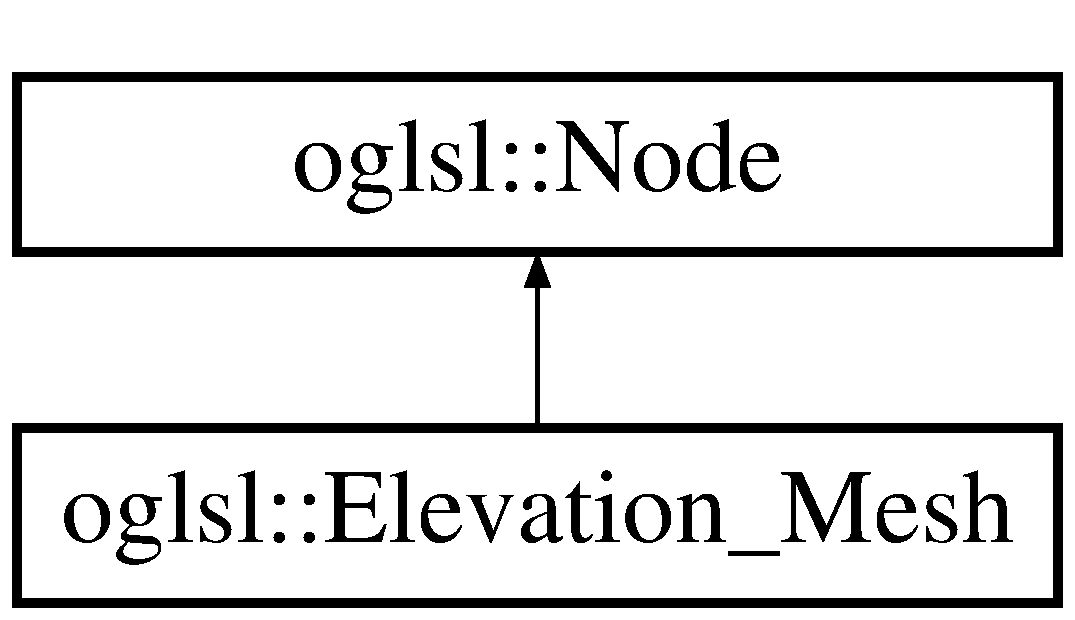
\includegraphics[height=2.000000cm]{classoglsl_1_1_elevation___mesh}
\end{center}
\end{figure}
\subsection*{Public Member Functions}
\begin{DoxyCompactItemize}
\item 
\mbox{\hyperlink{classoglsl_1_1_elevation___mesh_ab23733c3bcec54943bb012c272a44ca3}{Elevation\+\_\+\+Mesh}} (int cols, int rows, float width, float depth, float elevation, shared\+\_\+ptr$<$ \mbox{\hyperlink{classoglsl_1_1_shader___program}{Shader\+\_\+\+Program}} $>$ shader)
\begin{DoxyCompactList}\small\item\em Creates an elevetion mesh with texture. \end{DoxyCompactList}\item 
\mbox{\hyperlink{classoglsl_1_1_elevation___mesh_afc3f5227d96a854e9e66723fbf728cb2}{$\sim$\+Elevation\+\_\+\+Mesh}} ()
\item 
glm\+::vec3 \mbox{\hyperlink{classoglsl_1_1_elevation___mesh_ad141ee161715d896f41ca7b31b9d0c7d}{calculate\+\_\+normal}} (const Point3f \&p0, const Point3f \&p1, const Point3f \&p2)
\item 
glm\+::vec3 \mbox{\hyperlink{classoglsl_1_1_elevation___mesh_a768320a6bdacdeff34528c0c08f92b5c}{calculate\+\_\+normal}} (const Point3f \&p0, const Point3f \&p1, const Point3f \&p2, const Point3f \&p3, const Point3f \&p4, const Point3f \&p5, const Point3f \&p6, const Point3f \&p7, const Point3f \&p8)
\item 
void \mbox{\hyperlink{classoglsl_1_1_elevation___mesh_afb39dc1633680dccabb4b8da72ac4733}{render}} (const glm\+::mat4 \&parent\+\_\+model\+\_\+view) override
\begin{DoxyCompactList}\small\item\em Renders the mesh. \end{DoxyCompactList}\end{DoxyCompactItemize}
\subsection*{Additional Inherited Members}


\subsection{Detailed Description}
Represents a terrain mesh created from an elevation texture. 

The texture works in B/W scale or red scale. 

\subsection{Constructor \& Destructor Documentation}
\mbox{\Hypertarget{classoglsl_1_1_elevation___mesh_ab23733c3bcec54943bb012c272a44ca3}\label{classoglsl_1_1_elevation___mesh_ab23733c3bcec54943bb012c272a44ca3}} 
\index{oglsl\+::\+Elevation\+\_\+\+Mesh@{oglsl\+::\+Elevation\+\_\+\+Mesh}!Elevation\+\_\+\+Mesh@{Elevation\+\_\+\+Mesh}}
\index{Elevation\+\_\+\+Mesh@{Elevation\+\_\+\+Mesh}!oglsl\+::\+Elevation\+\_\+\+Mesh@{oglsl\+::\+Elevation\+\_\+\+Mesh}}
\subsubsection{\texorpdfstring{Elevation\+\_\+\+Mesh()}{Elevation\_Mesh()}}
{\footnotesize\ttfamily oglsl\+::\+Elevation\+\_\+\+Mesh\+::\+Elevation\+\_\+\+Mesh (\begin{DoxyParamCaption}\item[{int}]{cols,  }\item[{int}]{rows,  }\item[{float}]{width,  }\item[{float}]{depth,  }\item[{float}]{elevation,  }\item[{shared\+\_\+ptr$<$ \mbox{\hyperlink{classoglsl_1_1_shader___program}{Shader\+\_\+\+Program}} $>$}]{shader }\end{DoxyParamCaption})}



Creates an elevetion mesh with texture. 

\mbox{\Hypertarget{classoglsl_1_1_elevation___mesh_afc3f5227d96a854e9e66723fbf728cb2}\label{classoglsl_1_1_elevation___mesh_afc3f5227d96a854e9e66723fbf728cb2}} 
\index{oglsl\+::\+Elevation\+\_\+\+Mesh@{oglsl\+::\+Elevation\+\_\+\+Mesh}!````~Elevation\+\_\+\+Mesh@{$\sim$\+Elevation\+\_\+\+Mesh}}
\index{````~Elevation\+\_\+\+Mesh@{$\sim$\+Elevation\+\_\+\+Mesh}!oglsl\+::\+Elevation\+\_\+\+Mesh@{oglsl\+::\+Elevation\+\_\+\+Mesh}}
\subsubsection{\texorpdfstring{$\sim$\+Elevation\+\_\+\+Mesh()}{~Elevation\_Mesh()}}
{\footnotesize\ttfamily oglsl\+::\+Elevation\+\_\+\+Mesh\+::$\sim$\+Elevation\+\_\+\+Mesh (\begin{DoxyParamCaption}{ }\end{DoxyParamCaption})}



\subsection{Member Function Documentation}
\mbox{\Hypertarget{classoglsl_1_1_elevation___mesh_ad141ee161715d896f41ca7b31b9d0c7d}\label{classoglsl_1_1_elevation___mesh_ad141ee161715d896f41ca7b31b9d0c7d}} 
\index{oglsl\+::\+Elevation\+\_\+\+Mesh@{oglsl\+::\+Elevation\+\_\+\+Mesh}!calculate\+\_\+normal@{calculate\+\_\+normal}}
\index{calculate\+\_\+normal@{calculate\+\_\+normal}!oglsl\+::\+Elevation\+\_\+\+Mesh@{oglsl\+::\+Elevation\+\_\+\+Mesh}}
\subsubsection{\texorpdfstring{calculate\+\_\+normal()}{calculate\_normal()}\hspace{0.1cm}{\footnotesize\ttfamily [1/2]}}
{\footnotesize\ttfamily glm\+::vec3 oglsl\+::\+Elevation\+\_\+\+Mesh\+::calculate\+\_\+normal (\begin{DoxyParamCaption}\item[{const Point3f \&}]{p0,  }\item[{const Point3f \&}]{p1,  }\item[{const Point3f \&}]{p2 }\end{DoxyParamCaption})}

\mbox{\Hypertarget{classoglsl_1_1_elevation___mesh_a768320a6bdacdeff34528c0c08f92b5c}\label{classoglsl_1_1_elevation___mesh_a768320a6bdacdeff34528c0c08f92b5c}} 
\index{oglsl\+::\+Elevation\+\_\+\+Mesh@{oglsl\+::\+Elevation\+\_\+\+Mesh}!calculate\+\_\+normal@{calculate\+\_\+normal}}
\index{calculate\+\_\+normal@{calculate\+\_\+normal}!oglsl\+::\+Elevation\+\_\+\+Mesh@{oglsl\+::\+Elevation\+\_\+\+Mesh}}
\subsubsection{\texorpdfstring{calculate\+\_\+normal()}{calculate\_normal()}\hspace{0.1cm}{\footnotesize\ttfamily [2/2]}}
{\footnotesize\ttfamily glm\+::vec3 oglsl\+::\+Elevation\+\_\+\+Mesh\+::calculate\+\_\+normal (\begin{DoxyParamCaption}\item[{const Point3f \&}]{p0,  }\item[{const Point3f \&}]{p1,  }\item[{const Point3f \&}]{p2,  }\item[{const Point3f \&}]{p3,  }\item[{const Point3f \&}]{p4,  }\item[{const Point3f \&}]{p5,  }\item[{const Point3f \&}]{p6,  }\item[{const Point3f \&}]{p7,  }\item[{const Point3f \&}]{p8 }\end{DoxyParamCaption})}

\mbox{\Hypertarget{classoglsl_1_1_elevation___mesh_afb39dc1633680dccabb4b8da72ac4733}\label{classoglsl_1_1_elevation___mesh_afb39dc1633680dccabb4b8da72ac4733}} 
\index{oglsl\+::\+Elevation\+\_\+\+Mesh@{oglsl\+::\+Elevation\+\_\+\+Mesh}!render@{render}}
\index{render@{render}!oglsl\+::\+Elevation\+\_\+\+Mesh@{oglsl\+::\+Elevation\+\_\+\+Mesh}}
\subsubsection{\texorpdfstring{render()}{render()}}
{\footnotesize\ttfamily void oglsl\+::\+Elevation\+\_\+\+Mesh\+::render (\begin{DoxyParamCaption}\item[{const glm\+::mat4 \&}]{parent\+\_\+model\+\_\+view }\end{DoxyParamCaption})\hspace{0.3cm}{\ttfamily [override]}, {\ttfamily [virtual]}}



Renders the mesh. 



Reimplemented from \mbox{\hyperlink{classoglsl_1_1_node_a09545b18a2d798327601a6251c091444}{oglsl\+::\+Node}}.



The documentation for this class was generated from the following files\+:\begin{DoxyCompactItemize}
\item 
D\+:/\+Git\+Kraken/3\+D\+Av\+\_\+2/src/\mbox{\hyperlink{_elevation___mesh_8hpp}{Elevation\+\_\+\+Mesh.\+hpp}}\item 
D\+:/\+Git\+Kraken/3\+D\+Av\+\_\+2/src/\mbox{\hyperlink{_elevation___mesh_8cpp}{Elevation\+\_\+\+Mesh.\+cpp}}\end{DoxyCompactItemize}

\hypertarget{classoglsl_1_1_fragment___shader}{}\section{oglsl\+:\+:Fragment\+\_\+\+Shader Class Reference}
\label{classoglsl_1_1_fragment___shader}\index{oglsl\+::\+Fragment\+\_\+\+Shader@{oglsl\+::\+Fragment\+\_\+\+Shader}}


{\ttfamily \#include $<$Fragment\+\_\+\+Shader.\+hpp$>$}

Inheritance diagram for oglsl\+:\+:Fragment\+\_\+\+Shader\+:\begin{figure}[H]
\begin{center}
\leavevmode
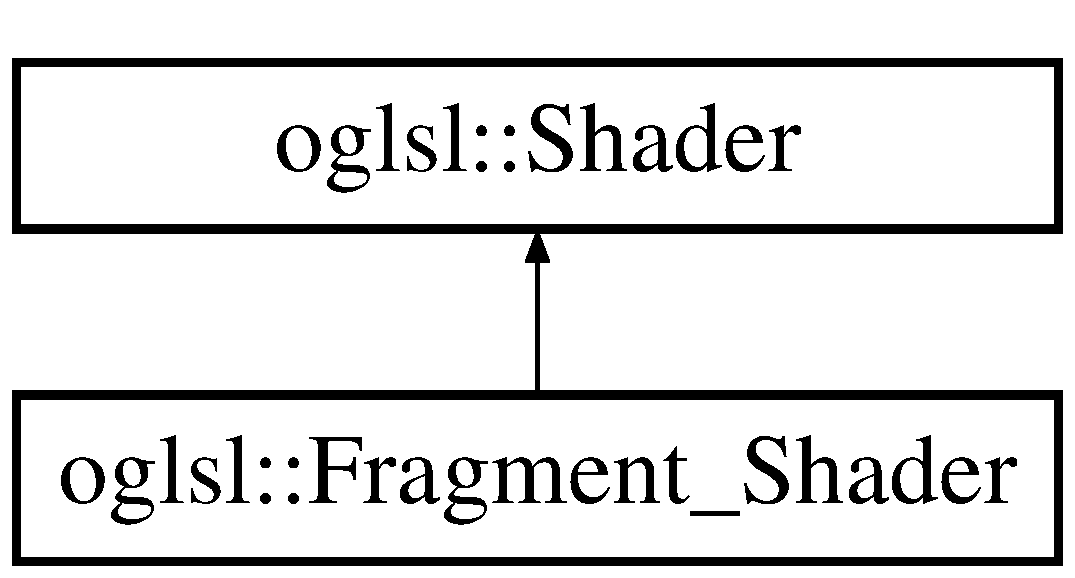
\includegraphics[height=2.000000cm]{classoglsl_1_1_fragment___shader}
\end{center}
\end{figure}
\subsection*{Public Member Functions}
\begin{DoxyCompactItemize}
\item 
\mbox{\hyperlink{classoglsl_1_1_fragment___shader_a69700cf85e0a653b0de60f3694886f4f}{Fragment\+\_\+\+Shader}} (const \mbox{\hyperlink{classoglsl_1_1_shader_1_1_source___code}{Source\+\_\+\+Code}} \&source\+\_\+code)
\end{DoxyCompactItemize}
\subsection*{Additional Inherited Members}


\subsection{Constructor \& Destructor Documentation}
\mbox{\Hypertarget{classoglsl_1_1_fragment___shader_a69700cf85e0a653b0de60f3694886f4f}\label{classoglsl_1_1_fragment___shader_a69700cf85e0a653b0de60f3694886f4f}} 
\index{oglsl\+::\+Fragment\+\_\+\+Shader@{oglsl\+::\+Fragment\+\_\+\+Shader}!Fragment\+\_\+\+Shader@{Fragment\+\_\+\+Shader}}
\index{Fragment\+\_\+\+Shader@{Fragment\+\_\+\+Shader}!oglsl\+::\+Fragment\+\_\+\+Shader@{oglsl\+::\+Fragment\+\_\+\+Shader}}
\subsubsection{\texorpdfstring{Fragment\+\_\+\+Shader()}{Fragment\_Shader()}}
{\footnotesize\ttfamily oglsl\+::\+Fragment\+\_\+\+Shader\+::\+Fragment\+\_\+\+Shader (\begin{DoxyParamCaption}\item[{const \mbox{\hyperlink{classoglsl_1_1_shader_1_1_source___code}{Source\+\_\+\+Code}} \&}]{source\+\_\+code }\end{DoxyParamCaption})\hspace{0.3cm}{\ttfamily [inline]}}



The documentation for this class was generated from the following file\+:\begin{DoxyCompactItemize}
\item 
D\+:/\+Git\+Kraken/3\+D\+Av\+\_\+2/src/\mbox{\hyperlink{_fragment___shader_8hpp}{Fragment\+\_\+\+Shader.\+hpp}}\end{DoxyCompactItemize}

\hypertarget{classoglsl_1_1_framebuffer}{}\section{oglsl\+:\+:Framebuffer Class Reference}
\label{classoglsl_1_1_framebuffer}\index{oglsl\+::\+Framebuffer@{oglsl\+::\+Framebuffer}}


Used to render the scene to a framebuffer and apply post processig shaders to it.  




{\ttfamily \#include $<$Framebuffer.\+hpp$>$}

\subsection*{Public Member Functions}
\begin{DoxyCompactItemize}
\item 
\mbox{\hyperlink{classoglsl_1_1_framebuffer_a69506454416fe0134814dade467e147e}{Framebuffer}} (std\+::shared\+\_\+ptr$<$ \mbox{\hyperlink{classoglsl_1_1_shader___program}{Shader\+\_\+\+Program}} $>$ shader)
\begin{DoxyCompactList}\small\item\em Creates a \mbox{\hyperlink{classoglsl_1_1_framebuffer}{Framebuffer}}. \end{DoxyCompactList}\item 
void \mbox{\hyperlink{classoglsl_1_1_framebuffer_a628dd0fb23006b139c75786a3d7da1a6}{render}} (int width, int height)
\begin{DoxyCompactList}\small\item\em Renders the framebuffer in the specified screen dymensions. \end{DoxyCompactList}\item 
void \mbox{\hyperlink{classoglsl_1_1_framebuffer_a3e0f4248aed96f483a318b34ea8c9cb8}{set\+Framebuffer}} ()
\begin{DoxyCompactList}\small\item\em Inits the gl\+Viewport and the G\+L\+\_\+\+F\+R\+A\+M\+E\+B\+U\+F\+F\+ER for the scene objects to be rendered. \end{DoxyCompactList}\end{DoxyCompactItemize}


\subsection{Detailed Description}
Used to render the scene to a framebuffer and apply post processig shaders to it. 

\subsection{Constructor \& Destructor Documentation}
\mbox{\Hypertarget{classoglsl_1_1_framebuffer_a69506454416fe0134814dade467e147e}\label{classoglsl_1_1_framebuffer_a69506454416fe0134814dade467e147e}} 
\index{oglsl\+::\+Framebuffer@{oglsl\+::\+Framebuffer}!Framebuffer@{Framebuffer}}
\index{Framebuffer@{Framebuffer}!oglsl\+::\+Framebuffer@{oglsl\+::\+Framebuffer}}
\subsubsection{\texorpdfstring{Framebuffer()}{Framebuffer()}}
{\footnotesize\ttfamily oglsl\+::\+Framebuffer\+::\+Framebuffer (\begin{DoxyParamCaption}\item[{std\+::shared\+\_\+ptr$<$ \mbox{\hyperlink{classoglsl_1_1_shader___program}{Shader\+\_\+\+Program}} $>$}]{shader }\end{DoxyParamCaption})}



Creates a \mbox{\hyperlink{classoglsl_1_1_framebuffer}{Framebuffer}}. 

Creation of the G\+L\+\_\+\+F\+R\+A\+M\+E\+B\+U\+F\+F\+ER, texture, z-\/buffer and the screen quad. 
\begin{DoxyParams}{Parameters}
{\em post} & processing shader that will be used to render the framebuffer. \\
\hline
\end{DoxyParams}


\subsection{Member Function Documentation}
\mbox{\Hypertarget{classoglsl_1_1_framebuffer_a628dd0fb23006b139c75786a3d7da1a6}\label{classoglsl_1_1_framebuffer_a628dd0fb23006b139c75786a3d7da1a6}} 
\index{oglsl\+::\+Framebuffer@{oglsl\+::\+Framebuffer}!render@{render}}
\index{render@{render}!oglsl\+::\+Framebuffer@{oglsl\+::\+Framebuffer}}
\subsubsection{\texorpdfstring{render()}{render()}}
{\footnotesize\ttfamily void oglsl\+::\+Framebuffer\+::render (\begin{DoxyParamCaption}\item[{int}]{width,  }\item[{int}]{height }\end{DoxyParamCaption})}



Renders the framebuffer in the specified screen dymensions. 

The framebuffer needs to be set before calling to render. To be called after rendering all other scene elements. 
\begin{DoxyParams}{Parameters}
{\em width} & screen width. \\
\hline
{\em height} & screen height. \\
\hline
\end{DoxyParams}
\mbox{\Hypertarget{classoglsl_1_1_framebuffer_a3e0f4248aed96f483a318b34ea8c9cb8}\label{classoglsl_1_1_framebuffer_a3e0f4248aed96f483a318b34ea8c9cb8}} 
\index{oglsl\+::\+Framebuffer@{oglsl\+::\+Framebuffer}!set\+Framebuffer@{set\+Framebuffer}}
\index{set\+Framebuffer@{set\+Framebuffer}!oglsl\+::\+Framebuffer@{oglsl\+::\+Framebuffer}}
\subsubsection{\texorpdfstring{set\+Framebuffer()}{setFramebuffer()}}
{\footnotesize\ttfamily void oglsl\+::\+Framebuffer\+::set\+Framebuffer (\begin{DoxyParamCaption}{ }\end{DoxyParamCaption})}



Inits the gl\+Viewport and the G\+L\+\_\+\+F\+R\+A\+M\+E\+B\+U\+F\+F\+ER for the scene objects to be rendered. 

To be called at the start of the scene rendering. 

The documentation for this class was generated from the following files\+:\begin{DoxyCompactItemize}
\item 
D\+:/\+Git\+Kraken/3\+D\+Av\+\_\+2/src/\mbox{\hyperlink{_framebuffer_8hpp}{Framebuffer.\+hpp}}\item 
D\+:/\+Git\+Kraken/3\+D\+Av\+\_\+2/src/\mbox{\hyperlink{_framebuffer_8cpp}{Framebuffer.\+cpp}}\end{DoxyCompactItemize}

\hypertarget{classoglsl_1_1_input}{}\section{oglsl\+:\+:Input Class Reference}
\label{classoglsl_1_1_input}\index{oglsl\+::\+Input@{oglsl\+::\+Input}}


Controls user input.  




{\ttfamily \#include $<$Input.\+hpp$>$}

\subsection*{Public Types}
\begin{DoxyCompactItemize}
\item 
enum \mbox{\hyperlink{classoglsl_1_1_input_a15a9c7fee0099a0ef55912433a402752}{input\+\_\+type}} \{ \newline
\mbox{\hyperlink{classoglsl_1_1_input_a15a9c7fee0099a0ef55912433a402752a7ecd04666075beef013d78b2515271d5}{close}}, 
\mbox{\hyperlink{classoglsl_1_1_input_a15a9c7fee0099a0ef55912433a402752a737ebbec03a63d58ef604b4f031ee28b}{resize}}, 
\mbox{\hyperlink{classoglsl_1_1_input_a15a9c7fee0099a0ef55912433a402752a80b5b567edac8fa86ea39cbdac1497ff}{axis\+\_\+x}}, 
\mbox{\hyperlink{classoglsl_1_1_input_a15a9c7fee0099a0ef55912433a402752aa36ca5fc001ca721f3be7ca05180f481}{axis\+\_\+y}}, 
\newline
\mbox{\hyperlink{classoglsl_1_1_input_a15a9c7fee0099a0ef55912433a402752a9a24dd9fe85f1a338adcacf906ae3eb2}{button\+\_\+forward}}, 
\mbox{\hyperlink{classoglsl_1_1_input_a15a9c7fee0099a0ef55912433a402752aab326e60bc33955a42eba8a890754533}{button\+\_\+back}}, 
\mbox{\hyperlink{classoglsl_1_1_input_a15a9c7fee0099a0ef55912433a402752a9ef3cabe4ce6e53d2d3c604661b26aa2}{button\+\_\+pan}}
 \}
\item 
typedef shared\+\_\+ptr$<$ map$<$ \mbox{\hyperlink{classoglsl_1_1_input_a15a9c7fee0099a0ef55912433a402752}{input\+\_\+type}}, \mbox{\hyperlink{classoglsl_1_1_variant}{Variant}} $>$ $>$ \mbox{\hyperlink{classoglsl_1_1_input_a3b21d7328538e661f366af5d6059c197}{Input\+Data}}
\end{DoxyCompactItemize}
\subsection*{Public Member Functions}
\begin{DoxyCompactItemize}
\item 
\mbox{\hyperlink{classoglsl_1_1_input_a8cae9b7fdc8260372a57b9676d4162ca}{Input}} (shared\+\_\+ptr$<$ Window $>$ window)
\begin{DoxyCompactList}\small\item\em Initialises inputs. \end{DoxyCompactList}\item 
\mbox{\hyperlink{classoglsl_1_1_input_a3b21d7328538e661f366af5d6059c197}{Input\+Data}} \mbox{\hyperlink{classoglsl_1_1_input_ac52cca49e7cfd8b903cef7659cb3d355}{check}} ()
\begin{DoxyCompactList}\small\item\em Checks for all inputs, saves them in input\+\_\+data and returns it. \end{DoxyCompactList}\item 
\mbox{\hyperlink{classoglsl_1_1_input_a3b21d7328538e661f366af5d6059c197}{Input\+Data}} \mbox{\hyperlink{classoglsl_1_1_input_aa4a0967baed81cd85c6ebdf65fef492a}{get\+Input}} ()
\end{DoxyCompactItemize}


\subsection{Detailed Description}
Controls user input. 

\subsection{Member Typedef Documentation}
\mbox{\Hypertarget{classoglsl_1_1_input_a3b21d7328538e661f366af5d6059c197}\label{classoglsl_1_1_input_a3b21d7328538e661f366af5d6059c197}} 
\index{oglsl\+::\+Input@{oglsl\+::\+Input}!Input\+Data@{Input\+Data}}
\index{Input\+Data@{Input\+Data}!oglsl\+::\+Input@{oglsl\+::\+Input}}
\subsubsection{\texorpdfstring{Input\+Data}{InputData}}
{\footnotesize\ttfamily typedef shared\+\_\+ptr$<$ map $<$ \mbox{\hyperlink{classoglsl_1_1_input_a15a9c7fee0099a0ef55912433a402752}{input\+\_\+type}}, \mbox{\hyperlink{classoglsl_1_1_variant}{Variant}} $>$ $>$ \mbox{\hyperlink{classoglsl_1_1_input_a3b21d7328538e661f366af5d6059c197}{oglsl\+::\+Input\+::\+Input\+Data}}}



\subsection{Member Enumeration Documentation}
\mbox{\Hypertarget{classoglsl_1_1_input_a15a9c7fee0099a0ef55912433a402752}\label{classoglsl_1_1_input_a15a9c7fee0099a0ef55912433a402752}} 
\index{oglsl\+::\+Input@{oglsl\+::\+Input}!input\+\_\+type@{input\+\_\+type}}
\index{input\+\_\+type@{input\+\_\+type}!oglsl\+::\+Input@{oglsl\+::\+Input}}
\subsubsection{\texorpdfstring{input\+\_\+type}{input\_type}}
{\footnotesize\ttfamily enum \mbox{\hyperlink{classoglsl_1_1_input_a15a9c7fee0099a0ef55912433a402752}{oglsl\+::\+Input\+::input\+\_\+type}}}

\begin{DoxyEnumFields}{Enumerator}
\raisebox{\heightof{T}}[0pt][0pt]{\index{close@{close}!oglsl\+::\+Input@{oglsl\+::\+Input}}\index{oglsl\+::\+Input@{oglsl\+::\+Input}!close@{close}}}\mbox{\Hypertarget{classoglsl_1_1_input_a15a9c7fee0099a0ef55912433a402752a7ecd04666075beef013d78b2515271d5}\label{classoglsl_1_1_input_a15a9c7fee0099a0ef55912433a402752a7ecd04666075beef013d78b2515271d5}} 
close&\\
\hline

\raisebox{\heightof{T}}[0pt][0pt]{\index{resize@{resize}!oglsl\+::\+Input@{oglsl\+::\+Input}}\index{oglsl\+::\+Input@{oglsl\+::\+Input}!resize@{resize}}}\mbox{\Hypertarget{classoglsl_1_1_input_a15a9c7fee0099a0ef55912433a402752a737ebbec03a63d58ef604b4f031ee28b}\label{classoglsl_1_1_input_a15a9c7fee0099a0ef55912433a402752a737ebbec03a63d58ef604b4f031ee28b}} 
resize&\\
\hline

\raisebox{\heightof{T}}[0pt][0pt]{\index{axis\+\_\+x@{axis\+\_\+x}!oglsl\+::\+Input@{oglsl\+::\+Input}}\index{oglsl\+::\+Input@{oglsl\+::\+Input}!axis\+\_\+x@{axis\+\_\+x}}}\mbox{\Hypertarget{classoglsl_1_1_input_a15a9c7fee0099a0ef55912433a402752a80b5b567edac8fa86ea39cbdac1497ff}\label{classoglsl_1_1_input_a15a9c7fee0099a0ef55912433a402752a80b5b567edac8fa86ea39cbdac1497ff}} 
axis\+\_\+x&\\
\hline

\raisebox{\heightof{T}}[0pt][0pt]{\index{axis\+\_\+y@{axis\+\_\+y}!oglsl\+::\+Input@{oglsl\+::\+Input}}\index{oglsl\+::\+Input@{oglsl\+::\+Input}!axis\+\_\+y@{axis\+\_\+y}}}\mbox{\Hypertarget{classoglsl_1_1_input_a15a9c7fee0099a0ef55912433a402752aa36ca5fc001ca721f3be7ca05180f481}\label{classoglsl_1_1_input_a15a9c7fee0099a0ef55912433a402752aa36ca5fc001ca721f3be7ca05180f481}} 
axis\+\_\+y&\\
\hline

\raisebox{\heightof{T}}[0pt][0pt]{\index{button\+\_\+forward@{button\+\_\+forward}!oglsl\+::\+Input@{oglsl\+::\+Input}}\index{oglsl\+::\+Input@{oglsl\+::\+Input}!button\+\_\+forward@{button\+\_\+forward}}}\mbox{\Hypertarget{classoglsl_1_1_input_a15a9c7fee0099a0ef55912433a402752a9a24dd9fe85f1a338adcacf906ae3eb2}\label{classoglsl_1_1_input_a15a9c7fee0099a0ef55912433a402752a9a24dd9fe85f1a338adcacf906ae3eb2}} 
button\+\_\+forward&\\
\hline

\raisebox{\heightof{T}}[0pt][0pt]{\index{button\+\_\+back@{button\+\_\+back}!oglsl\+::\+Input@{oglsl\+::\+Input}}\index{oglsl\+::\+Input@{oglsl\+::\+Input}!button\+\_\+back@{button\+\_\+back}}}\mbox{\Hypertarget{classoglsl_1_1_input_a15a9c7fee0099a0ef55912433a402752aab326e60bc33955a42eba8a890754533}\label{classoglsl_1_1_input_a15a9c7fee0099a0ef55912433a402752aab326e60bc33955a42eba8a890754533}} 
button\+\_\+back&\\
\hline

\raisebox{\heightof{T}}[0pt][0pt]{\index{button\+\_\+pan@{button\+\_\+pan}!oglsl\+::\+Input@{oglsl\+::\+Input}}\index{oglsl\+::\+Input@{oglsl\+::\+Input}!button\+\_\+pan@{button\+\_\+pan}}}\mbox{\Hypertarget{classoglsl_1_1_input_a15a9c7fee0099a0ef55912433a402752a9ef3cabe4ce6e53d2d3c604661b26aa2}\label{classoglsl_1_1_input_a15a9c7fee0099a0ef55912433a402752a9ef3cabe4ce6e53d2d3c604661b26aa2}} 
button\+\_\+pan&\\
\hline

\end{DoxyEnumFields}


\subsection{Constructor \& Destructor Documentation}
\mbox{\Hypertarget{classoglsl_1_1_input_a8cae9b7fdc8260372a57b9676d4162ca}\label{classoglsl_1_1_input_a8cae9b7fdc8260372a57b9676d4162ca}} 
\index{oglsl\+::\+Input@{oglsl\+::\+Input}!Input@{Input}}
\index{Input@{Input}!oglsl\+::\+Input@{oglsl\+::\+Input}}
\subsubsection{\texorpdfstring{Input()}{Input()}}
{\footnotesize\ttfamily oglsl\+::\+Input\+::\+Input (\begin{DoxyParamCaption}\item[{shared\+\_\+ptr$<$ Window $>$}]{window }\end{DoxyParamCaption})\hspace{0.3cm}{\ttfamily [inline]}}



Initialises inputs. 



\subsection{Member Function Documentation}
\mbox{\Hypertarget{classoglsl_1_1_input_ac52cca49e7cfd8b903cef7659cb3d355}\label{classoglsl_1_1_input_ac52cca49e7cfd8b903cef7659cb3d355}} 
\index{oglsl\+::\+Input@{oglsl\+::\+Input}!check@{check}}
\index{check@{check}!oglsl\+::\+Input@{oglsl\+::\+Input}}
\subsubsection{\texorpdfstring{check()}{check()}}
{\footnotesize\ttfamily \mbox{\hyperlink{classoglsl_1_1_input_a3b21d7328538e661f366af5d6059c197}{Input\+Data}} oglsl\+::\+Input\+::check (\begin{DoxyParamCaption}{ }\end{DoxyParamCaption})\hspace{0.3cm}{\ttfamily [inline]}}



Checks for all inputs, saves them in input\+\_\+data and returns it. 

\mbox{\Hypertarget{classoglsl_1_1_input_aa4a0967baed81cd85c6ebdf65fef492a}\label{classoglsl_1_1_input_aa4a0967baed81cd85c6ebdf65fef492a}} 
\index{oglsl\+::\+Input@{oglsl\+::\+Input}!get\+Input@{get\+Input}}
\index{get\+Input@{get\+Input}!oglsl\+::\+Input@{oglsl\+::\+Input}}
\subsubsection{\texorpdfstring{get\+Input()}{getInput()}}
{\footnotesize\ttfamily \mbox{\hyperlink{classoglsl_1_1_input_a3b21d7328538e661f366af5d6059c197}{Input\+Data}} oglsl\+::\+Input\+::get\+Input (\begin{DoxyParamCaption}{ }\end{DoxyParamCaption})\hspace{0.3cm}{\ttfamily [inline]}}



The documentation for this class was generated from the following file\+:\begin{DoxyCompactItemize}
\item 
D\+:/\+Git\+Kraken/3\+D\+Av\+\_\+2/src/\mbox{\hyperlink{_input_8hpp}{Input.\+hpp}}\end{DoxyCompactItemize}

\hypertarget{classoglsl_1_1_mesh}{}\section{oglsl\+:\+:Mesh Class Reference}
\label{classoglsl_1_1_mesh}\index{oglsl\+::\+Mesh@{oglsl\+::\+Mesh}}


Represents the mesh data of the models.  




{\ttfamily \#include $<$Mesh.\+hpp$>$}

\subsection*{Public Member Functions}
\begin{DoxyCompactItemize}
\item 
\mbox{\hyperlink{classoglsl_1_1_mesh_ac8a19dfa3be1aa4a8c9396057f7b5c78}{Mesh}} (vector$<$ glm\+::vec3 $>$ positions, vector$<$ glm\+::vec3 $>$ normals, vector$<$ glm\+::vec2 $>$ tex\+Coords, vector$<$ unsigned int $>$ \&indices, vector$<$ \mbox{\hyperlink{namespaceoglsl_a3f3bf2d9553fda1a155d7492ee30d7d0}{Texture}} $>$ \&textures)
\begin{DoxyCompactList}\small\item\em Creates a new mesh from the provided mesh data. \end{DoxyCompactList}\item 
void \mbox{\hyperlink{classoglsl_1_1_mesh_a358dea364d978e49c8df22fa9ad62c21}{render}} (\mbox{\hyperlink{classoglsl_1_1_shader___program}{Shader\+\_\+\+Program}} \&shader)
\begin{DoxyCompactList}\small\item\em Renders a mesh. \end{DoxyCompactList}\end{DoxyCompactItemize}


\subsection{Detailed Description}
Represents the mesh data of the models. 

A model can be composed from several meshes. 

\subsection{Constructor \& Destructor Documentation}
\mbox{\Hypertarget{classoglsl_1_1_mesh_ac8a19dfa3be1aa4a8c9396057f7b5c78}\label{classoglsl_1_1_mesh_ac8a19dfa3be1aa4a8c9396057f7b5c78}} 
\index{oglsl\+::\+Mesh@{oglsl\+::\+Mesh}!Mesh@{Mesh}}
\index{Mesh@{Mesh}!oglsl\+::\+Mesh@{oglsl\+::\+Mesh}}
\subsubsection{\texorpdfstring{Mesh()}{Mesh()}}
{\footnotesize\ttfamily oglsl\+::\+Mesh\+::\+Mesh (\begin{DoxyParamCaption}\item[{vector$<$ glm\+::vec3 $>$}]{positions,  }\item[{vector$<$ glm\+::vec3 $>$}]{normals,  }\item[{vector$<$ glm\+::vec2 $>$}]{tex\+Coords,  }\item[{vector$<$ unsigned int $>$ \&}]{indices,  }\item[{vector$<$ \mbox{\hyperlink{namespaceoglsl_a3f3bf2d9553fda1a155d7492ee30d7d0}{Texture}} $>$ \&}]{textures }\end{DoxyParamCaption})}



Creates a new mesh from the provided mesh data. 

This is achieved by initialising the different Open\+GL buffers. 

\subsection{Member Function Documentation}
\mbox{\Hypertarget{classoglsl_1_1_mesh_a358dea364d978e49c8df22fa9ad62c21}\label{classoglsl_1_1_mesh_a358dea364d978e49c8df22fa9ad62c21}} 
\index{oglsl\+::\+Mesh@{oglsl\+::\+Mesh}!render@{render}}
\index{render@{render}!oglsl\+::\+Mesh@{oglsl\+::\+Mesh}}
\subsubsection{\texorpdfstring{render()}{render()}}
{\footnotesize\ttfamily void oglsl\+::\+Mesh\+::render (\begin{DoxyParamCaption}\item[{\mbox{\hyperlink{classoglsl_1_1_shader___program}{Shader\+\_\+\+Program}} \&}]{shader }\end{DoxyParamCaption})}



Renders a mesh. 

The applied shader is currently the one defined in \mbox{\hyperlink{classoglsl_1_1_model}{Model}}. 

The documentation for this class was generated from the following files\+:\begin{DoxyCompactItemize}
\item 
D\+:/\+Git\+Kraken/3\+D\+Av\+\_\+2/src/\mbox{\hyperlink{_mesh_8hpp}{Mesh.\+hpp}}\item 
D\+:/\+Git\+Kraken/3\+D\+Av\+\_\+2/src/\mbox{\hyperlink{_mesh_8cpp}{Mesh.\+cpp}}\end{DoxyCompactItemize}

\hypertarget{classoglsl_1_1_model}{}\section{oglsl\+:\+:Model Class Reference}
\label{classoglsl_1_1_model}\index{oglsl\+::\+Model@{oglsl\+::\+Model}}


Represents a 3D model with several meshes.  




{\ttfamily \#include $<$Model.\+hpp$>$}

Inheritance diagram for oglsl\+:\+:Model\+:\begin{figure}[H]
\begin{center}
\leavevmode
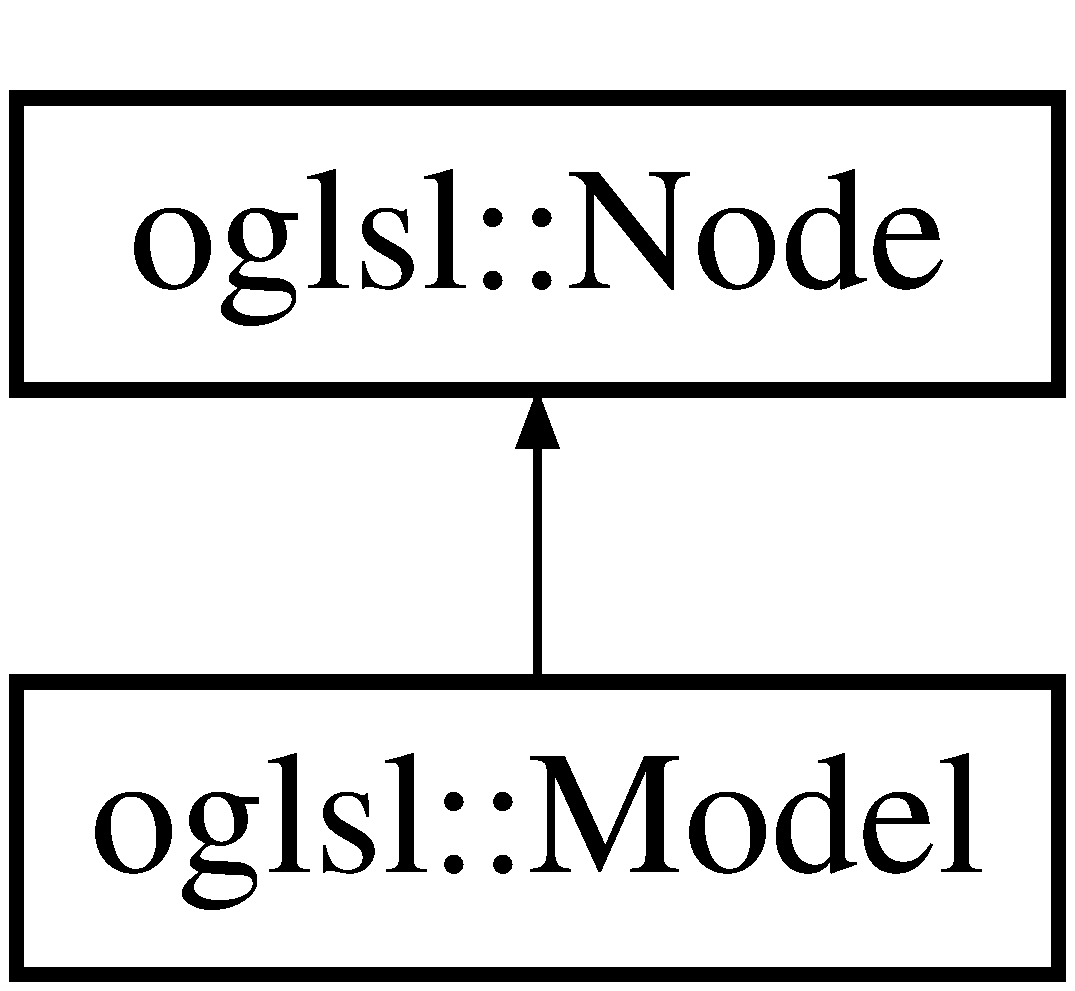
\includegraphics[height=2.000000cm]{classoglsl_1_1_model}
\end{center}
\end{figure}
\subsection*{Public Member Functions}
\begin{DoxyCompactItemize}
\item 
\mbox{\hyperlink{classoglsl_1_1_model_a1d1c934e59303cf5782cc3b45f80e462}{Model}} (char $\ast$path, shared\+\_\+ptr$<$ \mbox{\hyperlink{classoglsl_1_1_shader___program}{Shader\+\_\+\+Program}} $>$ shader)
\begin{DoxyCompactList}\small\item\em Initialices shader ids and loads model. \end{DoxyCompactList}\item 
\mbox{\hyperlink{classoglsl_1_1_model_ab3c8fe28157eaa2fd01646a0fc081f0f}{Model}} (char $\ast$path, shared\+\_\+ptr$<$ \mbox{\hyperlink{classoglsl_1_1_shader___program}{Shader\+\_\+\+Program}} $>$ shader, glm\+::vec3 color)
\begin{DoxyCompactList}\small\item\em Initialices shader ids, loads model and sets base color. \end{DoxyCompactList}\item 
void \mbox{\hyperlink{classoglsl_1_1_model_a22b769c49add4d10774e90466338c695}{render}} (const glm\+::mat4 \&parent\+\_\+model\+\_\+view) override
\begin{DoxyCompactList}\small\item\em Sets texture and uniforms, and render all meshes. \end{DoxyCompactList}\end{DoxyCompactItemize}
\subsection*{Additional Inherited Members}


\subsection{Detailed Description}
Represents a 3D model with several meshes. 

\subsection{Constructor \& Destructor Documentation}
\mbox{\Hypertarget{classoglsl_1_1_model_a1d1c934e59303cf5782cc3b45f80e462}\label{classoglsl_1_1_model_a1d1c934e59303cf5782cc3b45f80e462}} 
\index{oglsl\+::\+Model@{oglsl\+::\+Model}!Model@{Model}}
\index{Model@{Model}!oglsl\+::\+Model@{oglsl\+::\+Model}}
\subsubsection{\texorpdfstring{Model()}{Model()}\hspace{0.1cm}{\footnotesize\ttfamily [1/2]}}
{\footnotesize\ttfamily oglsl\+::\+Model\+::\+Model (\begin{DoxyParamCaption}\item[{char $\ast$}]{path,  }\item[{shared\+\_\+ptr$<$ \mbox{\hyperlink{classoglsl_1_1_shader___program}{Shader\+\_\+\+Program}} $>$}]{shader }\end{DoxyParamCaption})\hspace{0.3cm}{\ttfamily [inline]}}



Initialices shader ids and loads model. 

\mbox{\Hypertarget{classoglsl_1_1_model_ab3c8fe28157eaa2fd01646a0fc081f0f}\label{classoglsl_1_1_model_ab3c8fe28157eaa2fd01646a0fc081f0f}} 
\index{oglsl\+::\+Model@{oglsl\+::\+Model}!Model@{Model}}
\index{Model@{Model}!oglsl\+::\+Model@{oglsl\+::\+Model}}
\subsubsection{\texorpdfstring{Model()}{Model()}\hspace{0.1cm}{\footnotesize\ttfamily [2/2]}}
{\footnotesize\ttfamily oglsl\+::\+Model\+::\+Model (\begin{DoxyParamCaption}\item[{char $\ast$}]{path,  }\item[{shared\+\_\+ptr$<$ \mbox{\hyperlink{classoglsl_1_1_shader___program}{Shader\+\_\+\+Program}} $>$}]{shader,  }\item[{glm\+::vec3}]{color }\end{DoxyParamCaption})\hspace{0.3cm}{\ttfamily [inline]}}



Initialices shader ids, loads model and sets base color. 



\subsection{Member Function Documentation}
\mbox{\Hypertarget{classoglsl_1_1_model_a22b769c49add4d10774e90466338c695}\label{classoglsl_1_1_model_a22b769c49add4d10774e90466338c695}} 
\index{oglsl\+::\+Model@{oglsl\+::\+Model}!render@{render}}
\index{render@{render}!oglsl\+::\+Model@{oglsl\+::\+Model}}
\subsubsection{\texorpdfstring{render()}{render()}}
{\footnotesize\ttfamily void oglsl\+::\+Model\+::render (\begin{DoxyParamCaption}\item[{const glm\+::mat4 \&}]{parent\+\_\+model\+\_\+view }\end{DoxyParamCaption})\hspace{0.3cm}{\ttfamily [override]}, {\ttfamily [virtual]}}



Sets texture and uniforms, and render all meshes. 



Reimplemented from \mbox{\hyperlink{classoglsl_1_1_node_a09545b18a2d798327601a6251c091444}{oglsl\+::\+Node}}.



The documentation for this class was generated from the following files\+:\begin{DoxyCompactItemize}
\item 
D\+:/\+Git\+Kraken/3\+D\+Av\+\_\+2/src/\mbox{\hyperlink{_model_8hpp}{Model.\+hpp}}\item 
D\+:/\+Git\+Kraken/3\+D\+Av\+\_\+2/src/\mbox{\hyperlink{_model_8cpp}{Model.\+cpp}}\end{DoxyCompactItemize}

\hypertarget{classoglsl_1_1my_scene}{}\section{oglsl\+:\+:my\+Scene Class Reference}
\label{classoglsl_1_1my_scene}\index{oglsl\+::my\+Scene@{oglsl\+::my\+Scene}}


{\ttfamily \#include $<$my\+Scene.\+hpp$>$}

Inheritance diagram for oglsl\+:\+:my\+Scene\+:\begin{figure}[H]
\begin{center}
\leavevmode
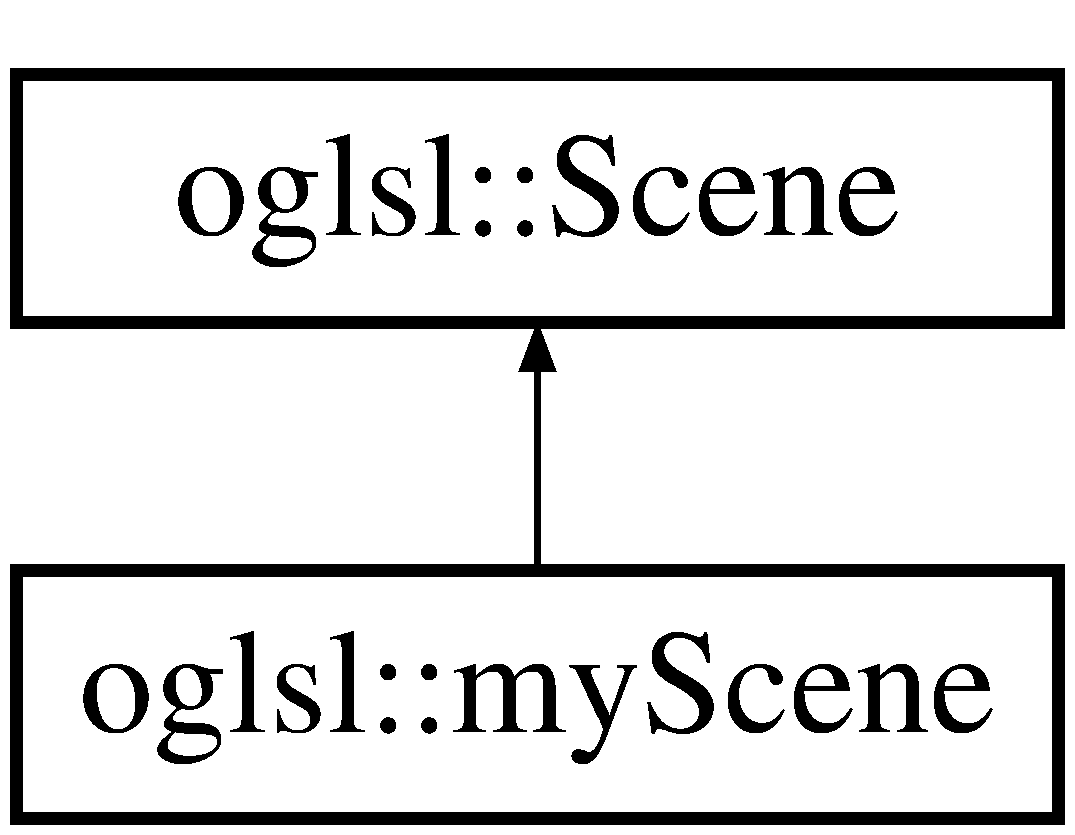
\includegraphics[height=2.000000cm]{classoglsl_1_1my_scene}
\end{center}
\end{figure}
\subsection*{Public Member Functions}
\begin{DoxyCompactItemize}
\item 
\mbox{\hyperlink{classoglsl_1_1my_scene_a1ea16fb5ced9ac6f5fea4db7688d6076}{my\+Scene}} ()
\item 
void \mbox{\hyperlink{classoglsl_1_1my_scene_aeab1e8cfe8c40f6110e1789a74008191}{process\+Input}} (\mbox{\hyperlink{classoglsl_1_1_input_a3b21d7328538e661f366af5d6059c197}{Input\+::\+Input\+Data}} input\+\_\+data) override
\begin{DoxyCompactList}\small\item\em Processes input data To implement in child scene. \end{DoxyCompactList}\item 
void \mbox{\hyperlink{classoglsl_1_1my_scene_a798dcfe11aee5c093013c59b665b6754}{update}} () override
\begin{DoxyCompactList}\small\item\em Updates the graph root. \end{DoxyCompactList}\end{DoxyCompactItemize}
\subsection*{Additional Inherited Members}


\subsection{Constructor \& Destructor Documentation}
\mbox{\Hypertarget{classoglsl_1_1my_scene_a1ea16fb5ced9ac6f5fea4db7688d6076}\label{classoglsl_1_1my_scene_a1ea16fb5ced9ac6f5fea4db7688d6076}} 
\index{oglsl\+::my\+Scene@{oglsl\+::my\+Scene}!my\+Scene@{my\+Scene}}
\index{my\+Scene@{my\+Scene}!oglsl\+::my\+Scene@{oglsl\+::my\+Scene}}
\subsubsection{\texorpdfstring{my\+Scene()}{myScene()}}
{\footnotesize\ttfamily oglsl\+::my\+Scene\+::my\+Scene (\begin{DoxyParamCaption}{ }\end{DoxyParamCaption})}



\subsection{Member Function Documentation}
\mbox{\Hypertarget{classoglsl_1_1my_scene_aeab1e8cfe8c40f6110e1789a74008191}\label{classoglsl_1_1my_scene_aeab1e8cfe8c40f6110e1789a74008191}} 
\index{oglsl\+::my\+Scene@{oglsl\+::my\+Scene}!process\+Input@{process\+Input}}
\index{process\+Input@{process\+Input}!oglsl\+::my\+Scene@{oglsl\+::my\+Scene}}
\subsubsection{\texorpdfstring{process\+Input()}{processInput()}}
{\footnotesize\ttfamily void oglsl\+::my\+Scene\+::process\+Input (\begin{DoxyParamCaption}\item[{\mbox{\hyperlink{classoglsl_1_1_input_a3b21d7328538e661f366af5d6059c197}{Input\+::\+Input\+Data}}}]{input\+\_\+data }\end{DoxyParamCaption})\hspace{0.3cm}{\ttfamily [override]}, {\ttfamily [virtual]}}



Processes input data To implement in child scene. 



Reimplemented from \mbox{\hyperlink{classoglsl_1_1_scene_a7884a3f2b7900aaf348a62ad23223c8e}{oglsl\+::\+Scene}}.

\mbox{\Hypertarget{classoglsl_1_1my_scene_a798dcfe11aee5c093013c59b665b6754}\label{classoglsl_1_1my_scene_a798dcfe11aee5c093013c59b665b6754}} 
\index{oglsl\+::my\+Scene@{oglsl\+::my\+Scene}!update@{update}}
\index{update@{update}!oglsl\+::my\+Scene@{oglsl\+::my\+Scene}}
\subsubsection{\texorpdfstring{update()}{update()}}
{\footnotesize\ttfamily void oglsl\+::my\+Scene\+::update (\begin{DoxyParamCaption}{ }\end{DoxyParamCaption})\hspace{0.3cm}{\ttfamily [override]}, {\ttfamily [virtual]}}



Updates the graph root. 



Reimplemented from \mbox{\hyperlink{classoglsl_1_1_scene_accbf0c6f23ccd909f63851c0bc547449}{oglsl\+::\+Scene}}.



The documentation for this class was generated from the following files\+:\begin{DoxyCompactItemize}
\item 
D\+:/\+Git\+Kraken/3\+D\+Av\+\_\+2/src/\mbox{\hyperlink{my_scene_8hpp}{my\+Scene.\+hpp}}\item 
D\+:/\+Git\+Kraken/3\+D\+Av\+\_\+2/src/\mbox{\hyperlink{my_scene_8cpp}{my\+Scene.\+cpp}}\end{DoxyCompactItemize}

\hypertarget{classoglsl_1_1_node}{}\section{oglsl\+:\+:Node Class Reference}
\label{classoglsl_1_1_node}\index{oglsl\+::\+Node@{oglsl\+::\+Node}}


Represents an object in the scene graph.  




{\ttfamily \#include $<$Node.\+hpp$>$}

Inheritance diagram for oglsl\+:\+:Node\+:\begin{figure}[H]
\begin{center}
\leavevmode
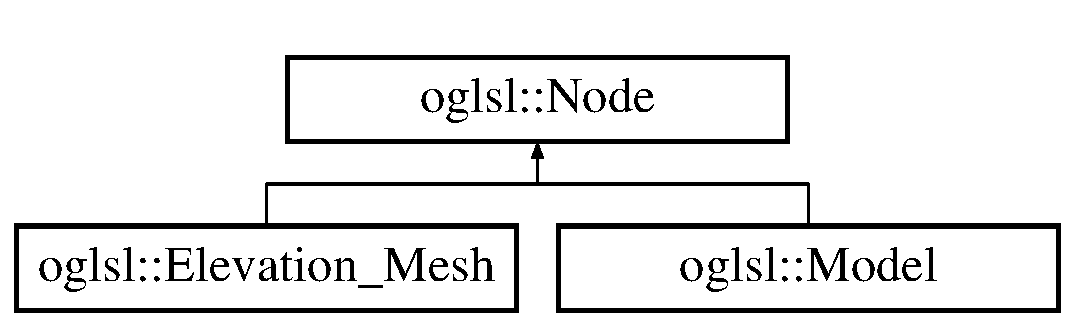
\includegraphics[height=2.000000cm]{classoglsl_1_1_node}
\end{center}
\end{figure}
\subsection*{Public Member Functions}
\begin{DoxyCompactItemize}
\item 
\mbox{\hyperlink{classoglsl_1_1_node_a485089d967532e58ecb6eaa1bcbb1185}{Node}} ()=default
\item 
virtual \mbox{\hyperlink{classoglsl_1_1_node_a45566d6c50af1f1676f0f11d3ef2b715}{$\sim$\+Node}} ()=default
\item 
virtual void \mbox{\hyperlink{classoglsl_1_1_node_a09545b18a2d798327601a6251c091444}{render}} (const glm\+::mat4 \&parent\+\_\+model\+\_\+view)
\begin{DoxyCompactList}\small\item\em Renders child nodes. \end{DoxyCompactList}\item 
virtual void \mbox{\hyperlink{classoglsl_1_1_node_af0c785449427102ed6922ea82e994577}{update}} ()
\begin{DoxyCompactList}\small\item\em Updates child nodes. \end{DoxyCompactList}\item 
void \mbox{\hyperlink{classoglsl_1_1_node_a2429fc76cc11f2b67a9161dc12517bab}{add\+Child}} (string name, shared\+\_\+ptr$<$ \mbox{\hyperlink{classoglsl_1_1_node}{Node}} $>$ child)
\begin{DoxyCompactList}\small\item\em Adds a new child to this node. \end{DoxyCompactList}\item 
map$<$ string, shared\+\_\+ptr$<$ \mbox{\hyperlink{classoglsl_1_1_node}{Node}} $>$ $>$ \mbox{\hyperlink{classoglsl_1_1_node_a7f3fb74d9bb97e2bc5f20ba75fbfa1e6}{get\+Children}} ()
\begin{DoxyCompactList}\small\item\em Returns a map with this node\textquotesingle{}s children. \end{DoxyCompactList}\item 
void \mbox{\hyperlink{classoglsl_1_1_node_a69b0ce077cfafe57a573a65299440949}{move}} (const glm\+::vec3 \&displacement)
\begin{DoxyCompactList}\small\item\em Displaces the current transform. \end{DoxyCompactList}\item 
void \mbox{\hyperlink{classoglsl_1_1_node_ab3463958740710e6af2a502ecd10d5ba}{rotate\+\_\+around\+\_\+x}} (float angle)
\begin{DoxyCompactList}\small\item\em Rotates transform around x axis. \end{DoxyCompactList}\item 
void \mbox{\hyperlink{classoglsl_1_1_node_a18862e40a37f13088bf454eb113e42d6}{rotate\+\_\+around\+\_\+y}} (float angle)
\begin{DoxyCompactList}\small\item\em Rotates transform around y axis. \end{DoxyCompactList}\item 
void \mbox{\hyperlink{classoglsl_1_1_node_afcd334ef611ba394879cd32be71d4c43}{rotate\+\_\+around\+\_\+z}} (float angle)
\begin{DoxyCompactList}\small\item\em Rotates transform around z axis. \end{DoxyCompactList}\item 
void \mbox{\hyperlink{classoglsl_1_1_node_a331a350e8311a310a77a109e6af6d135}{scale}} (float scale)
\begin{DoxyCompactList}\small\item\em Scales the transform in all axes. \end{DoxyCompactList}\end{DoxyCompactItemize}
\subsection*{Protected Attributes}
\begin{DoxyCompactItemize}
\item 
glm\+::mat4 \mbox{\hyperlink{classoglsl_1_1_node_a6b7251cdc6e62932d29f9094347b9e01}{transform}}
\end{DoxyCompactItemize}


\subsection{Detailed Description}
Represents an object in the scene graph. 

\subsection{Constructor \& Destructor Documentation}
\mbox{\Hypertarget{classoglsl_1_1_node_a485089d967532e58ecb6eaa1bcbb1185}\label{classoglsl_1_1_node_a485089d967532e58ecb6eaa1bcbb1185}} 
\index{oglsl\+::\+Node@{oglsl\+::\+Node}!Node@{Node}}
\index{Node@{Node}!oglsl\+::\+Node@{oglsl\+::\+Node}}
\subsubsection{\texorpdfstring{Node()}{Node()}}
{\footnotesize\ttfamily oglsl\+::\+Node\+::\+Node (\begin{DoxyParamCaption}{ }\end{DoxyParamCaption})\hspace{0.3cm}{\ttfamily [default]}}

\mbox{\Hypertarget{classoglsl_1_1_node_a45566d6c50af1f1676f0f11d3ef2b715}\label{classoglsl_1_1_node_a45566d6c50af1f1676f0f11d3ef2b715}} 
\index{oglsl\+::\+Node@{oglsl\+::\+Node}!````~Node@{$\sim$\+Node}}
\index{````~Node@{$\sim$\+Node}!oglsl\+::\+Node@{oglsl\+::\+Node}}
\subsubsection{\texorpdfstring{$\sim$\+Node()}{~Node()}}
{\footnotesize\ttfamily virtual oglsl\+::\+Node\+::$\sim$\+Node (\begin{DoxyParamCaption}{ }\end{DoxyParamCaption})\hspace{0.3cm}{\ttfamily [virtual]}, {\ttfamily [default]}}



\subsection{Member Function Documentation}
\mbox{\Hypertarget{classoglsl_1_1_node_a2429fc76cc11f2b67a9161dc12517bab}\label{classoglsl_1_1_node_a2429fc76cc11f2b67a9161dc12517bab}} 
\index{oglsl\+::\+Node@{oglsl\+::\+Node}!add\+Child@{add\+Child}}
\index{add\+Child@{add\+Child}!oglsl\+::\+Node@{oglsl\+::\+Node}}
\subsubsection{\texorpdfstring{add\+Child()}{addChild()}}
{\footnotesize\ttfamily void oglsl\+::\+Node\+::add\+Child (\begin{DoxyParamCaption}\item[{string}]{name,  }\item[{shared\+\_\+ptr$<$ \mbox{\hyperlink{classoglsl_1_1_node}{Node}} $>$}]{child }\end{DoxyParamCaption})\hspace{0.3cm}{\ttfamily [inline]}}



Adds a new child to this node. 

\mbox{\Hypertarget{classoglsl_1_1_node_a7f3fb74d9bb97e2bc5f20ba75fbfa1e6}\label{classoglsl_1_1_node_a7f3fb74d9bb97e2bc5f20ba75fbfa1e6}} 
\index{oglsl\+::\+Node@{oglsl\+::\+Node}!get\+Children@{get\+Children}}
\index{get\+Children@{get\+Children}!oglsl\+::\+Node@{oglsl\+::\+Node}}
\subsubsection{\texorpdfstring{get\+Children()}{getChildren()}}
{\footnotesize\ttfamily map$<$ string, shared\+\_\+ptr $<$ \mbox{\hyperlink{classoglsl_1_1_node}{Node}} $>$ $>$ oglsl\+::\+Node\+::get\+Children (\begin{DoxyParamCaption}{ }\end{DoxyParamCaption})\hspace{0.3cm}{\ttfamily [inline]}}



Returns a map with this node\textquotesingle{}s children. 

\mbox{\Hypertarget{classoglsl_1_1_node_a69b0ce077cfafe57a573a65299440949}\label{classoglsl_1_1_node_a69b0ce077cfafe57a573a65299440949}} 
\index{oglsl\+::\+Node@{oglsl\+::\+Node}!move@{move}}
\index{move@{move}!oglsl\+::\+Node@{oglsl\+::\+Node}}
\subsubsection{\texorpdfstring{move()}{move()}}
{\footnotesize\ttfamily void oglsl\+::\+Node\+::move (\begin{DoxyParamCaption}\item[{const glm\+::vec3 \&}]{displacement }\end{DoxyParamCaption})\hspace{0.3cm}{\ttfamily [inline]}}



Displaces the current transform. 

\mbox{\Hypertarget{classoglsl_1_1_node_a09545b18a2d798327601a6251c091444}\label{classoglsl_1_1_node_a09545b18a2d798327601a6251c091444}} 
\index{oglsl\+::\+Node@{oglsl\+::\+Node}!render@{render}}
\index{render@{render}!oglsl\+::\+Node@{oglsl\+::\+Node}}
\subsubsection{\texorpdfstring{render()}{render()}}
{\footnotesize\ttfamily virtual void oglsl\+::\+Node\+::render (\begin{DoxyParamCaption}\item[{const glm\+::mat4 \&}]{parent\+\_\+model\+\_\+view }\end{DoxyParamCaption})\hspace{0.3cm}{\ttfamily [inline]}, {\ttfamily [virtual]}}



Renders child nodes. 



Reimplemented in \mbox{\hyperlink{classoglsl_1_1_model_a22b769c49add4d10774e90466338c695}{oglsl\+::\+Model}}, and \mbox{\hyperlink{classoglsl_1_1_elevation___mesh_afb39dc1633680dccabb4b8da72ac4733}{oglsl\+::\+Elevation\+\_\+\+Mesh}}.

\mbox{\Hypertarget{classoglsl_1_1_node_ab3463958740710e6af2a502ecd10d5ba}\label{classoglsl_1_1_node_ab3463958740710e6af2a502ecd10d5ba}} 
\index{oglsl\+::\+Node@{oglsl\+::\+Node}!rotate\+\_\+around\+\_\+x@{rotate\+\_\+around\+\_\+x}}
\index{rotate\+\_\+around\+\_\+x@{rotate\+\_\+around\+\_\+x}!oglsl\+::\+Node@{oglsl\+::\+Node}}
\subsubsection{\texorpdfstring{rotate\+\_\+around\+\_\+x()}{rotate\_around\_x()}}
{\footnotesize\ttfamily void oglsl\+::\+Node\+::rotate\+\_\+around\+\_\+x (\begin{DoxyParamCaption}\item[{float}]{angle }\end{DoxyParamCaption})\hspace{0.3cm}{\ttfamily [inline]}}



Rotates transform around x axis. 

\mbox{\Hypertarget{classoglsl_1_1_node_a18862e40a37f13088bf454eb113e42d6}\label{classoglsl_1_1_node_a18862e40a37f13088bf454eb113e42d6}} 
\index{oglsl\+::\+Node@{oglsl\+::\+Node}!rotate\+\_\+around\+\_\+y@{rotate\+\_\+around\+\_\+y}}
\index{rotate\+\_\+around\+\_\+y@{rotate\+\_\+around\+\_\+y}!oglsl\+::\+Node@{oglsl\+::\+Node}}
\subsubsection{\texorpdfstring{rotate\+\_\+around\+\_\+y()}{rotate\_around\_y()}}
{\footnotesize\ttfamily void oglsl\+::\+Node\+::rotate\+\_\+around\+\_\+y (\begin{DoxyParamCaption}\item[{float}]{angle }\end{DoxyParamCaption})\hspace{0.3cm}{\ttfamily [inline]}}



Rotates transform around y axis. 

\mbox{\Hypertarget{classoglsl_1_1_node_afcd334ef611ba394879cd32be71d4c43}\label{classoglsl_1_1_node_afcd334ef611ba394879cd32be71d4c43}} 
\index{oglsl\+::\+Node@{oglsl\+::\+Node}!rotate\+\_\+around\+\_\+z@{rotate\+\_\+around\+\_\+z}}
\index{rotate\+\_\+around\+\_\+z@{rotate\+\_\+around\+\_\+z}!oglsl\+::\+Node@{oglsl\+::\+Node}}
\subsubsection{\texorpdfstring{rotate\+\_\+around\+\_\+z()}{rotate\_around\_z()}}
{\footnotesize\ttfamily void oglsl\+::\+Node\+::rotate\+\_\+around\+\_\+z (\begin{DoxyParamCaption}\item[{float}]{angle }\end{DoxyParamCaption})\hspace{0.3cm}{\ttfamily [inline]}}



Rotates transform around z axis. 

\mbox{\Hypertarget{classoglsl_1_1_node_a331a350e8311a310a77a109e6af6d135}\label{classoglsl_1_1_node_a331a350e8311a310a77a109e6af6d135}} 
\index{oglsl\+::\+Node@{oglsl\+::\+Node}!scale@{scale}}
\index{scale@{scale}!oglsl\+::\+Node@{oglsl\+::\+Node}}
\subsubsection{\texorpdfstring{scale()}{scale()}}
{\footnotesize\ttfamily void oglsl\+::\+Node\+::scale (\begin{DoxyParamCaption}\item[{float}]{scale }\end{DoxyParamCaption})\hspace{0.3cm}{\ttfamily [inline]}}



Scales the transform in all axes. 

\mbox{\Hypertarget{classoglsl_1_1_node_af0c785449427102ed6922ea82e994577}\label{classoglsl_1_1_node_af0c785449427102ed6922ea82e994577}} 
\index{oglsl\+::\+Node@{oglsl\+::\+Node}!update@{update}}
\index{update@{update}!oglsl\+::\+Node@{oglsl\+::\+Node}}
\subsubsection{\texorpdfstring{update()}{update()}}
{\footnotesize\ttfamily virtual void oglsl\+::\+Node\+::update (\begin{DoxyParamCaption}{ }\end{DoxyParamCaption})\hspace{0.3cm}{\ttfamily [inline]}, {\ttfamily [virtual]}}



Updates child nodes. 



\subsection{Member Data Documentation}
\mbox{\Hypertarget{classoglsl_1_1_node_a6b7251cdc6e62932d29f9094347b9e01}\label{classoglsl_1_1_node_a6b7251cdc6e62932d29f9094347b9e01}} 
\index{oglsl\+::\+Node@{oglsl\+::\+Node}!transform@{transform}}
\index{transform@{transform}!oglsl\+::\+Node@{oglsl\+::\+Node}}
\subsubsection{\texorpdfstring{transform}{transform}}
{\footnotesize\ttfamily glm\+::mat4 oglsl\+::\+Node\+::transform\hspace{0.3cm}{\ttfamily [protected]}}



The documentation for this class was generated from the following file\+:\begin{DoxyCompactItemize}
\item 
D\+:/\+Git\+Kraken/3\+D\+Av\+\_\+2/src/\mbox{\hyperlink{_node_8hpp}{Node.\+hpp}}\end{DoxyCompactItemize}

\hypertarget{classoglsl_1_1_scene}{}\section{oglsl\+:\+:Scene Class Reference}
\label{classoglsl_1_1_scene}\index{oglsl\+::\+Scene@{oglsl\+::\+Scene}}


Default scene setup.  




{\ttfamily \#include $<$Scene.\+hpp$>$}

Inheritance diagram for oglsl\+:\+:Scene\+:\begin{figure}[H]
\begin{center}
\leavevmode
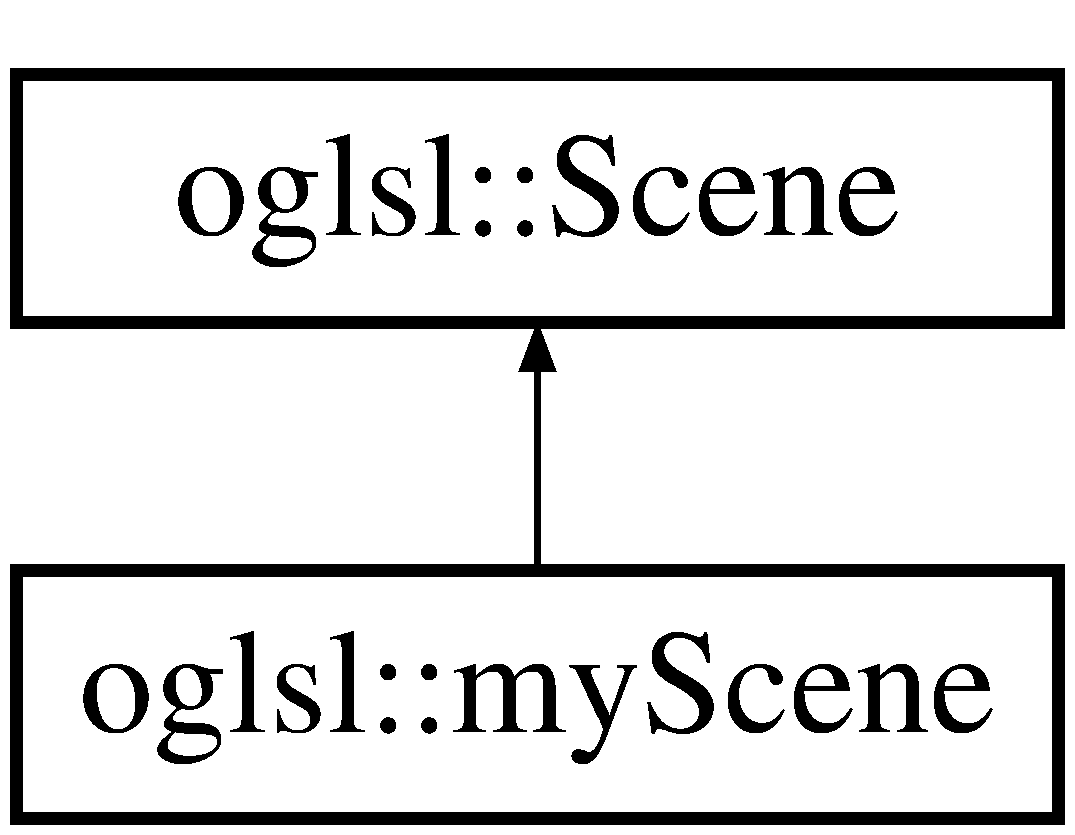
\includegraphics[height=2.000000cm]{classoglsl_1_1_scene}
\end{center}
\end{figure}
\subsection*{Public Member Functions}
\begin{DoxyCompactItemize}
\item 
\mbox{\hyperlink{classoglsl_1_1_scene_a1d13c881f3b0b7d4d7bd8d5225a50481}{Scene}} ()
\begin{DoxyCompactList}\small\item\em Sets up scene variables and default shaders. \end{DoxyCompactList}\item 
void \mbox{\hyperlink{classoglsl_1_1_scene_a1b1296aab1c81101473a38451c139819}{add}} (string name, shared\+\_\+ptr$<$ \mbox{\hyperlink{classoglsl_1_1_node}{Node}} $>$ node)
\begin{DoxyCompactList}\small\item\em Ads a new object to the scene. \end{DoxyCompactList}\item 
shared\+\_\+ptr$<$ \mbox{\hyperlink{classoglsl_1_1_node}{Node}} $>$ \mbox{\hyperlink{classoglsl_1_1_scene_a10b398b3e59b41c5fb0dbadb8120e0f3}{get\+Object}} (string name)
\begin{DoxyCompactList}\small\item\em Gets and object from the scene root. \end{DoxyCompactList}\item 
void \mbox{\hyperlink{classoglsl_1_1_scene_a94b552369f7653c854d38a1553c84288}{render}} ()
\begin{DoxyCompactList}\small\item\em Renders the scene. \end{DoxyCompactList}\item 
virtual void \mbox{\hyperlink{classoglsl_1_1_scene_accbf0c6f23ccd909f63851c0bc547449}{update}} ()
\begin{DoxyCompactList}\small\item\em Updates the graph root. \end{DoxyCompactList}\item 
void \mbox{\hyperlink{classoglsl_1_1_scene_a1eac687cef62ac021bfdd98749aa2ee5}{resize}} (int width, int height)
\begin{DoxyCompactList}\small\item\em Resizes the camera and projection\+\_\+matrix of all shaders. \end{DoxyCompactList}\item 
virtual void \mbox{\hyperlink{classoglsl_1_1_scene_a7884a3f2b7900aaf348a62ad23223c8e}{process\+Input}} (\mbox{\hyperlink{classoglsl_1_1_input_a3b21d7328538e661f366af5d6059c197}{Input\+::\+Input\+Data}} input\+\_\+data)
\begin{DoxyCompactList}\small\item\em Processes input data. \end{DoxyCompactList}\item 
virtual void \mbox{\hyperlink{classoglsl_1_1_scene_a91c975ee306374f17b9f348801f2ce3e}{configure\+\_\+light}} (shared\+\_\+ptr$<$ \mbox{\hyperlink{classoglsl_1_1_shader___program}{Shader\+\_\+\+Program}} $>$ program)
\begin{DoxyCompactList}\small\item\em Configures lights. \end{DoxyCompactList}\end{DoxyCompactItemize}
\subsection*{Protected Attributes}
\begin{DoxyCompactItemize}
\item 
\mbox{\hyperlink{classoglsl_1_1_camera}{Camera}} \mbox{\hyperlink{classoglsl_1_1_scene_a272ee5697b5bb4bfb725cb07b944dec4}{camera}}
\begin{DoxyCompactList}\small\item\em Main camera. \end{DoxyCompactList}\item 
shared\+\_\+ptr$<$ \mbox{\hyperlink{classoglsl_1_1_skybox}{Skybox}} $>$ \mbox{\hyperlink{classoglsl_1_1_scene_af01c494a85900703fc19e5bb7c757ebc}{skybox}}
\begin{DoxyCompactList}\small\item\em Default skybox. \end{DoxyCompactList}\item 
float \mbox{\hyperlink{classoglsl_1_1_scene_a3acba5c9ee3e2712b142550f5f06c488}{angle\+\_\+around\+\_\+x}}
\begin{DoxyCompactList}\small\item\em \mbox{\hyperlink{classoglsl_1_1_camera}{Camera}} angle around x axis. \end{DoxyCompactList}\item 
float \mbox{\hyperlink{classoglsl_1_1_scene_af8751fb0147fb71a1f4d5a0ddf94b99e}{angle\+\_\+around\+\_\+y}}
\begin{DoxyCompactList}\small\item\em \mbox{\hyperlink{classoglsl_1_1_camera}{Camera}} angle around y axis. \end{DoxyCompactList}\item 
map$<$ string, shared\+\_\+ptr$<$ \mbox{\hyperlink{classoglsl_1_1_shader___program}{Shader\+\_\+\+Program}} $>$ $>$ \mbox{\hyperlink{classoglsl_1_1_scene_ac60cfa73f999218a5c801308d29d33eb}{shaders}}
\begin{DoxyCompactList}\small\item\em Available shaders for the scene. \end{DoxyCompactList}\end{DoxyCompactItemize}


\subsection{Detailed Description}
Default scene setup. 

Can implement custom children scenes. 

\subsection{Constructor \& Destructor Documentation}
\mbox{\Hypertarget{classoglsl_1_1_scene_a1d13c881f3b0b7d4d7bd8d5225a50481}\label{classoglsl_1_1_scene_a1d13c881f3b0b7d4d7bd8d5225a50481}} 
\index{oglsl\+::\+Scene@{oglsl\+::\+Scene}!Scene@{Scene}}
\index{Scene@{Scene}!oglsl\+::\+Scene@{oglsl\+::\+Scene}}
\subsubsection{\texorpdfstring{Scene()}{Scene()}}
{\footnotesize\ttfamily oglsl\+::\+Scene\+::\+Scene (\begin{DoxyParamCaption}{ }\end{DoxyParamCaption})}



Sets up scene variables and default shaders. 



\subsection{Member Function Documentation}
\mbox{\Hypertarget{classoglsl_1_1_scene_a1b1296aab1c81101473a38451c139819}\label{classoglsl_1_1_scene_a1b1296aab1c81101473a38451c139819}} 
\index{oglsl\+::\+Scene@{oglsl\+::\+Scene}!add@{add}}
\index{add@{add}!oglsl\+::\+Scene@{oglsl\+::\+Scene}}
\subsubsection{\texorpdfstring{add()}{add()}}
{\footnotesize\ttfamily void oglsl\+::\+Scene\+::add (\begin{DoxyParamCaption}\item[{string}]{name,  }\item[{shared\+\_\+ptr$<$ \mbox{\hyperlink{classoglsl_1_1_node}{Node}} $>$}]{node }\end{DoxyParamCaption})\hspace{0.3cm}{\ttfamily [inline]}}



Ads a new object to the scene. 

\mbox{\Hypertarget{classoglsl_1_1_scene_a91c975ee306374f17b9f348801f2ce3e}\label{classoglsl_1_1_scene_a91c975ee306374f17b9f348801f2ce3e}} 
\index{oglsl\+::\+Scene@{oglsl\+::\+Scene}!configure\+\_\+light@{configure\+\_\+light}}
\index{configure\+\_\+light@{configure\+\_\+light}!oglsl\+::\+Scene@{oglsl\+::\+Scene}}
\subsubsection{\texorpdfstring{configure\+\_\+light()}{configure\_light()}}
{\footnotesize\ttfamily void oglsl\+::\+Scene\+::configure\+\_\+light (\begin{DoxyParamCaption}\item[{shared\+\_\+ptr$<$ \mbox{\hyperlink{classoglsl_1_1_shader___program}{Shader\+\_\+\+Program}} $>$}]{program }\end{DoxyParamCaption})\hspace{0.3cm}{\ttfamily [virtual]}}



Configures lights. 

Default setup. 
\begin{DoxyParams}{Parameters}
{\em program} & \mbox{\hyperlink{classoglsl_1_1_shader}{Shader}} to apply light parameters. Must support lightning. \\
\hline
\end{DoxyParams}
\mbox{\Hypertarget{classoglsl_1_1_scene_a10b398b3e59b41c5fb0dbadb8120e0f3}\label{classoglsl_1_1_scene_a10b398b3e59b41c5fb0dbadb8120e0f3}} 
\index{oglsl\+::\+Scene@{oglsl\+::\+Scene}!get\+Object@{get\+Object}}
\index{get\+Object@{get\+Object}!oglsl\+::\+Scene@{oglsl\+::\+Scene}}
\subsubsection{\texorpdfstring{get\+Object()}{getObject()}}
{\footnotesize\ttfamily shared\+\_\+ptr$<$ \mbox{\hyperlink{classoglsl_1_1_node}{Node}} $>$ oglsl\+::\+Scene\+::get\+Object (\begin{DoxyParamCaption}\item[{string}]{name }\end{DoxyParamCaption})\hspace{0.3cm}{\ttfamily [inline]}}



Gets and object from the scene root. 

\mbox{\Hypertarget{classoglsl_1_1_scene_a7884a3f2b7900aaf348a62ad23223c8e}\label{classoglsl_1_1_scene_a7884a3f2b7900aaf348a62ad23223c8e}} 
\index{oglsl\+::\+Scene@{oglsl\+::\+Scene}!process\+Input@{process\+Input}}
\index{process\+Input@{process\+Input}!oglsl\+::\+Scene@{oglsl\+::\+Scene}}
\subsubsection{\texorpdfstring{process\+Input()}{processInput()}}
{\footnotesize\ttfamily virtual void oglsl\+::\+Scene\+::process\+Input (\begin{DoxyParamCaption}\item[{\mbox{\hyperlink{classoglsl_1_1_input_a3b21d7328538e661f366af5d6059c197}{Input\+::\+Input\+Data}}}]{input\+\_\+data }\end{DoxyParamCaption})\hspace{0.3cm}{\ttfamily [inline]}, {\ttfamily [virtual]}}



Processes input data. 

To implement in child scene. 

Reimplemented in \mbox{\hyperlink{classoglsl_1_1my_scene_aeab1e8cfe8c40f6110e1789a74008191}{oglsl\+::my\+Scene}}.

\mbox{\Hypertarget{classoglsl_1_1_scene_a94b552369f7653c854d38a1553c84288}\label{classoglsl_1_1_scene_a94b552369f7653c854d38a1553c84288}} 
\index{oglsl\+::\+Scene@{oglsl\+::\+Scene}!render@{render}}
\index{render@{render}!oglsl\+::\+Scene@{oglsl\+::\+Scene}}
\subsubsection{\texorpdfstring{render()}{render()}}
{\footnotesize\ttfamily void oglsl\+::\+Scene\+::render (\begin{DoxyParamCaption}{ }\end{DoxyParamCaption})\hspace{0.3cm}{\ttfamily [inline]}}



Renders the scene. 

First renders the skybox and then all the objects in the graph. \mbox{\Hypertarget{classoglsl_1_1_scene_a1eac687cef62ac021bfdd98749aa2ee5}\label{classoglsl_1_1_scene_a1eac687cef62ac021bfdd98749aa2ee5}} 
\index{oglsl\+::\+Scene@{oglsl\+::\+Scene}!resize@{resize}}
\index{resize@{resize}!oglsl\+::\+Scene@{oglsl\+::\+Scene}}
\subsubsection{\texorpdfstring{resize()}{resize()}}
{\footnotesize\ttfamily void oglsl\+::\+Scene\+::resize (\begin{DoxyParamCaption}\item[{int}]{width,  }\item[{int}]{height }\end{DoxyParamCaption})\hspace{0.3cm}{\ttfamily [inline]}}



Resizes the camera and projection\+\_\+matrix of all shaders. 

\mbox{\Hypertarget{classoglsl_1_1_scene_accbf0c6f23ccd909f63851c0bc547449}\label{classoglsl_1_1_scene_accbf0c6f23ccd909f63851c0bc547449}} 
\index{oglsl\+::\+Scene@{oglsl\+::\+Scene}!update@{update}}
\index{update@{update}!oglsl\+::\+Scene@{oglsl\+::\+Scene}}
\subsubsection{\texorpdfstring{update()}{update()}}
{\footnotesize\ttfamily virtual void oglsl\+::\+Scene\+::update (\begin{DoxyParamCaption}{ }\end{DoxyParamCaption})\hspace{0.3cm}{\ttfamily [inline]}, {\ttfamily [virtual]}}



Updates the graph root. 



Reimplemented in \mbox{\hyperlink{classoglsl_1_1my_scene_a798dcfe11aee5c093013c59b665b6754}{oglsl\+::my\+Scene}}.



\subsection{Member Data Documentation}
\mbox{\Hypertarget{classoglsl_1_1_scene_a3acba5c9ee3e2712b142550f5f06c488}\label{classoglsl_1_1_scene_a3acba5c9ee3e2712b142550f5f06c488}} 
\index{oglsl\+::\+Scene@{oglsl\+::\+Scene}!angle\+\_\+around\+\_\+x@{angle\+\_\+around\+\_\+x}}
\index{angle\+\_\+around\+\_\+x@{angle\+\_\+around\+\_\+x}!oglsl\+::\+Scene@{oglsl\+::\+Scene}}
\subsubsection{\texorpdfstring{angle\+\_\+around\+\_\+x}{angle\_around\_x}}
{\footnotesize\ttfamily float oglsl\+::\+Scene\+::angle\+\_\+around\+\_\+x\hspace{0.3cm}{\ttfamily [protected]}}



\mbox{\hyperlink{classoglsl_1_1_camera}{Camera}} angle around x axis. 

\mbox{\Hypertarget{classoglsl_1_1_scene_af8751fb0147fb71a1f4d5a0ddf94b99e}\label{classoglsl_1_1_scene_af8751fb0147fb71a1f4d5a0ddf94b99e}} 
\index{oglsl\+::\+Scene@{oglsl\+::\+Scene}!angle\+\_\+around\+\_\+y@{angle\+\_\+around\+\_\+y}}
\index{angle\+\_\+around\+\_\+y@{angle\+\_\+around\+\_\+y}!oglsl\+::\+Scene@{oglsl\+::\+Scene}}
\subsubsection{\texorpdfstring{angle\+\_\+around\+\_\+y}{angle\_around\_y}}
{\footnotesize\ttfamily float oglsl\+::\+Scene\+::angle\+\_\+around\+\_\+y\hspace{0.3cm}{\ttfamily [protected]}}



\mbox{\hyperlink{classoglsl_1_1_camera}{Camera}} angle around y axis. 

\mbox{\Hypertarget{classoglsl_1_1_scene_a272ee5697b5bb4bfb725cb07b944dec4}\label{classoglsl_1_1_scene_a272ee5697b5bb4bfb725cb07b944dec4}} 
\index{oglsl\+::\+Scene@{oglsl\+::\+Scene}!camera@{camera}}
\index{camera@{camera}!oglsl\+::\+Scene@{oglsl\+::\+Scene}}
\subsubsection{\texorpdfstring{camera}{camera}}
{\footnotesize\ttfamily \mbox{\hyperlink{classoglsl_1_1_camera}{Camera}} oglsl\+::\+Scene\+::camera\hspace{0.3cm}{\ttfamily [protected]}}



Main camera. 

\mbox{\Hypertarget{classoglsl_1_1_scene_ac60cfa73f999218a5c801308d29d33eb}\label{classoglsl_1_1_scene_ac60cfa73f999218a5c801308d29d33eb}} 
\index{oglsl\+::\+Scene@{oglsl\+::\+Scene}!shaders@{shaders}}
\index{shaders@{shaders}!oglsl\+::\+Scene@{oglsl\+::\+Scene}}
\subsubsection{\texorpdfstring{shaders}{shaders}}
{\footnotesize\ttfamily map$<$ string, shared\+\_\+ptr$<$ \mbox{\hyperlink{classoglsl_1_1_shader___program}{Shader\+\_\+\+Program}} $>$ $>$ oglsl\+::\+Scene\+::shaders\hspace{0.3cm}{\ttfamily [protected]}}



Available shaders for the scene. 

\mbox{\Hypertarget{classoglsl_1_1_scene_af01c494a85900703fc19e5bb7c757ebc}\label{classoglsl_1_1_scene_af01c494a85900703fc19e5bb7c757ebc}} 
\index{oglsl\+::\+Scene@{oglsl\+::\+Scene}!skybox@{skybox}}
\index{skybox@{skybox}!oglsl\+::\+Scene@{oglsl\+::\+Scene}}
\subsubsection{\texorpdfstring{skybox}{skybox}}
{\footnotesize\ttfamily shared\+\_\+ptr$<$ \mbox{\hyperlink{classoglsl_1_1_skybox}{Skybox}} $>$ oglsl\+::\+Scene\+::skybox\hspace{0.3cm}{\ttfamily [protected]}}



Default skybox. 



The documentation for this class was generated from the following files\+:\begin{DoxyCompactItemize}
\item 
D\+:/\+Git\+Kraken/3\+D\+Av\+\_\+2/src/\mbox{\hyperlink{_scene_8hpp}{Scene.\+hpp}}\item 
D\+:/\+Git\+Kraken/3\+D\+Av\+\_\+2/src/\mbox{\hyperlink{_scene_8cpp}{Scene.\+cpp}}\end{DoxyCompactItemize}

\hypertarget{classoglsl_1_1_shader}{}\section{oglsl\+:\+:Shader Class Reference}
\label{classoglsl_1_1_shader}\index{oglsl\+::\+Shader@{oglsl\+::\+Shader}}


{\ttfamily \#include $<$Shader.\+hpp$>$}

Inheritance diagram for oglsl\+:\+:Shader\+:\begin{figure}[H]
\begin{center}
\leavevmode
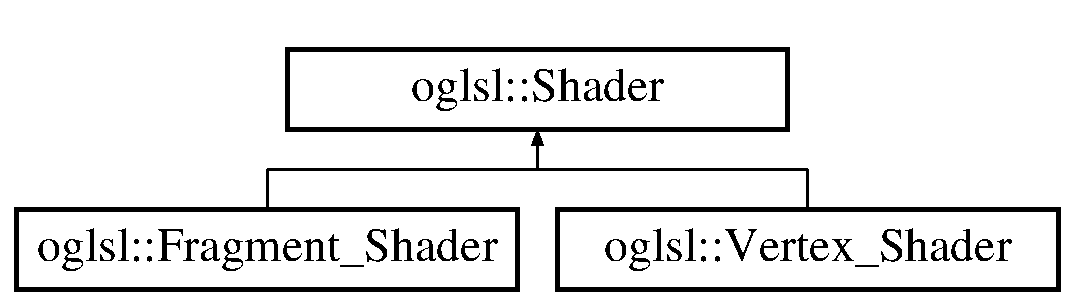
\includegraphics[height=2.000000cm]{classoglsl_1_1_shader}
\end{center}
\end{figure}
\subsection*{Classes}
\begin{DoxyCompactItemize}
\item 
class \mbox{\hyperlink{classoglsl_1_1_shader_1_1_source___code}{Source\+\_\+\+Code}}
\end{DoxyCompactItemize}
\subsection*{Public Member Functions}
\begin{DoxyCompactItemize}
\item 
bool \mbox{\hyperlink{classoglsl_1_1_shader_ade2f39e7d78cf5ac226fbe05b136b1c9}{is\+\_\+compiled}} () const
\item 
bool \mbox{\hyperlink{classoglsl_1_1_shader_a3de1ced039ae0d724d062263345d42ef}{compilation\+\_\+failed}} () const
\item 
const std\+::string \& \mbox{\hyperlink{classoglsl_1_1_shader_a5556801b4f5dffa82d3835003a73184a}{log}} () const
\item 
\mbox{\hyperlink{classoglsl_1_1_shader_af1bd8a3a30dff0e4f1c0e110db845169}{operator G\+Luint}} () const
\end{DoxyCompactItemize}
\subsection*{Protected Member Functions}
\begin{DoxyCompactItemize}
\item 
\mbox{\hyperlink{classoglsl_1_1_shader_a1560f72ace8a035eb367857156c0366f}{Shader}} (const \mbox{\hyperlink{classoglsl_1_1_shader_1_1_source___code}{Source\+\_\+\+Code}} \&source\+\_\+code, G\+Lenum shader\+\_\+type)
\item 
virtual \mbox{\hyperlink{classoglsl_1_1_shader_aea6c7b3bc4113abb6228dec6245b829a}{$\sim$\+Shader}} ()
\end{DoxyCompactItemize}


\subsection{Constructor \& Destructor Documentation}
\mbox{\Hypertarget{classoglsl_1_1_shader_a1560f72ace8a035eb367857156c0366f}\label{classoglsl_1_1_shader_a1560f72ace8a035eb367857156c0366f}} 
\index{oglsl\+::\+Shader@{oglsl\+::\+Shader}!Shader@{Shader}}
\index{Shader@{Shader}!oglsl\+::\+Shader@{oglsl\+::\+Shader}}
\subsubsection{\texorpdfstring{Shader()}{Shader()}}
{\footnotesize\ttfamily oglsl\+::\+Shader\+::\+Shader (\begin{DoxyParamCaption}\item[{const \mbox{\hyperlink{classoglsl_1_1_shader_1_1_source___code}{Source\+\_\+\+Code}} \&}]{source\+\_\+code,  }\item[{G\+Lenum}]{shader\+\_\+type }\end{DoxyParamCaption})\hspace{0.3cm}{\ttfamily [protected]}}

\mbox{\Hypertarget{classoglsl_1_1_shader_aea6c7b3bc4113abb6228dec6245b829a}\label{classoglsl_1_1_shader_aea6c7b3bc4113abb6228dec6245b829a}} 
\index{oglsl\+::\+Shader@{oglsl\+::\+Shader}!````~Shader@{$\sim$\+Shader}}
\index{````~Shader@{$\sim$\+Shader}!oglsl\+::\+Shader@{oglsl\+::\+Shader}}
\subsubsection{\texorpdfstring{$\sim$\+Shader()}{~Shader()}}
{\footnotesize\ttfamily oglsl\+::\+Shader\+::$\sim$\+Shader (\begin{DoxyParamCaption}{ }\end{DoxyParamCaption})\hspace{0.3cm}{\ttfamily [protected]}, {\ttfamily [virtual]}}



\subsection{Member Function Documentation}
\mbox{\Hypertarget{classoglsl_1_1_shader_a3de1ced039ae0d724d062263345d42ef}\label{classoglsl_1_1_shader_a3de1ced039ae0d724d062263345d42ef}} 
\index{oglsl\+::\+Shader@{oglsl\+::\+Shader}!compilation\+\_\+failed@{compilation\+\_\+failed}}
\index{compilation\+\_\+failed@{compilation\+\_\+failed}!oglsl\+::\+Shader@{oglsl\+::\+Shader}}
\subsubsection{\texorpdfstring{compilation\+\_\+failed()}{compilation\_failed()}}
{\footnotesize\ttfamily bool oglsl\+::\+Shader\+::compilation\+\_\+failed (\begin{DoxyParamCaption}{ }\end{DoxyParamCaption}) const\hspace{0.3cm}{\ttfamily [inline]}}

\mbox{\Hypertarget{classoglsl_1_1_shader_ade2f39e7d78cf5ac226fbe05b136b1c9}\label{classoglsl_1_1_shader_ade2f39e7d78cf5ac226fbe05b136b1c9}} 
\index{oglsl\+::\+Shader@{oglsl\+::\+Shader}!is\+\_\+compiled@{is\+\_\+compiled}}
\index{is\+\_\+compiled@{is\+\_\+compiled}!oglsl\+::\+Shader@{oglsl\+::\+Shader}}
\subsubsection{\texorpdfstring{is\+\_\+compiled()}{is\_compiled()}}
{\footnotesize\ttfamily bool oglsl\+::\+Shader\+::is\+\_\+compiled (\begin{DoxyParamCaption}{ }\end{DoxyParamCaption}) const\hspace{0.3cm}{\ttfamily [inline]}}

\mbox{\Hypertarget{classoglsl_1_1_shader_a5556801b4f5dffa82d3835003a73184a}\label{classoglsl_1_1_shader_a5556801b4f5dffa82d3835003a73184a}} 
\index{oglsl\+::\+Shader@{oglsl\+::\+Shader}!log@{log}}
\index{log@{log}!oglsl\+::\+Shader@{oglsl\+::\+Shader}}
\subsubsection{\texorpdfstring{log()}{log()}}
{\footnotesize\ttfamily const std\+::string\& oglsl\+::\+Shader\+::log (\begin{DoxyParamCaption}{ }\end{DoxyParamCaption}) const\hspace{0.3cm}{\ttfamily [inline]}}

\mbox{\Hypertarget{classoglsl_1_1_shader_af1bd8a3a30dff0e4f1c0e110db845169}\label{classoglsl_1_1_shader_af1bd8a3a30dff0e4f1c0e110db845169}} 
\index{oglsl\+::\+Shader@{oglsl\+::\+Shader}!operator G\+Luint@{operator G\+Luint}}
\index{operator G\+Luint@{operator G\+Luint}!oglsl\+::\+Shader@{oglsl\+::\+Shader}}
\subsubsection{\texorpdfstring{operator G\+Luint()}{operator GLuint()}}
{\footnotesize\ttfamily oglsl\+::\+Shader\+::operator G\+Luint (\begin{DoxyParamCaption}{ }\end{DoxyParamCaption}) const\hspace{0.3cm}{\ttfamily [inline]}}



The documentation for this class was generated from the following files\+:\begin{DoxyCompactItemize}
\item 
D\+:/\+Git\+Kraken/3\+D\+Av\+\_\+2/src/\mbox{\hyperlink{_shader_8hpp}{Shader.\+hpp}}\item 
D\+:/\+Git\+Kraken/3\+D\+Av\+\_\+2/src/\mbox{\hyperlink{_shader_8cpp}{Shader.\+cpp}}\end{DoxyCompactItemize}

\hypertarget{classoglsl_1_1_shader___program}{}\section{oglsl\+:\+:Shader\+\_\+\+Program Class Reference}
\label{classoglsl_1_1_shader___program}\index{oglsl\+::\+Shader\+\_\+\+Program@{oglsl\+::\+Shader\+\_\+\+Program}}


{\ttfamily \#include $<$Shader\+\_\+\+Program.\+hpp$>$}

\subsection*{Public Member Functions}
\begin{DoxyCompactItemize}
\item 
\mbox{\hyperlink{classoglsl_1_1_shader___program_ae5615f167ca4f6991ee4d7e75625e8e1}{Shader\+\_\+\+Program}} ()
\item 
\mbox{\hyperlink{classoglsl_1_1_shader___program_a632041a7db2cd19b7be88f4223085cdd}{$\sim$\+Shader\+\_\+\+Program}} ()
\item 
bool \mbox{\hyperlink{classoglsl_1_1_shader___program_abcf1f61c49728e6e4b2ed04bbdcc2413}{is\+\_\+usable}} () const
\item 
void \mbox{\hyperlink{classoglsl_1_1_shader___program_ac3dd7a7611533b0ad8a02dcca9a24a59}{attach}} (const \mbox{\hyperlink{classoglsl_1_1_shader}{Shader}} \&shader)
\item 
void \mbox{\hyperlink{classoglsl_1_1_shader___program_a54aec3bf30b58456f1f454e44618b724}{detach}} (const \mbox{\hyperlink{classoglsl_1_1_shader}{Shader}} \&shader)
\item 
bool \mbox{\hyperlink{classoglsl_1_1_shader___program_a91879ef2ebeee83ffddcbf6d7ec6904c}{link}} ()
\item 
void \mbox{\hyperlink{classoglsl_1_1_shader___program_ad68bd3ebd1b96464cb5708588e050044}{use}} () const
\item 
G\+Lint \mbox{\hyperlink{classoglsl_1_1_shader___program_a50588c2337e31efed044eb24f05d2e4e}{get\+\_\+uniform\+\_\+id}} (const char $\ast$identifier)
\item 
void \mbox{\hyperlink{classoglsl_1_1_shader___program_a28aae2ac780bb36b0753768bb65ecd2b}{set\+\_\+uniform\+\_\+value}} (G\+Lint uniform\+\_\+id, const G\+Lint \&value)
\item 
void \mbox{\hyperlink{classoglsl_1_1_shader___program_a04a17ba0d6065640fb54dd9a8671b2cb}{set\+\_\+uniform\+\_\+value}} (G\+Lint uniform\+\_\+id, const float \&value)
\item 
void \mbox{\hyperlink{classoglsl_1_1_shader___program_a86e83ef3d42661b55e7a14a08b1a568d}{set\+\_\+uniform\+\_\+value}} (G\+Lint uniform\+\_\+id, const Vector2f \&vector)
\item 
void \mbox{\hyperlink{classoglsl_1_1_shader___program_a9dd08db780ff6e96b31ea29609eb8a80}{set\+\_\+uniform\+\_\+value}} (G\+Lint uniform\+\_\+id, const Vector3f \&vector)
\item 
void \mbox{\hyperlink{classoglsl_1_1_shader___program_a557120833ebf82dd66f4b3ce120649b3}{set\+\_\+uniform\+\_\+value}} (G\+Lint uniform\+\_\+id, const Vector4f \&vector)
\item 
void \mbox{\hyperlink{classoglsl_1_1_shader___program_a664e80fef5a7c5941c79aff725fee938}{set\+\_\+uniform\+\_\+value}} (G\+Lint uniform\+\_\+id, const Matrix22f \&matrix)
\item 
void \mbox{\hyperlink{classoglsl_1_1_shader___program_a1504c5005186747a2311cf54ca1c1578}{set\+\_\+uniform\+\_\+value}} (G\+Lint uniform\+\_\+id, const Matrix33f \&matrix)
\item 
void \mbox{\hyperlink{classoglsl_1_1_shader___program_ad51c8c4a1556fa64b48f631d9cfd51c4}{set\+\_\+uniform\+\_\+value}} (G\+Lint uniform\+\_\+id, const Matrix44f \&matrix)
\item 
G\+Lint \mbox{\hyperlink{classoglsl_1_1_shader___program_a65d4cfa8e94ce9233bd65834b62df9e3}{get\+\_\+vertex\+\_\+attribute\+\_\+id}} (const char $\ast$identifier)
\item 
void \mbox{\hyperlink{classoglsl_1_1_shader___program_a31fd105d64825c2e7091ec536e7d15b3}{set\+\_\+vertex\+\_\+attribute}} (G\+Lint attribute\+\_\+id, const float \&value)
\item 
void \mbox{\hyperlink{classoglsl_1_1_shader___program_ab36f450b1a5d2ee375fb64ace2b89ccf}{set\+\_\+vertex\+\_\+attribute}} (G\+Lint attribute\+\_\+id, const Vector2f \&vector)
\item 
void \mbox{\hyperlink{classoglsl_1_1_shader___program_a95661ac1e32f6d3ffc1bfc81ce443e4a}{set\+\_\+vertex\+\_\+attribute}} (G\+Lint attribute\+\_\+id, const Vector3f \&vector)
\item 
void \mbox{\hyperlink{classoglsl_1_1_shader___program_a8e9053c1e6f9217ad9f12e245a0808a7}{set\+\_\+vertex\+\_\+attribute}} (G\+Lint attribute\+\_\+id, const Vector4f \&vector)
\item 
const std\+::string \& \mbox{\hyperlink{classoglsl_1_1_shader___program_addd674132d0eedf58f6bc92f0e446dc5}{log}} () const
\item 
\mbox{\hyperlink{classoglsl_1_1_shader___program_adad81ab380ceef8c885f084dfd6287c7}{operator G\+Luint}} () const
\end{DoxyCompactItemize}
\subsection*{Static Public Member Functions}
\begin{DoxyCompactItemize}
\item 
static void \mbox{\hyperlink{classoglsl_1_1_shader___program_a5513ced5c47dd2f020599ae4475bf907}{disable}} ()
\end{DoxyCompactItemize}


\subsection{Constructor \& Destructor Documentation}
\mbox{\Hypertarget{classoglsl_1_1_shader___program_ae5615f167ca4f6991ee4d7e75625e8e1}\label{classoglsl_1_1_shader___program_ae5615f167ca4f6991ee4d7e75625e8e1}} 
\index{oglsl\+::\+Shader\+\_\+\+Program@{oglsl\+::\+Shader\+\_\+\+Program}!Shader\+\_\+\+Program@{Shader\+\_\+\+Program}}
\index{Shader\+\_\+\+Program@{Shader\+\_\+\+Program}!oglsl\+::\+Shader\+\_\+\+Program@{oglsl\+::\+Shader\+\_\+\+Program}}
\subsubsection{\texorpdfstring{Shader\+\_\+\+Program()}{Shader\_Program()}}
{\footnotesize\ttfamily oglsl\+::\+Shader\+\_\+\+Program\+::\+Shader\+\_\+\+Program (\begin{DoxyParamCaption}{ }\end{DoxyParamCaption})\hspace{0.3cm}{\ttfamily [inline]}}

\mbox{\Hypertarget{classoglsl_1_1_shader___program_a632041a7db2cd19b7be88f4223085cdd}\label{classoglsl_1_1_shader___program_a632041a7db2cd19b7be88f4223085cdd}} 
\index{oglsl\+::\+Shader\+\_\+\+Program@{oglsl\+::\+Shader\+\_\+\+Program}!````~Shader\+\_\+\+Program@{$\sim$\+Shader\+\_\+\+Program}}
\index{````~Shader\+\_\+\+Program@{$\sim$\+Shader\+\_\+\+Program}!oglsl\+::\+Shader\+\_\+\+Program@{oglsl\+::\+Shader\+\_\+\+Program}}
\subsubsection{\texorpdfstring{$\sim$\+Shader\+\_\+\+Program()}{~Shader\_Program()}}
{\footnotesize\ttfamily oglsl\+::\+Shader\+\_\+\+Program\+::$\sim$\+Shader\+\_\+\+Program (\begin{DoxyParamCaption}{ }\end{DoxyParamCaption})\hspace{0.3cm}{\ttfamily [inline]}}



\subsection{Member Function Documentation}
\mbox{\Hypertarget{classoglsl_1_1_shader___program_ac3dd7a7611533b0ad8a02dcca9a24a59}\label{classoglsl_1_1_shader___program_ac3dd7a7611533b0ad8a02dcca9a24a59}} 
\index{oglsl\+::\+Shader\+\_\+\+Program@{oglsl\+::\+Shader\+\_\+\+Program}!attach@{attach}}
\index{attach@{attach}!oglsl\+::\+Shader\+\_\+\+Program@{oglsl\+::\+Shader\+\_\+\+Program}}
\subsubsection{\texorpdfstring{attach()}{attach()}}
{\footnotesize\ttfamily void oglsl\+::\+Shader\+\_\+\+Program\+::attach (\begin{DoxyParamCaption}\item[{const \mbox{\hyperlink{classoglsl_1_1_shader}{Shader}} \&}]{shader }\end{DoxyParamCaption})\hspace{0.3cm}{\ttfamily [inline]}}

\mbox{\Hypertarget{classoglsl_1_1_shader___program_a54aec3bf30b58456f1f454e44618b724}\label{classoglsl_1_1_shader___program_a54aec3bf30b58456f1f454e44618b724}} 
\index{oglsl\+::\+Shader\+\_\+\+Program@{oglsl\+::\+Shader\+\_\+\+Program}!detach@{detach}}
\index{detach@{detach}!oglsl\+::\+Shader\+\_\+\+Program@{oglsl\+::\+Shader\+\_\+\+Program}}
\subsubsection{\texorpdfstring{detach()}{detach()}}
{\footnotesize\ttfamily void oglsl\+::\+Shader\+\_\+\+Program\+::detach (\begin{DoxyParamCaption}\item[{const \mbox{\hyperlink{classoglsl_1_1_shader}{Shader}} \&}]{shader }\end{DoxyParamCaption})\hspace{0.3cm}{\ttfamily [inline]}}

\mbox{\Hypertarget{classoglsl_1_1_shader___program_a5513ced5c47dd2f020599ae4475bf907}\label{classoglsl_1_1_shader___program_a5513ced5c47dd2f020599ae4475bf907}} 
\index{oglsl\+::\+Shader\+\_\+\+Program@{oglsl\+::\+Shader\+\_\+\+Program}!disable@{disable}}
\index{disable@{disable}!oglsl\+::\+Shader\+\_\+\+Program@{oglsl\+::\+Shader\+\_\+\+Program}}
\subsubsection{\texorpdfstring{disable()}{disable()}}
{\footnotesize\ttfamily static void oglsl\+::\+Shader\+\_\+\+Program\+::disable (\begin{DoxyParamCaption}{ }\end{DoxyParamCaption})\hspace{0.3cm}{\ttfamily [inline]}, {\ttfamily [static]}}

\mbox{\Hypertarget{classoglsl_1_1_shader___program_a50588c2337e31efed044eb24f05d2e4e}\label{classoglsl_1_1_shader___program_a50588c2337e31efed044eb24f05d2e4e}} 
\index{oglsl\+::\+Shader\+\_\+\+Program@{oglsl\+::\+Shader\+\_\+\+Program}!get\+\_\+uniform\+\_\+id@{get\+\_\+uniform\+\_\+id}}
\index{get\+\_\+uniform\+\_\+id@{get\+\_\+uniform\+\_\+id}!oglsl\+::\+Shader\+\_\+\+Program@{oglsl\+::\+Shader\+\_\+\+Program}}
\subsubsection{\texorpdfstring{get\+\_\+uniform\+\_\+id()}{get\_uniform\_id()}}
{\footnotesize\ttfamily G\+Lint oglsl\+::\+Shader\+\_\+\+Program\+::get\+\_\+uniform\+\_\+id (\begin{DoxyParamCaption}\item[{const char $\ast$}]{identifier }\end{DoxyParamCaption})\hspace{0.3cm}{\ttfamily [inline]}}

\mbox{\Hypertarget{classoglsl_1_1_shader___program_a65d4cfa8e94ce9233bd65834b62df9e3}\label{classoglsl_1_1_shader___program_a65d4cfa8e94ce9233bd65834b62df9e3}} 
\index{oglsl\+::\+Shader\+\_\+\+Program@{oglsl\+::\+Shader\+\_\+\+Program}!get\+\_\+vertex\+\_\+attribute\+\_\+id@{get\+\_\+vertex\+\_\+attribute\+\_\+id}}
\index{get\+\_\+vertex\+\_\+attribute\+\_\+id@{get\+\_\+vertex\+\_\+attribute\+\_\+id}!oglsl\+::\+Shader\+\_\+\+Program@{oglsl\+::\+Shader\+\_\+\+Program}}
\subsubsection{\texorpdfstring{get\+\_\+vertex\+\_\+attribute\+\_\+id()}{get\_vertex\_attribute\_id()}}
{\footnotesize\ttfamily G\+Lint oglsl\+::\+Shader\+\_\+\+Program\+::get\+\_\+vertex\+\_\+attribute\+\_\+id (\begin{DoxyParamCaption}\item[{const char $\ast$}]{identifier }\end{DoxyParamCaption})\hspace{0.3cm}{\ttfamily [inline]}}

\mbox{\Hypertarget{classoglsl_1_1_shader___program_abcf1f61c49728e6e4b2ed04bbdcc2413}\label{classoglsl_1_1_shader___program_abcf1f61c49728e6e4b2ed04bbdcc2413}} 
\index{oglsl\+::\+Shader\+\_\+\+Program@{oglsl\+::\+Shader\+\_\+\+Program}!is\+\_\+usable@{is\+\_\+usable}}
\index{is\+\_\+usable@{is\+\_\+usable}!oglsl\+::\+Shader\+\_\+\+Program@{oglsl\+::\+Shader\+\_\+\+Program}}
\subsubsection{\texorpdfstring{is\+\_\+usable()}{is\_usable()}}
{\footnotesize\ttfamily bool oglsl\+::\+Shader\+\_\+\+Program\+::is\+\_\+usable (\begin{DoxyParamCaption}{ }\end{DoxyParamCaption}) const\hspace{0.3cm}{\ttfamily [inline]}}

\mbox{\Hypertarget{classoglsl_1_1_shader___program_a91879ef2ebeee83ffddcbf6d7ec6904c}\label{classoglsl_1_1_shader___program_a91879ef2ebeee83ffddcbf6d7ec6904c}} 
\index{oglsl\+::\+Shader\+\_\+\+Program@{oglsl\+::\+Shader\+\_\+\+Program}!link@{link}}
\index{link@{link}!oglsl\+::\+Shader\+\_\+\+Program@{oglsl\+::\+Shader\+\_\+\+Program}}
\subsubsection{\texorpdfstring{link()}{link()}}
{\footnotesize\ttfamily bool oglsl\+::\+Shader\+\_\+\+Program\+::link (\begin{DoxyParamCaption}{ }\end{DoxyParamCaption})}

\mbox{\Hypertarget{classoglsl_1_1_shader___program_addd674132d0eedf58f6bc92f0e446dc5}\label{classoglsl_1_1_shader___program_addd674132d0eedf58f6bc92f0e446dc5}} 
\index{oglsl\+::\+Shader\+\_\+\+Program@{oglsl\+::\+Shader\+\_\+\+Program}!log@{log}}
\index{log@{log}!oglsl\+::\+Shader\+\_\+\+Program@{oglsl\+::\+Shader\+\_\+\+Program}}
\subsubsection{\texorpdfstring{log()}{log()}}
{\footnotesize\ttfamily const std\+::string\& oglsl\+::\+Shader\+\_\+\+Program\+::log (\begin{DoxyParamCaption}{ }\end{DoxyParamCaption}) const\hspace{0.3cm}{\ttfamily [inline]}}

\mbox{\Hypertarget{classoglsl_1_1_shader___program_adad81ab380ceef8c885f084dfd6287c7}\label{classoglsl_1_1_shader___program_adad81ab380ceef8c885f084dfd6287c7}} 
\index{oglsl\+::\+Shader\+\_\+\+Program@{oglsl\+::\+Shader\+\_\+\+Program}!operator G\+Luint@{operator G\+Luint}}
\index{operator G\+Luint@{operator G\+Luint}!oglsl\+::\+Shader\+\_\+\+Program@{oglsl\+::\+Shader\+\_\+\+Program}}
\subsubsection{\texorpdfstring{operator G\+Luint()}{operator GLuint()}}
{\footnotesize\ttfamily oglsl\+::\+Shader\+\_\+\+Program\+::operator G\+Luint (\begin{DoxyParamCaption}{ }\end{DoxyParamCaption}) const\hspace{0.3cm}{\ttfamily [inline]}}

\mbox{\Hypertarget{classoglsl_1_1_shader___program_a28aae2ac780bb36b0753768bb65ecd2b}\label{classoglsl_1_1_shader___program_a28aae2ac780bb36b0753768bb65ecd2b}} 
\index{oglsl\+::\+Shader\+\_\+\+Program@{oglsl\+::\+Shader\+\_\+\+Program}!set\+\_\+uniform\+\_\+value@{set\+\_\+uniform\+\_\+value}}
\index{set\+\_\+uniform\+\_\+value@{set\+\_\+uniform\+\_\+value}!oglsl\+::\+Shader\+\_\+\+Program@{oglsl\+::\+Shader\+\_\+\+Program}}
\subsubsection{\texorpdfstring{set\+\_\+uniform\+\_\+value()}{set\_uniform\_value()}\hspace{0.1cm}{\footnotesize\ttfamily [1/8]}}
{\footnotesize\ttfamily void oglsl\+::\+Shader\+\_\+\+Program\+::set\+\_\+uniform\+\_\+value (\begin{DoxyParamCaption}\item[{G\+Lint}]{uniform\+\_\+id,  }\item[{const G\+Lint \&}]{value }\end{DoxyParamCaption})\hspace{0.3cm}{\ttfamily [inline]}}

\mbox{\Hypertarget{classoglsl_1_1_shader___program_a04a17ba0d6065640fb54dd9a8671b2cb}\label{classoglsl_1_1_shader___program_a04a17ba0d6065640fb54dd9a8671b2cb}} 
\index{oglsl\+::\+Shader\+\_\+\+Program@{oglsl\+::\+Shader\+\_\+\+Program}!set\+\_\+uniform\+\_\+value@{set\+\_\+uniform\+\_\+value}}
\index{set\+\_\+uniform\+\_\+value@{set\+\_\+uniform\+\_\+value}!oglsl\+::\+Shader\+\_\+\+Program@{oglsl\+::\+Shader\+\_\+\+Program}}
\subsubsection{\texorpdfstring{set\+\_\+uniform\+\_\+value()}{set\_uniform\_value()}\hspace{0.1cm}{\footnotesize\ttfamily [2/8]}}
{\footnotesize\ttfamily void oglsl\+::\+Shader\+\_\+\+Program\+::set\+\_\+uniform\+\_\+value (\begin{DoxyParamCaption}\item[{G\+Lint}]{uniform\+\_\+id,  }\item[{const float \&}]{value }\end{DoxyParamCaption})\hspace{0.3cm}{\ttfamily [inline]}}

\mbox{\Hypertarget{classoglsl_1_1_shader___program_a86e83ef3d42661b55e7a14a08b1a568d}\label{classoglsl_1_1_shader___program_a86e83ef3d42661b55e7a14a08b1a568d}} 
\index{oglsl\+::\+Shader\+\_\+\+Program@{oglsl\+::\+Shader\+\_\+\+Program}!set\+\_\+uniform\+\_\+value@{set\+\_\+uniform\+\_\+value}}
\index{set\+\_\+uniform\+\_\+value@{set\+\_\+uniform\+\_\+value}!oglsl\+::\+Shader\+\_\+\+Program@{oglsl\+::\+Shader\+\_\+\+Program}}
\subsubsection{\texorpdfstring{set\+\_\+uniform\+\_\+value()}{set\_uniform\_value()}\hspace{0.1cm}{\footnotesize\ttfamily [3/8]}}
{\footnotesize\ttfamily void oglsl\+::\+Shader\+\_\+\+Program\+::set\+\_\+uniform\+\_\+value (\begin{DoxyParamCaption}\item[{G\+Lint}]{uniform\+\_\+id,  }\item[{const Vector2f \&}]{vector }\end{DoxyParamCaption})\hspace{0.3cm}{\ttfamily [inline]}}

\mbox{\Hypertarget{classoglsl_1_1_shader___program_a9dd08db780ff6e96b31ea29609eb8a80}\label{classoglsl_1_1_shader___program_a9dd08db780ff6e96b31ea29609eb8a80}} 
\index{oglsl\+::\+Shader\+\_\+\+Program@{oglsl\+::\+Shader\+\_\+\+Program}!set\+\_\+uniform\+\_\+value@{set\+\_\+uniform\+\_\+value}}
\index{set\+\_\+uniform\+\_\+value@{set\+\_\+uniform\+\_\+value}!oglsl\+::\+Shader\+\_\+\+Program@{oglsl\+::\+Shader\+\_\+\+Program}}
\subsubsection{\texorpdfstring{set\+\_\+uniform\+\_\+value()}{set\_uniform\_value()}\hspace{0.1cm}{\footnotesize\ttfamily [4/8]}}
{\footnotesize\ttfamily void oglsl\+::\+Shader\+\_\+\+Program\+::set\+\_\+uniform\+\_\+value (\begin{DoxyParamCaption}\item[{G\+Lint}]{uniform\+\_\+id,  }\item[{const Vector3f \&}]{vector }\end{DoxyParamCaption})\hspace{0.3cm}{\ttfamily [inline]}}

\mbox{\Hypertarget{classoglsl_1_1_shader___program_a557120833ebf82dd66f4b3ce120649b3}\label{classoglsl_1_1_shader___program_a557120833ebf82dd66f4b3ce120649b3}} 
\index{oglsl\+::\+Shader\+\_\+\+Program@{oglsl\+::\+Shader\+\_\+\+Program}!set\+\_\+uniform\+\_\+value@{set\+\_\+uniform\+\_\+value}}
\index{set\+\_\+uniform\+\_\+value@{set\+\_\+uniform\+\_\+value}!oglsl\+::\+Shader\+\_\+\+Program@{oglsl\+::\+Shader\+\_\+\+Program}}
\subsubsection{\texorpdfstring{set\+\_\+uniform\+\_\+value()}{set\_uniform\_value()}\hspace{0.1cm}{\footnotesize\ttfamily [5/8]}}
{\footnotesize\ttfamily void oglsl\+::\+Shader\+\_\+\+Program\+::set\+\_\+uniform\+\_\+value (\begin{DoxyParamCaption}\item[{G\+Lint}]{uniform\+\_\+id,  }\item[{const Vector4f \&}]{vector }\end{DoxyParamCaption})\hspace{0.3cm}{\ttfamily [inline]}}

\mbox{\Hypertarget{classoglsl_1_1_shader___program_a664e80fef5a7c5941c79aff725fee938}\label{classoglsl_1_1_shader___program_a664e80fef5a7c5941c79aff725fee938}} 
\index{oglsl\+::\+Shader\+\_\+\+Program@{oglsl\+::\+Shader\+\_\+\+Program}!set\+\_\+uniform\+\_\+value@{set\+\_\+uniform\+\_\+value}}
\index{set\+\_\+uniform\+\_\+value@{set\+\_\+uniform\+\_\+value}!oglsl\+::\+Shader\+\_\+\+Program@{oglsl\+::\+Shader\+\_\+\+Program}}
\subsubsection{\texorpdfstring{set\+\_\+uniform\+\_\+value()}{set\_uniform\_value()}\hspace{0.1cm}{\footnotesize\ttfamily [6/8]}}
{\footnotesize\ttfamily void oglsl\+::\+Shader\+\_\+\+Program\+::set\+\_\+uniform\+\_\+value (\begin{DoxyParamCaption}\item[{G\+Lint}]{uniform\+\_\+id,  }\item[{const Matrix22f \&}]{matrix }\end{DoxyParamCaption})\hspace{0.3cm}{\ttfamily [inline]}}

\mbox{\Hypertarget{classoglsl_1_1_shader___program_a1504c5005186747a2311cf54ca1c1578}\label{classoglsl_1_1_shader___program_a1504c5005186747a2311cf54ca1c1578}} 
\index{oglsl\+::\+Shader\+\_\+\+Program@{oglsl\+::\+Shader\+\_\+\+Program}!set\+\_\+uniform\+\_\+value@{set\+\_\+uniform\+\_\+value}}
\index{set\+\_\+uniform\+\_\+value@{set\+\_\+uniform\+\_\+value}!oglsl\+::\+Shader\+\_\+\+Program@{oglsl\+::\+Shader\+\_\+\+Program}}
\subsubsection{\texorpdfstring{set\+\_\+uniform\+\_\+value()}{set\_uniform\_value()}\hspace{0.1cm}{\footnotesize\ttfamily [7/8]}}
{\footnotesize\ttfamily void oglsl\+::\+Shader\+\_\+\+Program\+::set\+\_\+uniform\+\_\+value (\begin{DoxyParamCaption}\item[{G\+Lint}]{uniform\+\_\+id,  }\item[{const Matrix33f \&}]{matrix }\end{DoxyParamCaption})\hspace{0.3cm}{\ttfamily [inline]}}

\mbox{\Hypertarget{classoglsl_1_1_shader___program_ad51c8c4a1556fa64b48f631d9cfd51c4}\label{classoglsl_1_1_shader___program_ad51c8c4a1556fa64b48f631d9cfd51c4}} 
\index{oglsl\+::\+Shader\+\_\+\+Program@{oglsl\+::\+Shader\+\_\+\+Program}!set\+\_\+uniform\+\_\+value@{set\+\_\+uniform\+\_\+value}}
\index{set\+\_\+uniform\+\_\+value@{set\+\_\+uniform\+\_\+value}!oglsl\+::\+Shader\+\_\+\+Program@{oglsl\+::\+Shader\+\_\+\+Program}}
\subsubsection{\texorpdfstring{set\+\_\+uniform\+\_\+value()}{set\_uniform\_value()}\hspace{0.1cm}{\footnotesize\ttfamily [8/8]}}
{\footnotesize\ttfamily void oglsl\+::\+Shader\+\_\+\+Program\+::set\+\_\+uniform\+\_\+value (\begin{DoxyParamCaption}\item[{G\+Lint}]{uniform\+\_\+id,  }\item[{const Matrix44f \&}]{matrix }\end{DoxyParamCaption})\hspace{0.3cm}{\ttfamily [inline]}}

\mbox{\Hypertarget{classoglsl_1_1_shader___program_a31fd105d64825c2e7091ec536e7d15b3}\label{classoglsl_1_1_shader___program_a31fd105d64825c2e7091ec536e7d15b3}} 
\index{oglsl\+::\+Shader\+\_\+\+Program@{oglsl\+::\+Shader\+\_\+\+Program}!set\+\_\+vertex\+\_\+attribute@{set\+\_\+vertex\+\_\+attribute}}
\index{set\+\_\+vertex\+\_\+attribute@{set\+\_\+vertex\+\_\+attribute}!oglsl\+::\+Shader\+\_\+\+Program@{oglsl\+::\+Shader\+\_\+\+Program}}
\subsubsection{\texorpdfstring{set\+\_\+vertex\+\_\+attribute()}{set\_vertex\_attribute()}\hspace{0.1cm}{\footnotesize\ttfamily [1/4]}}
{\footnotesize\ttfamily void oglsl\+::\+Shader\+\_\+\+Program\+::set\+\_\+vertex\+\_\+attribute (\begin{DoxyParamCaption}\item[{G\+Lint}]{attribute\+\_\+id,  }\item[{const float \&}]{value }\end{DoxyParamCaption})\hspace{0.3cm}{\ttfamily [inline]}}

\mbox{\Hypertarget{classoglsl_1_1_shader___program_ab36f450b1a5d2ee375fb64ace2b89ccf}\label{classoglsl_1_1_shader___program_ab36f450b1a5d2ee375fb64ace2b89ccf}} 
\index{oglsl\+::\+Shader\+\_\+\+Program@{oglsl\+::\+Shader\+\_\+\+Program}!set\+\_\+vertex\+\_\+attribute@{set\+\_\+vertex\+\_\+attribute}}
\index{set\+\_\+vertex\+\_\+attribute@{set\+\_\+vertex\+\_\+attribute}!oglsl\+::\+Shader\+\_\+\+Program@{oglsl\+::\+Shader\+\_\+\+Program}}
\subsubsection{\texorpdfstring{set\+\_\+vertex\+\_\+attribute()}{set\_vertex\_attribute()}\hspace{0.1cm}{\footnotesize\ttfamily [2/4]}}
{\footnotesize\ttfamily void oglsl\+::\+Shader\+\_\+\+Program\+::set\+\_\+vertex\+\_\+attribute (\begin{DoxyParamCaption}\item[{G\+Lint}]{attribute\+\_\+id,  }\item[{const Vector2f \&}]{vector }\end{DoxyParamCaption})\hspace{0.3cm}{\ttfamily [inline]}}

\mbox{\Hypertarget{classoglsl_1_1_shader___program_a95661ac1e32f6d3ffc1bfc81ce443e4a}\label{classoglsl_1_1_shader___program_a95661ac1e32f6d3ffc1bfc81ce443e4a}} 
\index{oglsl\+::\+Shader\+\_\+\+Program@{oglsl\+::\+Shader\+\_\+\+Program}!set\+\_\+vertex\+\_\+attribute@{set\+\_\+vertex\+\_\+attribute}}
\index{set\+\_\+vertex\+\_\+attribute@{set\+\_\+vertex\+\_\+attribute}!oglsl\+::\+Shader\+\_\+\+Program@{oglsl\+::\+Shader\+\_\+\+Program}}
\subsubsection{\texorpdfstring{set\+\_\+vertex\+\_\+attribute()}{set\_vertex\_attribute()}\hspace{0.1cm}{\footnotesize\ttfamily [3/4]}}
{\footnotesize\ttfamily void oglsl\+::\+Shader\+\_\+\+Program\+::set\+\_\+vertex\+\_\+attribute (\begin{DoxyParamCaption}\item[{G\+Lint}]{attribute\+\_\+id,  }\item[{const Vector3f \&}]{vector }\end{DoxyParamCaption})\hspace{0.3cm}{\ttfamily [inline]}}

\mbox{\Hypertarget{classoglsl_1_1_shader___program_a8e9053c1e6f9217ad9f12e245a0808a7}\label{classoglsl_1_1_shader___program_a8e9053c1e6f9217ad9f12e245a0808a7}} 
\index{oglsl\+::\+Shader\+\_\+\+Program@{oglsl\+::\+Shader\+\_\+\+Program}!set\+\_\+vertex\+\_\+attribute@{set\+\_\+vertex\+\_\+attribute}}
\index{set\+\_\+vertex\+\_\+attribute@{set\+\_\+vertex\+\_\+attribute}!oglsl\+::\+Shader\+\_\+\+Program@{oglsl\+::\+Shader\+\_\+\+Program}}
\subsubsection{\texorpdfstring{set\+\_\+vertex\+\_\+attribute()}{set\_vertex\_attribute()}\hspace{0.1cm}{\footnotesize\ttfamily [4/4]}}
{\footnotesize\ttfamily void oglsl\+::\+Shader\+\_\+\+Program\+::set\+\_\+vertex\+\_\+attribute (\begin{DoxyParamCaption}\item[{G\+Lint}]{attribute\+\_\+id,  }\item[{const Vector4f \&}]{vector }\end{DoxyParamCaption})\hspace{0.3cm}{\ttfamily [inline]}}

\mbox{\Hypertarget{classoglsl_1_1_shader___program_ad68bd3ebd1b96464cb5708588e050044}\label{classoglsl_1_1_shader___program_ad68bd3ebd1b96464cb5708588e050044}} 
\index{oglsl\+::\+Shader\+\_\+\+Program@{oglsl\+::\+Shader\+\_\+\+Program}!use@{use}}
\index{use@{use}!oglsl\+::\+Shader\+\_\+\+Program@{oglsl\+::\+Shader\+\_\+\+Program}}
\subsubsection{\texorpdfstring{use()}{use()}}
{\footnotesize\ttfamily void oglsl\+::\+Shader\+\_\+\+Program\+::use (\begin{DoxyParamCaption}{ }\end{DoxyParamCaption}) const\hspace{0.3cm}{\ttfamily [inline]}}



The documentation for this class was generated from the following files\+:\begin{DoxyCompactItemize}
\item 
D\+:/\+Git\+Kraken/3\+D\+Av\+\_\+2/src/\mbox{\hyperlink{_shader___program_8hpp}{Shader\+\_\+\+Program.\+hpp}}\item 
D\+:/\+Git\+Kraken/3\+D\+Av\+\_\+2/src/\mbox{\hyperlink{_shader___program_8cpp}{Shader\+\_\+\+Program.\+cpp}}\end{DoxyCompactItemize}

\hypertarget{classoglsl_1_1_skybox}{}\section{oglsl\+:\+:Skybox Class Reference}
\label{classoglsl_1_1_skybox}\index{oglsl\+::\+Skybox@{oglsl\+::\+Skybox}}


Represents the cubemap texture rendered as the scene background.  




{\ttfamily \#include $<$Skybox.\+hpp$>$}

\subsection*{Public Member Functions}
\begin{DoxyCompactItemize}
\item 
\mbox{\hyperlink{classoglsl_1_1_skybox_a1fd7b807be900efc97e0e1ab2f0e0d1b}{Skybox}} (const std\+::string \&texture\+\_\+path, std\+::shared\+\_\+ptr$<$ \mbox{\hyperlink{classoglsl_1_1_shader___program}{Shader\+\_\+\+Program}} $>$ shader)
\begin{DoxyCompactList}\small\item\em Creates the cube ans inits the skybox shader. \end{DoxyCompactList}\item 
\mbox{\hyperlink{classoglsl_1_1_skybox_ae49b37d4211f0f6f3fb7de0199324a3f}{$\sim$\+Skybox}} ()
\item 
void \mbox{\hyperlink{classoglsl_1_1_skybox_a2ee558805867f1acdfab64f689c41f76}{render}} (const \mbox{\hyperlink{classoglsl_1_1_camera}{Camera}} \&camera)
\begin{DoxyCompactList}\small\item\em Renders the skybox. \end{DoxyCompactList}\end{DoxyCompactItemize}


\subsection{Detailed Description}
Represents the cubemap texture rendered as the scene background. 

\subsection{Constructor \& Destructor Documentation}
\mbox{\Hypertarget{classoglsl_1_1_skybox_a1fd7b807be900efc97e0e1ab2f0e0d1b}\label{classoglsl_1_1_skybox_a1fd7b807be900efc97e0e1ab2f0e0d1b}} 
\index{oglsl\+::\+Skybox@{oglsl\+::\+Skybox}!Skybox@{Skybox}}
\index{Skybox@{Skybox}!oglsl\+::\+Skybox@{oglsl\+::\+Skybox}}
\subsubsection{\texorpdfstring{Skybox()}{Skybox()}}
{\footnotesize\ttfamily oglsl\+::\+Skybox\+::\+Skybox (\begin{DoxyParamCaption}\item[{const std\+::string \&}]{texture\+\_\+path,  }\item[{std\+::shared\+\_\+ptr$<$ \mbox{\hyperlink{classoglsl_1_1_shader___program}{Shader\+\_\+\+Program}} $>$}]{shader }\end{DoxyParamCaption})}



Creates the cube ans inits the skybox shader. 

\mbox{\Hypertarget{classoglsl_1_1_skybox_ae49b37d4211f0f6f3fb7de0199324a3f}\label{classoglsl_1_1_skybox_ae49b37d4211f0f6f3fb7de0199324a3f}} 
\index{oglsl\+::\+Skybox@{oglsl\+::\+Skybox}!````~Skybox@{$\sim$\+Skybox}}
\index{````~Skybox@{$\sim$\+Skybox}!oglsl\+::\+Skybox@{oglsl\+::\+Skybox}}
\subsubsection{\texorpdfstring{$\sim$\+Skybox()}{~Skybox()}}
{\footnotesize\ttfamily oglsl\+::\+Skybox\+::$\sim$\+Skybox (\begin{DoxyParamCaption}{ }\end{DoxyParamCaption})}



\subsection{Member Function Documentation}
\mbox{\Hypertarget{classoglsl_1_1_skybox_a2ee558805867f1acdfab64f689c41f76}\label{classoglsl_1_1_skybox_a2ee558805867f1acdfab64f689c41f76}} 
\index{oglsl\+::\+Skybox@{oglsl\+::\+Skybox}!render@{render}}
\index{render@{render}!oglsl\+::\+Skybox@{oglsl\+::\+Skybox}}
\subsubsection{\texorpdfstring{render()}{render()}}
{\footnotesize\ttfamily void oglsl\+::\+Skybox\+::render (\begin{DoxyParamCaption}\item[{const \mbox{\hyperlink{classoglsl_1_1_camera}{Camera}} \&}]{camera }\end{DoxyParamCaption})}



Renders the skybox. 

Be careful when setting the camera near pane, as the skybox cube is 1x1x1. 0.\+5 is a safe value. 
\begin{DoxyParams}{Parameters}
{\em camera} & \mbox{\hyperlink{classoglsl_1_1_scene}{Scene}} camera. \\
\hline
\end{DoxyParams}


The documentation for this class was generated from the following files\+:\begin{DoxyCompactItemize}
\item 
D\+:/\+Git\+Kraken/3\+D\+Av\+\_\+2/src/\mbox{\hyperlink{_skybox_8hpp}{Skybox.\+hpp}}\item 
D\+:/\+Git\+Kraken/3\+D\+Av\+\_\+2/src/\mbox{\hyperlink{_skybox_8cpp}{Skybox.\+cpp}}\end{DoxyCompactItemize}

\hypertarget{classoglsl_1_1_shader_1_1_source___code}{}\section{oglsl\+:\+:Shader\+:\+:Source\+\_\+\+Code Class Reference}
\label{classoglsl_1_1_shader_1_1_source___code}\index{oglsl\+::\+Shader\+::\+Source\+\_\+\+Code@{oglsl\+::\+Shader\+::\+Source\+\_\+\+Code}}


{\ttfamily \#include $<$Shader.\+hpp$>$}

\subsection*{Public Member Functions}
\begin{DoxyCompactItemize}
\item 
size\+\_\+t \mbox{\hyperlink{classoglsl_1_1_shader_1_1_source___code_ab1ea89bfdad1d955982b2821457f9d13}{size}} () const
\item 
bool \mbox{\hyperlink{classoglsl_1_1_shader_1_1_source___code_a3da37bbe585ebd1e5d3c22e5fbdbf73d}{is\+\_\+empty}} () const
\item 
bool \mbox{\hyperlink{classoglsl_1_1_shader_1_1_source___code_ad67238c4cf313b838a94e7f4a41a0eb6}{is\+\_\+not\+\_\+empty}} () const
\item 
\mbox{\hyperlink{classoglsl_1_1_shader_1_1_source___code_a1305244d85aabc655fba7cf4f55cc5b4}{operator const std\+::string \&}} () const
\item 
\mbox{\hyperlink{classoglsl_1_1_shader_1_1_source___code_a0e0ee6581e24a6633294a6db926b8b7c}{operator const char $\ast$}} () const
\end{DoxyCompactItemize}
\subsection*{Static Public Member Functions}
\begin{DoxyCompactItemize}
\item 
static \mbox{\hyperlink{classoglsl_1_1_shader_1_1_source___code}{Source\+\_\+\+Code}} \mbox{\hyperlink{classoglsl_1_1_shader_1_1_source___code_a9bb3f9ec92c2ca8e88ed4505ee3673d5}{from\+\_\+string}} (const std\+::string \&source\+\_\+code\+\_\+string)
\item 
static \mbox{\hyperlink{classoglsl_1_1_shader_1_1_source___code}{Source\+\_\+\+Code}} \mbox{\hyperlink{classoglsl_1_1_shader_1_1_source___code_adac6de037ca94b53b53db86ca1bca304}{from\+\_\+file}} (const std\+::string \&file\+\_\+path)
\end{DoxyCompactItemize}


\subsection{Member Function Documentation}
\mbox{\Hypertarget{classoglsl_1_1_shader_1_1_source___code_adac6de037ca94b53b53db86ca1bca304}\label{classoglsl_1_1_shader_1_1_source___code_adac6de037ca94b53b53db86ca1bca304}} 
\index{oglsl\+::\+Shader\+::\+Source\+\_\+\+Code@{oglsl\+::\+Shader\+::\+Source\+\_\+\+Code}!from\+\_\+file@{from\+\_\+file}}
\index{from\+\_\+file@{from\+\_\+file}!oglsl\+::\+Shader\+::\+Source\+\_\+\+Code@{oglsl\+::\+Shader\+::\+Source\+\_\+\+Code}}
\subsubsection{\texorpdfstring{from\+\_\+file()}{from\_file()}}
{\footnotesize\ttfamily \mbox{\hyperlink{classoglsl_1_1_shader_1_1_source___code}{Shader\+::\+Source\+\_\+\+Code}} oglsl\+::\+Shader\+::\+Source\+\_\+\+Code\+::from\+\_\+file (\begin{DoxyParamCaption}\item[{const std\+::string \&}]{file\+\_\+path }\end{DoxyParamCaption})\hspace{0.3cm}{\ttfamily [static]}}

\mbox{\Hypertarget{classoglsl_1_1_shader_1_1_source___code_a9bb3f9ec92c2ca8e88ed4505ee3673d5}\label{classoglsl_1_1_shader_1_1_source___code_a9bb3f9ec92c2ca8e88ed4505ee3673d5}} 
\index{oglsl\+::\+Shader\+::\+Source\+\_\+\+Code@{oglsl\+::\+Shader\+::\+Source\+\_\+\+Code}!from\+\_\+string@{from\+\_\+string}}
\index{from\+\_\+string@{from\+\_\+string}!oglsl\+::\+Shader\+::\+Source\+\_\+\+Code@{oglsl\+::\+Shader\+::\+Source\+\_\+\+Code}}
\subsubsection{\texorpdfstring{from\+\_\+string()}{from\_string()}}
{\footnotesize\ttfamily static \mbox{\hyperlink{classoglsl_1_1_shader_1_1_source___code}{Source\+\_\+\+Code}} oglsl\+::\+Shader\+::\+Source\+\_\+\+Code\+::from\+\_\+string (\begin{DoxyParamCaption}\item[{const std\+::string \&}]{source\+\_\+code\+\_\+string }\end{DoxyParamCaption})\hspace{0.3cm}{\ttfamily [inline]}, {\ttfamily [static]}}

\mbox{\Hypertarget{classoglsl_1_1_shader_1_1_source___code_a3da37bbe585ebd1e5d3c22e5fbdbf73d}\label{classoglsl_1_1_shader_1_1_source___code_a3da37bbe585ebd1e5d3c22e5fbdbf73d}} 
\index{oglsl\+::\+Shader\+::\+Source\+\_\+\+Code@{oglsl\+::\+Shader\+::\+Source\+\_\+\+Code}!is\+\_\+empty@{is\+\_\+empty}}
\index{is\+\_\+empty@{is\+\_\+empty}!oglsl\+::\+Shader\+::\+Source\+\_\+\+Code@{oglsl\+::\+Shader\+::\+Source\+\_\+\+Code}}
\subsubsection{\texorpdfstring{is\+\_\+empty()}{is\_empty()}}
{\footnotesize\ttfamily bool oglsl\+::\+Shader\+::\+Source\+\_\+\+Code\+::is\+\_\+empty (\begin{DoxyParamCaption}{ }\end{DoxyParamCaption}) const\hspace{0.3cm}{\ttfamily [inline]}}

\mbox{\Hypertarget{classoglsl_1_1_shader_1_1_source___code_ad67238c4cf313b838a94e7f4a41a0eb6}\label{classoglsl_1_1_shader_1_1_source___code_ad67238c4cf313b838a94e7f4a41a0eb6}} 
\index{oglsl\+::\+Shader\+::\+Source\+\_\+\+Code@{oglsl\+::\+Shader\+::\+Source\+\_\+\+Code}!is\+\_\+not\+\_\+empty@{is\+\_\+not\+\_\+empty}}
\index{is\+\_\+not\+\_\+empty@{is\+\_\+not\+\_\+empty}!oglsl\+::\+Shader\+::\+Source\+\_\+\+Code@{oglsl\+::\+Shader\+::\+Source\+\_\+\+Code}}
\subsubsection{\texorpdfstring{is\+\_\+not\+\_\+empty()}{is\_not\_empty()}}
{\footnotesize\ttfamily bool oglsl\+::\+Shader\+::\+Source\+\_\+\+Code\+::is\+\_\+not\+\_\+empty (\begin{DoxyParamCaption}{ }\end{DoxyParamCaption}) const\hspace{0.3cm}{\ttfamily [inline]}}

\mbox{\Hypertarget{classoglsl_1_1_shader_1_1_source___code_a0e0ee6581e24a6633294a6db926b8b7c}\label{classoglsl_1_1_shader_1_1_source___code_a0e0ee6581e24a6633294a6db926b8b7c}} 
\index{oglsl\+::\+Shader\+::\+Source\+\_\+\+Code@{oglsl\+::\+Shader\+::\+Source\+\_\+\+Code}!operator const char $\ast$@{operator const char $\ast$}}
\index{operator const char $\ast$@{operator const char $\ast$}!oglsl\+::\+Shader\+::\+Source\+\_\+\+Code@{oglsl\+::\+Shader\+::\+Source\+\_\+\+Code}}
\subsubsection{\texorpdfstring{operator const char $\ast$()}{operator const char *()}}
{\footnotesize\ttfamily oglsl\+::\+Shader\+::\+Source\+\_\+\+Code\+::operator const char $\ast$ (\begin{DoxyParamCaption}{ }\end{DoxyParamCaption}) const\hspace{0.3cm}{\ttfamily [inline]}}

\mbox{\Hypertarget{classoglsl_1_1_shader_1_1_source___code_a1305244d85aabc655fba7cf4f55cc5b4}\label{classoglsl_1_1_shader_1_1_source___code_a1305244d85aabc655fba7cf4f55cc5b4}} 
\index{oglsl\+::\+Shader\+::\+Source\+\_\+\+Code@{oglsl\+::\+Shader\+::\+Source\+\_\+\+Code}!operator const std\+::string \&@{operator const std\+::string \&}}
\index{operator const std\+::string \&@{operator const std\+::string \&}!oglsl\+::\+Shader\+::\+Source\+\_\+\+Code@{oglsl\+::\+Shader\+::\+Source\+\_\+\+Code}}
\subsubsection{\texorpdfstring{operator const std\+::string \&()}{operator const std::string \&()}}
{\footnotesize\ttfamily oglsl\+::\+Shader\+::\+Source\+\_\+\+Code\+::operator const std\+::string \& (\begin{DoxyParamCaption}{ }\end{DoxyParamCaption}) const\hspace{0.3cm}{\ttfamily [inline]}}

\mbox{\Hypertarget{classoglsl_1_1_shader_1_1_source___code_ab1ea89bfdad1d955982b2821457f9d13}\label{classoglsl_1_1_shader_1_1_source___code_ab1ea89bfdad1d955982b2821457f9d13}} 
\index{oglsl\+::\+Shader\+::\+Source\+\_\+\+Code@{oglsl\+::\+Shader\+::\+Source\+\_\+\+Code}!size@{size}}
\index{size@{size}!oglsl\+::\+Shader\+::\+Source\+\_\+\+Code@{oglsl\+::\+Shader\+::\+Source\+\_\+\+Code}}
\subsubsection{\texorpdfstring{size()}{size()}}
{\footnotesize\ttfamily size\+\_\+t oglsl\+::\+Shader\+::\+Source\+\_\+\+Code\+::size (\begin{DoxyParamCaption}{ }\end{DoxyParamCaption}) const\hspace{0.3cm}{\ttfamily [inline]}}



The documentation for this class was generated from the following files\+:\begin{DoxyCompactItemize}
\item 
D\+:/\+Git\+Kraken/3\+D\+Av\+\_\+2/src/\mbox{\hyperlink{_shader_8hpp}{Shader.\+hpp}}\item 
D\+:/\+Git\+Kraken/3\+D\+Av\+\_\+2/src/\mbox{\hyperlink{_shader_8cpp}{Shader.\+cpp}}\end{DoxyCompactItemize}

\hypertarget{classoglsl_1_1_texture___cube}{}\section{oglsl\+:\+:Texture\+\_\+\+Cube Class Reference}
\label{classoglsl_1_1_texture___cube}\index{oglsl\+::\+Texture\+\_\+\+Cube@{oglsl\+::\+Texture\+\_\+\+Cube}}


{\ttfamily \#include $<$Texture\+\_\+\+Cube.\+hpp$>$}

\subsection*{Public Member Functions}
\begin{DoxyCompactItemize}
\item 
\mbox{\hyperlink{classoglsl_1_1_texture___cube_a602b47e0995d1bbaff2366a0404f2278}{Texture\+\_\+\+Cube}} (const std\+::string \&texture\+\_\+base\+\_\+path)
\item 
\mbox{\hyperlink{classoglsl_1_1_texture___cube_abb90a046f71c9ff38cf6ddaf527fc080}{$\sim$\+Texture\+\_\+\+Cube}} ()
\item 
bool \mbox{\hyperlink{classoglsl_1_1_texture___cube_ae969ccb44e3d5ccf5afc408fa0c3f150}{is\+\_\+ok}} () const
\item 
bool \mbox{\hyperlink{classoglsl_1_1_texture___cube_ad8552ff114dbbd3b3e8041c2327f00e6}{bind}} () const
\end{DoxyCompactItemize}


\subsection{Constructor \& Destructor Documentation}
\mbox{\Hypertarget{classoglsl_1_1_texture___cube_a602b47e0995d1bbaff2366a0404f2278}\label{classoglsl_1_1_texture___cube_a602b47e0995d1bbaff2366a0404f2278}} 
\index{oglsl\+::\+Texture\+\_\+\+Cube@{oglsl\+::\+Texture\+\_\+\+Cube}!Texture\+\_\+\+Cube@{Texture\+\_\+\+Cube}}
\index{Texture\+\_\+\+Cube@{Texture\+\_\+\+Cube}!oglsl\+::\+Texture\+\_\+\+Cube@{oglsl\+::\+Texture\+\_\+\+Cube}}
\subsubsection{\texorpdfstring{Texture\+\_\+\+Cube()}{Texture\_Cube()}}
{\footnotesize\ttfamily oglsl\+::\+Texture\+\_\+\+Cube\+::\+Texture\+\_\+\+Cube (\begin{DoxyParamCaption}\item[{const std\+::string \&}]{texture\+\_\+base\+\_\+path }\end{DoxyParamCaption})}

\mbox{\Hypertarget{classoglsl_1_1_texture___cube_abb90a046f71c9ff38cf6ddaf527fc080}\label{classoglsl_1_1_texture___cube_abb90a046f71c9ff38cf6ddaf527fc080}} 
\index{oglsl\+::\+Texture\+\_\+\+Cube@{oglsl\+::\+Texture\+\_\+\+Cube}!````~Texture\+\_\+\+Cube@{$\sim$\+Texture\+\_\+\+Cube}}
\index{````~Texture\+\_\+\+Cube@{$\sim$\+Texture\+\_\+\+Cube}!oglsl\+::\+Texture\+\_\+\+Cube@{oglsl\+::\+Texture\+\_\+\+Cube}}
\subsubsection{\texorpdfstring{$\sim$\+Texture\+\_\+\+Cube()}{~Texture\_Cube()}}
{\footnotesize\ttfamily oglsl\+::\+Texture\+\_\+\+Cube\+::$\sim$\+Texture\+\_\+\+Cube (\begin{DoxyParamCaption}{ }\end{DoxyParamCaption})}



\subsection{Member Function Documentation}
\mbox{\Hypertarget{classoglsl_1_1_texture___cube_ad8552ff114dbbd3b3e8041c2327f00e6}\label{classoglsl_1_1_texture___cube_ad8552ff114dbbd3b3e8041c2327f00e6}} 
\index{oglsl\+::\+Texture\+\_\+\+Cube@{oglsl\+::\+Texture\+\_\+\+Cube}!bind@{bind}}
\index{bind@{bind}!oglsl\+::\+Texture\+\_\+\+Cube@{oglsl\+::\+Texture\+\_\+\+Cube}}
\subsubsection{\texorpdfstring{bind()}{bind()}}
{\footnotesize\ttfamily bool oglsl\+::\+Texture\+\_\+\+Cube\+::bind (\begin{DoxyParamCaption}{ }\end{DoxyParamCaption}) const\hspace{0.3cm}{\ttfamily [inline]}}

\mbox{\Hypertarget{classoglsl_1_1_texture___cube_ae969ccb44e3d5ccf5afc408fa0c3f150}\label{classoglsl_1_1_texture___cube_ae969ccb44e3d5ccf5afc408fa0c3f150}} 
\index{oglsl\+::\+Texture\+\_\+\+Cube@{oglsl\+::\+Texture\+\_\+\+Cube}!is\+\_\+ok@{is\+\_\+ok}}
\index{is\+\_\+ok@{is\+\_\+ok}!oglsl\+::\+Texture\+\_\+\+Cube@{oglsl\+::\+Texture\+\_\+\+Cube}}
\subsubsection{\texorpdfstring{is\+\_\+ok()}{is\_ok()}}
{\footnotesize\ttfamily bool oglsl\+::\+Texture\+\_\+\+Cube\+::is\+\_\+ok (\begin{DoxyParamCaption}{ }\end{DoxyParamCaption}) const\hspace{0.3cm}{\ttfamily [inline]}}



The documentation for this class was generated from the following files\+:\begin{DoxyCompactItemize}
\item 
D\+:/\+Git\+Kraken/3\+D\+Av\+\_\+2/src/\mbox{\hyperlink{_texture___cube_8hpp}{Texture\+\_\+\+Cube.\+hpp}}\item 
D\+:/\+Git\+Kraken/3\+D\+Av\+\_\+2/src/\mbox{\hyperlink{_texture___cube_8cpp}{Texture\+\_\+\+Cube.\+cpp}}\end{DoxyCompactItemize}

\hypertarget{classoglsl_1_1_variant}{}\section{oglsl\+:\+:Variant Class Reference}
\label{classoglsl_1_1_variant}\index{oglsl\+::\+Variant@{oglsl\+::\+Variant}}


{\ttfamily \#include $<$Variant.\+hpp$>$}

\subsection*{Public Member Functions}
\begin{DoxyCompactItemize}
\item 
\mbox{\hyperlink{classoglsl_1_1_variant_ad39fba162540f53ea88414afd6671c9c}{Variant}} ()
\item 
\mbox{\hyperlink{classoglsl_1_1_variant_a5fd6cda15ba05819bfabb8effc541b7f}{Variant}} (bool initializer)
\item 
\mbox{\hyperlink{classoglsl_1_1_variant_a9365bad4f2caadafd800b644fc216805}{Variant}} (int initializer)
\item 
\mbox{\hyperlink{classoglsl_1_1_variant_adf3a0f59a21cc226832eb3ccf3cb4548}{Variant}} (float initializer)
\item 
\mbox{\hyperlink{classoglsl_1_1_variant_a338c418d9fee06b0947884dd6e45c455}{Variant}} (const string \&initializer)
\item 
\mbox{\hyperlink{classoglsl_1_1_variant_a0a3c4f98ab44e71bf964cb7cfa2c0a7a}{$\sim$\+Variant}} ()
\item 
Type \mbox{\hyperlink{classoglsl_1_1_variant_a612309e9a6e40e0e52e219a5354c082e}{get\+\_\+type}} () const
\item 
bool \mbox{\hyperlink{classoglsl_1_1_variant_af30c5fdbec44d0819f4865b1211a77d8}{is\+\_\+bool}} () const
\item 
bool \mbox{\hyperlink{classoglsl_1_1_variant_a7a6dedce6733e5d283cecf53846ac037}{is\+\_\+int}} () const
\item 
bool \mbox{\hyperlink{classoglsl_1_1_variant_a0af5c23707e3c0688e48bd11c0b3cd7b}{is\+\_\+float}} () const
\item 
bool \mbox{\hyperlink{classoglsl_1_1_variant_a38afd37a6e4b30e139c228f31f8772a8}{is\+\_\+string}} () const
\item 
bool \mbox{\hyperlink{classoglsl_1_1_variant_abeb5c77439ea3f75fc73dbf3247c176d}{as\+\_\+bool}} () const
\item 
int \mbox{\hyperlink{classoglsl_1_1_variant_a90f4f90b61a1e690b0eea7c7b54a515f}{as\+\_\+int}} () const
\item 
float \mbox{\hyperlink{classoglsl_1_1_variant_a60cbd3a36168f2f4b4d93a765c7edafc}{as\+\_\+float}} () const
\item 
string \mbox{\hyperlink{classoglsl_1_1_variant_a62f24adec68403947a08db9e7a42c458}{as\+\_\+string}} () const
\item 
\mbox{\hyperlink{classoglsl_1_1_variant}{Variant}} \& \mbox{\hyperlink{classoglsl_1_1_variant_aafd03d4fe5aed76e477b9c1c493d7da7}{operator=}} (const \mbox{\hyperlink{classoglsl_1_1_variant}{Variant}} \&other)
\item 
\mbox{\hyperlink{classoglsl_1_1_variant}{Variant}} \& \mbox{\hyperlink{classoglsl_1_1_variant_a69ee102989142f60a760785b7610d3ac}{operator=}} (bool new\+\_\+value)
\item 
\mbox{\hyperlink{classoglsl_1_1_variant}{Variant}} \& \mbox{\hyperlink{classoglsl_1_1_variant_aefcbba97a5c59aba0aaac2b36e70e3e3}{operator=}} (int new\+\_\+value)
\item 
\mbox{\hyperlink{classoglsl_1_1_variant}{Variant}} \& \mbox{\hyperlink{classoglsl_1_1_variant_a6343065fd630b414ec29578c981c0859}{operator=}} (float new\+\_\+value)
\item 
\mbox{\hyperlink{classoglsl_1_1_variant}{Variant}} \& \mbox{\hyperlink{classoglsl_1_1_variant_a7e429221bddc63d4dd1913d057a68c6c}{operator=}} (string new\+\_\+value)
\item 
\mbox{\hyperlink{classoglsl_1_1_variant_af52c432aaf8fd2b41b1f0bc8c60daaa8}{operator bool}} () const
\item 
\mbox{\hyperlink{classoglsl_1_1_variant_a901e24dc44ebebaacf0d9c0ee64528a7}{operator int}} () const
\item 
\mbox{\hyperlink{classoglsl_1_1_variant_a8c0eb7364db9e1bbec5f2541bae92a92}{operator float}} () const
\item 
\mbox{\hyperlink{classoglsl_1_1_variant_ac47c31403ca1d9770ad683b1cdaa42ef}{operator string}} () const
\end{DoxyCompactItemize}


\subsection{Constructor \& Destructor Documentation}
\mbox{\Hypertarget{classoglsl_1_1_variant_ad39fba162540f53ea88414afd6671c9c}\label{classoglsl_1_1_variant_ad39fba162540f53ea88414afd6671c9c}} 
\index{oglsl\+::\+Variant@{oglsl\+::\+Variant}!Variant@{Variant}}
\index{Variant@{Variant}!oglsl\+::\+Variant@{oglsl\+::\+Variant}}
\subsubsection{\texorpdfstring{Variant()}{Variant()}\hspace{0.1cm}{\footnotesize\ttfamily [1/5]}}
{\footnotesize\ttfamily oglsl\+::\+Variant\+::\+Variant (\begin{DoxyParamCaption}{ }\end{DoxyParamCaption})\hspace{0.3cm}{\ttfamily [inline]}}

\mbox{\Hypertarget{classoglsl_1_1_variant_a5fd6cda15ba05819bfabb8effc541b7f}\label{classoglsl_1_1_variant_a5fd6cda15ba05819bfabb8effc541b7f}} 
\index{oglsl\+::\+Variant@{oglsl\+::\+Variant}!Variant@{Variant}}
\index{Variant@{Variant}!oglsl\+::\+Variant@{oglsl\+::\+Variant}}
\subsubsection{\texorpdfstring{Variant()}{Variant()}\hspace{0.1cm}{\footnotesize\ttfamily [2/5]}}
{\footnotesize\ttfamily oglsl\+::\+Variant\+::\+Variant (\begin{DoxyParamCaption}\item[{bool}]{initializer }\end{DoxyParamCaption})\hspace{0.3cm}{\ttfamily [inline]}}

\mbox{\Hypertarget{classoglsl_1_1_variant_a9365bad4f2caadafd800b644fc216805}\label{classoglsl_1_1_variant_a9365bad4f2caadafd800b644fc216805}} 
\index{oglsl\+::\+Variant@{oglsl\+::\+Variant}!Variant@{Variant}}
\index{Variant@{Variant}!oglsl\+::\+Variant@{oglsl\+::\+Variant}}
\subsubsection{\texorpdfstring{Variant()}{Variant()}\hspace{0.1cm}{\footnotesize\ttfamily [3/5]}}
{\footnotesize\ttfamily oglsl\+::\+Variant\+::\+Variant (\begin{DoxyParamCaption}\item[{int}]{initializer }\end{DoxyParamCaption})\hspace{0.3cm}{\ttfamily [inline]}}

\mbox{\Hypertarget{classoglsl_1_1_variant_adf3a0f59a21cc226832eb3ccf3cb4548}\label{classoglsl_1_1_variant_adf3a0f59a21cc226832eb3ccf3cb4548}} 
\index{oglsl\+::\+Variant@{oglsl\+::\+Variant}!Variant@{Variant}}
\index{Variant@{Variant}!oglsl\+::\+Variant@{oglsl\+::\+Variant}}
\subsubsection{\texorpdfstring{Variant()}{Variant()}\hspace{0.1cm}{\footnotesize\ttfamily [4/5]}}
{\footnotesize\ttfamily oglsl\+::\+Variant\+::\+Variant (\begin{DoxyParamCaption}\item[{float}]{initializer }\end{DoxyParamCaption})\hspace{0.3cm}{\ttfamily [inline]}}

\mbox{\Hypertarget{classoglsl_1_1_variant_a338c418d9fee06b0947884dd6e45c455}\label{classoglsl_1_1_variant_a338c418d9fee06b0947884dd6e45c455}} 
\index{oglsl\+::\+Variant@{oglsl\+::\+Variant}!Variant@{Variant}}
\index{Variant@{Variant}!oglsl\+::\+Variant@{oglsl\+::\+Variant}}
\subsubsection{\texorpdfstring{Variant()}{Variant()}\hspace{0.1cm}{\footnotesize\ttfamily [5/5]}}
{\footnotesize\ttfamily oglsl\+::\+Variant\+::\+Variant (\begin{DoxyParamCaption}\item[{const string \&}]{initializer }\end{DoxyParamCaption})\hspace{0.3cm}{\ttfamily [inline]}}

\mbox{\Hypertarget{classoglsl_1_1_variant_a0a3c4f98ab44e71bf964cb7cfa2c0a7a}\label{classoglsl_1_1_variant_a0a3c4f98ab44e71bf964cb7cfa2c0a7a}} 
\index{oglsl\+::\+Variant@{oglsl\+::\+Variant}!````~Variant@{$\sim$\+Variant}}
\index{````~Variant@{$\sim$\+Variant}!oglsl\+::\+Variant@{oglsl\+::\+Variant}}
\subsubsection{\texorpdfstring{$\sim$\+Variant()}{~Variant()}}
{\footnotesize\ttfamily oglsl\+::\+Variant\+::$\sim$\+Variant (\begin{DoxyParamCaption}{ }\end{DoxyParamCaption})\hspace{0.3cm}{\ttfamily [inline]}}



\subsection{Member Function Documentation}
\mbox{\Hypertarget{classoglsl_1_1_variant_abeb5c77439ea3f75fc73dbf3247c176d}\label{classoglsl_1_1_variant_abeb5c77439ea3f75fc73dbf3247c176d}} 
\index{oglsl\+::\+Variant@{oglsl\+::\+Variant}!as\+\_\+bool@{as\+\_\+bool}}
\index{as\+\_\+bool@{as\+\_\+bool}!oglsl\+::\+Variant@{oglsl\+::\+Variant}}
\subsubsection{\texorpdfstring{as\+\_\+bool()}{as\_bool()}}
{\footnotesize\ttfamily bool oglsl\+::\+Variant\+::as\+\_\+bool (\begin{DoxyParamCaption}{ }\end{DoxyParamCaption}) const\hspace{0.3cm}{\ttfamily [inline]}}

\mbox{\Hypertarget{classoglsl_1_1_variant_a60cbd3a36168f2f4b4d93a765c7edafc}\label{classoglsl_1_1_variant_a60cbd3a36168f2f4b4d93a765c7edafc}} 
\index{oglsl\+::\+Variant@{oglsl\+::\+Variant}!as\+\_\+float@{as\+\_\+float}}
\index{as\+\_\+float@{as\+\_\+float}!oglsl\+::\+Variant@{oglsl\+::\+Variant}}
\subsubsection{\texorpdfstring{as\+\_\+float()}{as\_float()}}
{\footnotesize\ttfamily float oglsl\+::\+Variant\+::as\+\_\+float (\begin{DoxyParamCaption}{ }\end{DoxyParamCaption}) const\hspace{0.3cm}{\ttfamily [inline]}}

\mbox{\Hypertarget{classoglsl_1_1_variant_a90f4f90b61a1e690b0eea7c7b54a515f}\label{classoglsl_1_1_variant_a90f4f90b61a1e690b0eea7c7b54a515f}} 
\index{oglsl\+::\+Variant@{oglsl\+::\+Variant}!as\+\_\+int@{as\+\_\+int}}
\index{as\+\_\+int@{as\+\_\+int}!oglsl\+::\+Variant@{oglsl\+::\+Variant}}
\subsubsection{\texorpdfstring{as\+\_\+int()}{as\_int()}}
{\footnotesize\ttfamily int oglsl\+::\+Variant\+::as\+\_\+int (\begin{DoxyParamCaption}{ }\end{DoxyParamCaption}) const\hspace{0.3cm}{\ttfamily [inline]}}

\mbox{\Hypertarget{classoglsl_1_1_variant_a62f24adec68403947a08db9e7a42c458}\label{classoglsl_1_1_variant_a62f24adec68403947a08db9e7a42c458}} 
\index{oglsl\+::\+Variant@{oglsl\+::\+Variant}!as\+\_\+string@{as\+\_\+string}}
\index{as\+\_\+string@{as\+\_\+string}!oglsl\+::\+Variant@{oglsl\+::\+Variant}}
\subsubsection{\texorpdfstring{as\+\_\+string()}{as\_string()}}
{\footnotesize\ttfamily string oglsl\+::\+Variant\+::as\+\_\+string (\begin{DoxyParamCaption}{ }\end{DoxyParamCaption}) const\hspace{0.3cm}{\ttfamily [inline]}}

\mbox{\Hypertarget{classoglsl_1_1_variant_a612309e9a6e40e0e52e219a5354c082e}\label{classoglsl_1_1_variant_a612309e9a6e40e0e52e219a5354c082e}} 
\index{oglsl\+::\+Variant@{oglsl\+::\+Variant}!get\+\_\+type@{get\+\_\+type}}
\index{get\+\_\+type@{get\+\_\+type}!oglsl\+::\+Variant@{oglsl\+::\+Variant}}
\subsubsection{\texorpdfstring{get\+\_\+type()}{get\_type()}}
{\footnotesize\ttfamily Type oglsl\+::\+Variant\+::get\+\_\+type (\begin{DoxyParamCaption}{ }\end{DoxyParamCaption}) const\hspace{0.3cm}{\ttfamily [inline]}}

\mbox{\Hypertarget{classoglsl_1_1_variant_af30c5fdbec44d0819f4865b1211a77d8}\label{classoglsl_1_1_variant_af30c5fdbec44d0819f4865b1211a77d8}} 
\index{oglsl\+::\+Variant@{oglsl\+::\+Variant}!is\+\_\+bool@{is\+\_\+bool}}
\index{is\+\_\+bool@{is\+\_\+bool}!oglsl\+::\+Variant@{oglsl\+::\+Variant}}
\subsubsection{\texorpdfstring{is\+\_\+bool()}{is\_bool()}}
{\footnotesize\ttfamily bool oglsl\+::\+Variant\+::is\+\_\+bool (\begin{DoxyParamCaption}{ }\end{DoxyParamCaption}) const\hspace{0.3cm}{\ttfamily [inline]}}

\mbox{\Hypertarget{classoglsl_1_1_variant_a0af5c23707e3c0688e48bd11c0b3cd7b}\label{classoglsl_1_1_variant_a0af5c23707e3c0688e48bd11c0b3cd7b}} 
\index{oglsl\+::\+Variant@{oglsl\+::\+Variant}!is\+\_\+float@{is\+\_\+float}}
\index{is\+\_\+float@{is\+\_\+float}!oglsl\+::\+Variant@{oglsl\+::\+Variant}}
\subsubsection{\texorpdfstring{is\+\_\+float()}{is\_float()}}
{\footnotesize\ttfamily bool oglsl\+::\+Variant\+::is\+\_\+float (\begin{DoxyParamCaption}{ }\end{DoxyParamCaption}) const\hspace{0.3cm}{\ttfamily [inline]}}

\mbox{\Hypertarget{classoglsl_1_1_variant_a7a6dedce6733e5d283cecf53846ac037}\label{classoglsl_1_1_variant_a7a6dedce6733e5d283cecf53846ac037}} 
\index{oglsl\+::\+Variant@{oglsl\+::\+Variant}!is\+\_\+int@{is\+\_\+int}}
\index{is\+\_\+int@{is\+\_\+int}!oglsl\+::\+Variant@{oglsl\+::\+Variant}}
\subsubsection{\texorpdfstring{is\+\_\+int()}{is\_int()}}
{\footnotesize\ttfamily bool oglsl\+::\+Variant\+::is\+\_\+int (\begin{DoxyParamCaption}{ }\end{DoxyParamCaption}) const\hspace{0.3cm}{\ttfamily [inline]}}

\mbox{\Hypertarget{classoglsl_1_1_variant_a38afd37a6e4b30e139c228f31f8772a8}\label{classoglsl_1_1_variant_a38afd37a6e4b30e139c228f31f8772a8}} 
\index{oglsl\+::\+Variant@{oglsl\+::\+Variant}!is\+\_\+string@{is\+\_\+string}}
\index{is\+\_\+string@{is\+\_\+string}!oglsl\+::\+Variant@{oglsl\+::\+Variant}}
\subsubsection{\texorpdfstring{is\+\_\+string()}{is\_string()}}
{\footnotesize\ttfamily bool oglsl\+::\+Variant\+::is\+\_\+string (\begin{DoxyParamCaption}{ }\end{DoxyParamCaption}) const\hspace{0.3cm}{\ttfamily [inline]}}

\mbox{\Hypertarget{classoglsl_1_1_variant_af52c432aaf8fd2b41b1f0bc8c60daaa8}\label{classoglsl_1_1_variant_af52c432aaf8fd2b41b1f0bc8c60daaa8}} 
\index{oglsl\+::\+Variant@{oglsl\+::\+Variant}!operator bool@{operator bool}}
\index{operator bool@{operator bool}!oglsl\+::\+Variant@{oglsl\+::\+Variant}}
\subsubsection{\texorpdfstring{operator bool()}{operator bool()}}
{\footnotesize\ttfamily oglsl\+::\+Variant\+::operator bool (\begin{DoxyParamCaption}{ }\end{DoxyParamCaption}) const\hspace{0.3cm}{\ttfamily [inline]}}

\mbox{\Hypertarget{classoglsl_1_1_variant_a8c0eb7364db9e1bbec5f2541bae92a92}\label{classoglsl_1_1_variant_a8c0eb7364db9e1bbec5f2541bae92a92}} 
\index{oglsl\+::\+Variant@{oglsl\+::\+Variant}!operator float@{operator float}}
\index{operator float@{operator float}!oglsl\+::\+Variant@{oglsl\+::\+Variant}}
\subsubsection{\texorpdfstring{operator float()}{operator float()}}
{\footnotesize\ttfamily oglsl\+::\+Variant\+::operator float (\begin{DoxyParamCaption}{ }\end{DoxyParamCaption}) const\hspace{0.3cm}{\ttfamily [inline]}}

\mbox{\Hypertarget{classoglsl_1_1_variant_a901e24dc44ebebaacf0d9c0ee64528a7}\label{classoglsl_1_1_variant_a901e24dc44ebebaacf0d9c0ee64528a7}} 
\index{oglsl\+::\+Variant@{oglsl\+::\+Variant}!operator int@{operator int}}
\index{operator int@{operator int}!oglsl\+::\+Variant@{oglsl\+::\+Variant}}
\subsubsection{\texorpdfstring{operator int()}{operator int()}}
{\footnotesize\ttfamily oglsl\+::\+Variant\+::operator int (\begin{DoxyParamCaption}{ }\end{DoxyParamCaption}) const\hspace{0.3cm}{\ttfamily [inline]}}

\mbox{\Hypertarget{classoglsl_1_1_variant_ac47c31403ca1d9770ad683b1cdaa42ef}\label{classoglsl_1_1_variant_ac47c31403ca1d9770ad683b1cdaa42ef}} 
\index{oglsl\+::\+Variant@{oglsl\+::\+Variant}!operator string@{operator string}}
\index{operator string@{operator string}!oglsl\+::\+Variant@{oglsl\+::\+Variant}}
\subsubsection{\texorpdfstring{operator string()}{operator string()}}
{\footnotesize\ttfamily oglsl\+::\+Variant\+::operator string (\begin{DoxyParamCaption}{ }\end{DoxyParamCaption}) const\hspace{0.3cm}{\ttfamily [inline]}}

\mbox{\Hypertarget{classoglsl_1_1_variant_aafd03d4fe5aed76e477b9c1c493d7da7}\label{classoglsl_1_1_variant_aafd03d4fe5aed76e477b9c1c493d7da7}} 
\index{oglsl\+::\+Variant@{oglsl\+::\+Variant}!operator=@{operator=}}
\index{operator=@{operator=}!oglsl\+::\+Variant@{oglsl\+::\+Variant}}
\subsubsection{\texorpdfstring{operator=()}{operator=()}\hspace{0.1cm}{\footnotesize\ttfamily [1/5]}}
{\footnotesize\ttfamily \mbox{\hyperlink{classoglsl_1_1_variant}{Variant}}\& oglsl\+::\+Variant\+::operator= (\begin{DoxyParamCaption}\item[{const \mbox{\hyperlink{classoglsl_1_1_variant}{Variant}} \&}]{other }\end{DoxyParamCaption})\hspace{0.3cm}{\ttfamily [inline]}}

\mbox{\Hypertarget{classoglsl_1_1_variant_a69ee102989142f60a760785b7610d3ac}\label{classoglsl_1_1_variant_a69ee102989142f60a760785b7610d3ac}} 
\index{oglsl\+::\+Variant@{oglsl\+::\+Variant}!operator=@{operator=}}
\index{operator=@{operator=}!oglsl\+::\+Variant@{oglsl\+::\+Variant}}
\subsubsection{\texorpdfstring{operator=()}{operator=()}\hspace{0.1cm}{\footnotesize\ttfamily [2/5]}}
{\footnotesize\ttfamily \mbox{\hyperlink{classoglsl_1_1_variant}{Variant}}\& oglsl\+::\+Variant\+::operator= (\begin{DoxyParamCaption}\item[{bool}]{new\+\_\+value }\end{DoxyParamCaption})\hspace{0.3cm}{\ttfamily [inline]}}

\mbox{\Hypertarget{classoglsl_1_1_variant_aefcbba97a5c59aba0aaac2b36e70e3e3}\label{classoglsl_1_1_variant_aefcbba97a5c59aba0aaac2b36e70e3e3}} 
\index{oglsl\+::\+Variant@{oglsl\+::\+Variant}!operator=@{operator=}}
\index{operator=@{operator=}!oglsl\+::\+Variant@{oglsl\+::\+Variant}}
\subsubsection{\texorpdfstring{operator=()}{operator=()}\hspace{0.1cm}{\footnotesize\ttfamily [3/5]}}
{\footnotesize\ttfamily \mbox{\hyperlink{classoglsl_1_1_variant}{Variant}}\& oglsl\+::\+Variant\+::operator= (\begin{DoxyParamCaption}\item[{int}]{new\+\_\+value }\end{DoxyParamCaption})\hspace{0.3cm}{\ttfamily [inline]}}

\mbox{\Hypertarget{classoglsl_1_1_variant_a6343065fd630b414ec29578c981c0859}\label{classoglsl_1_1_variant_a6343065fd630b414ec29578c981c0859}} 
\index{oglsl\+::\+Variant@{oglsl\+::\+Variant}!operator=@{operator=}}
\index{operator=@{operator=}!oglsl\+::\+Variant@{oglsl\+::\+Variant}}
\subsubsection{\texorpdfstring{operator=()}{operator=()}\hspace{0.1cm}{\footnotesize\ttfamily [4/5]}}
{\footnotesize\ttfamily \mbox{\hyperlink{classoglsl_1_1_variant}{Variant}}\& oglsl\+::\+Variant\+::operator= (\begin{DoxyParamCaption}\item[{float}]{new\+\_\+value }\end{DoxyParamCaption})\hspace{0.3cm}{\ttfamily [inline]}}

\mbox{\Hypertarget{classoglsl_1_1_variant_a7e429221bddc63d4dd1913d057a68c6c}\label{classoglsl_1_1_variant_a7e429221bddc63d4dd1913d057a68c6c}} 
\index{oglsl\+::\+Variant@{oglsl\+::\+Variant}!operator=@{operator=}}
\index{operator=@{operator=}!oglsl\+::\+Variant@{oglsl\+::\+Variant}}
\subsubsection{\texorpdfstring{operator=()}{operator=()}\hspace{0.1cm}{\footnotesize\ttfamily [5/5]}}
{\footnotesize\ttfamily \mbox{\hyperlink{classoglsl_1_1_variant}{Variant}}\& oglsl\+::\+Variant\+::operator= (\begin{DoxyParamCaption}\item[{string}]{new\+\_\+value }\end{DoxyParamCaption})\hspace{0.3cm}{\ttfamily [inline]}}



\subsection{Member Data Documentation}
\mbox{\Hypertarget{classoglsl_1_1_variant_abf8e99f52d21c806da06b1e10b934277}\label{classoglsl_1_1_variant_abf8e99f52d21c806da06b1e10b934277}} 
\index{oglsl\+::\+Variant@{oglsl\+::\+Variant}!bool\+\_\+value@{bool\+\_\+value}}
\index{bool\+\_\+value@{bool\+\_\+value}!oglsl\+::\+Variant@{oglsl\+::\+Variant}}
\subsubsection{\texorpdfstring{bool\+\_\+value}{bool\_value}}
{\footnotesize\ttfamily bool oglsl\+::\+Variant\+::bool\+\_\+value}

\mbox{\Hypertarget{classoglsl_1_1_variant_a015e1723259d6cc659f19a1a7ec1fe4d}\label{classoglsl_1_1_variant_a015e1723259d6cc659f19a1a7ec1fe4d}} 
\index{oglsl\+::\+Variant@{oglsl\+::\+Variant}!float\+\_\+value@{float\+\_\+value}}
\index{float\+\_\+value@{float\+\_\+value}!oglsl\+::\+Variant@{oglsl\+::\+Variant}}
\subsubsection{\texorpdfstring{float\+\_\+value}{float\_value}}
{\footnotesize\ttfamily float oglsl\+::\+Variant\+::float\+\_\+value}

\mbox{\Hypertarget{classoglsl_1_1_variant_a33fa40bc4461fb350ddd90820a3b8dbb}\label{classoglsl_1_1_variant_a33fa40bc4461fb350ddd90820a3b8dbb}} 
\index{oglsl\+::\+Variant@{oglsl\+::\+Variant}!int\+\_\+value@{int\+\_\+value}}
\index{int\+\_\+value@{int\+\_\+value}!oglsl\+::\+Variant@{oglsl\+::\+Variant}}
\subsubsection{\texorpdfstring{int\+\_\+value}{int\_value}}
{\footnotesize\ttfamily int oglsl\+::\+Variant\+::int\+\_\+value}

\mbox{\Hypertarget{classoglsl_1_1_variant_a0ff2ca502e6648771791112bb2ec78be}\label{classoglsl_1_1_variant_a0ff2ca502e6648771791112bb2ec78be}} 
\index{oglsl\+::\+Variant@{oglsl\+::\+Variant}!string\+\_\+value@{string\+\_\+value}}
\index{string\+\_\+value@{string\+\_\+value}!oglsl\+::\+Variant@{oglsl\+::\+Variant}}
\subsubsection{\texorpdfstring{string\+\_\+value}{string\_value}}
{\footnotesize\ttfamily string$\ast$ oglsl\+::\+Variant\+::string\+\_\+value}



The documentation for this class was generated from the following file\+:\begin{DoxyCompactItemize}
\item 
D\+:/\+Git\+Kraken/3\+D\+Av\+\_\+2/src/\mbox{\hyperlink{_variant_8hpp}{Variant.\+hpp}}\end{DoxyCompactItemize}

\hypertarget{classoglsl_1_1_vertex___shader}{}\section{oglsl\+:\+:Vertex\+\_\+\+Shader Class Reference}
\label{classoglsl_1_1_vertex___shader}\index{oglsl\+::\+Vertex\+\_\+\+Shader@{oglsl\+::\+Vertex\+\_\+\+Shader}}


{\ttfamily \#include $<$Vertex\+\_\+\+Shader.\+hpp$>$}

Inheritance diagram for oglsl\+:\+:Vertex\+\_\+\+Shader\+:\begin{figure}[H]
\begin{center}
\leavevmode
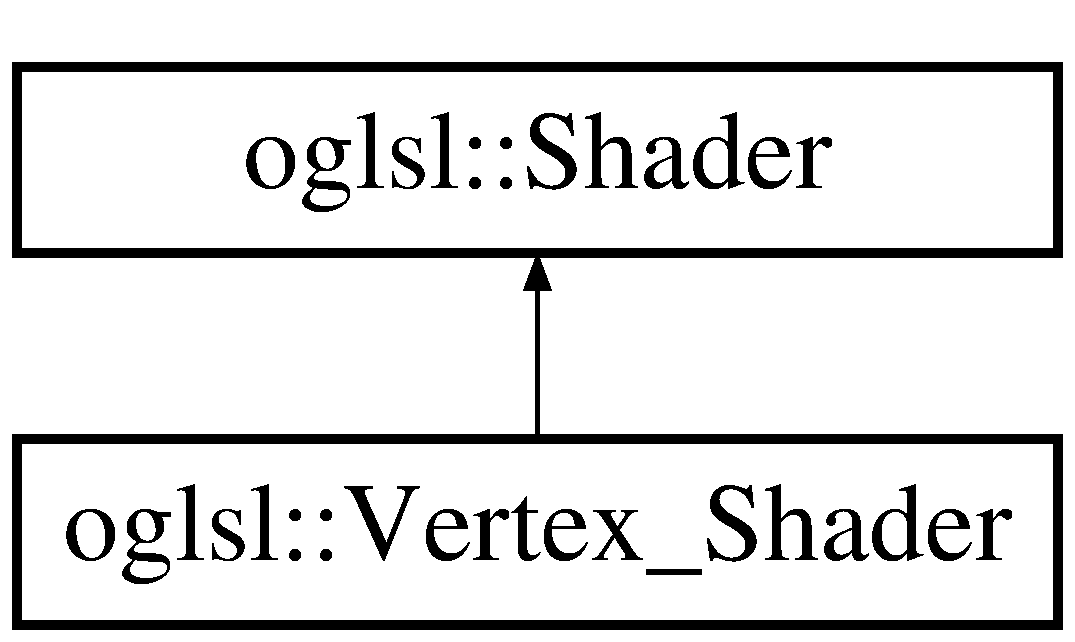
\includegraphics[height=2.000000cm]{classoglsl_1_1_vertex___shader}
\end{center}
\end{figure}
\subsection*{Public Member Functions}
\begin{DoxyCompactItemize}
\item 
\mbox{\hyperlink{classoglsl_1_1_vertex___shader_a73b6548dd06f676a8f7a0882e7f73ad3}{Vertex\+\_\+\+Shader}} (const \mbox{\hyperlink{classoglsl_1_1_shader_1_1_source___code}{Source\+\_\+\+Code}} \&source\+\_\+code)
\end{DoxyCompactItemize}
\subsection*{Additional Inherited Members}


\subsection{Constructor \& Destructor Documentation}
\mbox{\Hypertarget{classoglsl_1_1_vertex___shader_a73b6548dd06f676a8f7a0882e7f73ad3}\label{classoglsl_1_1_vertex___shader_a73b6548dd06f676a8f7a0882e7f73ad3}} 
\index{oglsl\+::\+Vertex\+\_\+\+Shader@{oglsl\+::\+Vertex\+\_\+\+Shader}!Vertex\+\_\+\+Shader@{Vertex\+\_\+\+Shader}}
\index{Vertex\+\_\+\+Shader@{Vertex\+\_\+\+Shader}!oglsl\+::\+Vertex\+\_\+\+Shader@{oglsl\+::\+Vertex\+\_\+\+Shader}}
\subsubsection{\texorpdfstring{Vertex\+\_\+\+Shader()}{Vertex\_Shader()}}
{\footnotesize\ttfamily oglsl\+::\+Vertex\+\_\+\+Shader\+::\+Vertex\+\_\+\+Shader (\begin{DoxyParamCaption}\item[{const \mbox{\hyperlink{classoglsl_1_1_shader_1_1_source___code}{Source\+\_\+\+Code}} \&}]{source\+\_\+code }\end{DoxyParamCaption})\hspace{0.3cm}{\ttfamily [inline]}}



The documentation for this class was generated from the following file\+:\begin{DoxyCompactItemize}
\item 
D\+:/\+Git\+Kraken/3\+D\+Av\+\_\+2/src/\mbox{\hyperlink{_vertex___shader_8hpp}{Vertex\+\_\+\+Shader.\+hpp}}\end{DoxyCompactItemize}

\hypertarget{classoglsl_1_1_view}{}\section{oglsl\+:\+:View Class Reference}
\label{classoglsl_1_1_view}\index{oglsl\+::\+View@{oglsl\+::\+View}}


D\+E\+P\+R\+E\+C\+A\+T\+ED.  




{\ttfamily \#include $<$View.\+hpp$>$}

\subsection*{Public Member Functions}
\begin{DoxyCompactItemize}
\item 
\mbox{\hyperlink{classoglsl_1_1_view_ae7f67b78cdd174449edc93960f29d9f4}{View}} (int width, int height, shared\+\_\+ptr$<$ \mbox{\hyperlink{classoglsl_1_1_scene}{Scene}} $>$ scene)
\begin{DoxyCompactList}\small\item\em Creates a view with the specified dymensions And sets the scene which is going to be rendered. \end{DoxyCompactList}\item 
void \mbox{\hyperlink{classoglsl_1_1_view_ac0b18fc4d2abe1abca6940c55313ef3b}{update}} (\mbox{\hyperlink{classoglsl_1_1_input_a3b21d7328538e661f366af5d6059c197}{Input\+::\+Input\+Data}} input\+\_\+data)
\begin{DoxyCompactList}\small\item\em Applies the imput data to the view Now it\textquotesingle{}s rotating and translating the view. \end{DoxyCompactList}\item 
void \mbox{\hyperlink{classoglsl_1_1_view_a10ea89fc705a2ba2252f673499524bf2}{render}} ()
\begin{DoxyCompactList}\small\item\em Renders every node in the scene. \end{DoxyCompactList}\item 
void \mbox{\hyperlink{classoglsl_1_1_view_a2396337a1db393acefb174e386cde7d1}{resize}} (int width, int height)
\begin{DoxyCompactList}\small\item\em Resizes the view given the window dimensions. \end{DoxyCompactList}\end{DoxyCompactItemize}


\subsection{Detailed Description}
D\+E\+P\+R\+E\+C\+A\+T\+ED. 

\subsection{Constructor \& Destructor Documentation}
\mbox{\Hypertarget{classoglsl_1_1_view_ae7f67b78cdd174449edc93960f29d9f4}\label{classoglsl_1_1_view_ae7f67b78cdd174449edc93960f29d9f4}} 
\index{oglsl\+::\+View@{oglsl\+::\+View}!View@{View}}
\index{View@{View}!oglsl\+::\+View@{oglsl\+::\+View}}
\subsubsection{\texorpdfstring{View()}{View()}}
{\footnotesize\ttfamily example\+::\+View\+::\+View (\begin{DoxyParamCaption}\item[{int}]{width,  }\item[{int}]{height,  }\item[{shared\+\_\+ptr$<$ \mbox{\hyperlink{classoglsl_1_1_scene}{Scene}} $>$}]{scene }\end{DoxyParamCaption})}



Creates a view with the specified dymensions And sets the scene which is going to be rendered. 



\subsection{Member Function Documentation}
\mbox{\Hypertarget{classoglsl_1_1_view_a10ea89fc705a2ba2252f673499524bf2}\label{classoglsl_1_1_view_a10ea89fc705a2ba2252f673499524bf2}} 
\index{oglsl\+::\+View@{oglsl\+::\+View}!render@{render}}
\index{render@{render}!oglsl\+::\+View@{oglsl\+::\+View}}
\subsubsection{\texorpdfstring{render()}{render()}}
{\footnotesize\ttfamily void example\+::\+View\+::render (\begin{DoxyParamCaption}{ }\end{DoxyParamCaption})}



Renders every node in the scene. 

\mbox{\Hypertarget{classoglsl_1_1_view_a2396337a1db393acefb174e386cde7d1}\label{classoglsl_1_1_view_a2396337a1db393acefb174e386cde7d1}} 
\index{oglsl\+::\+View@{oglsl\+::\+View}!resize@{resize}}
\index{resize@{resize}!oglsl\+::\+View@{oglsl\+::\+View}}
\subsubsection{\texorpdfstring{resize()}{resize()}}
{\footnotesize\ttfamily void example\+::\+View\+::resize (\begin{DoxyParamCaption}\item[{int}]{width,  }\item[{int}]{height }\end{DoxyParamCaption})}



Resizes the view given the window dimensions. 


\begin{DoxyParams}{Parameters}
{\em width} & window width \\
\hline
{\em width} & window height \\
\hline
\end{DoxyParams}
\mbox{\Hypertarget{classoglsl_1_1_view_ac0b18fc4d2abe1abca6940c55313ef3b}\label{classoglsl_1_1_view_ac0b18fc4d2abe1abca6940c55313ef3b}} 
\index{oglsl\+::\+View@{oglsl\+::\+View}!update@{update}}
\index{update@{update}!oglsl\+::\+View@{oglsl\+::\+View}}
\subsubsection{\texorpdfstring{update()}{update()}}
{\footnotesize\ttfamily void example\+::\+View\+::update (\begin{DoxyParamCaption}\item[{\mbox{\hyperlink{classoglsl_1_1_input_a3b21d7328538e661f366af5d6059c197}{Input\+::\+Input\+Data}}}]{input\+\_\+data }\end{DoxyParamCaption})}



Applies the imput data to the view Now it\textquotesingle{}s rotating and translating the view. 



The documentation for this class was generated from the following files\+:\begin{DoxyCompactItemize}
\item 
D\+:/\+Git\+Kraken/3\+D\+Av\+\_\+2/src/\mbox{\hyperlink{_view_8hpp}{View.\+hpp}}\item 
D\+:/\+Git\+Kraken/3\+D\+Av\+\_\+2/src/\mbox{\hyperlink{_view_8cpp}{View.\+cpp}}\end{DoxyCompactItemize}

\chapter{File Documentation}
\hypertarget{_camera_8hpp}{}\section{D\+:/\+Git\+Kraken/3\+D\+Av\+\_\+2/src/\+Camera.hpp File Reference}
\label{_camera_8hpp}\index{D\+:/\+Git\+Kraken/3\+D\+Av\+\_\+2/src/\+Camera.\+hpp@{D\+:/\+Git\+Kraken/3\+D\+Av\+\_\+2/src/\+Camera.\+hpp}}
{\ttfamily \#include $<$glm/glm.\+hpp$>$}\newline
{\ttfamily \#include $<$glm/gtc/matrix\+\_\+transform.\+hpp$>$}\newline
{\ttfamily \#include $<$glm/gtc/type\+\_\+ptr.\+hpp$>$}\newline
\subsection*{Classes}
\begin{DoxyCompactItemize}
\item 
class \mbox{\hyperlink{classoglsl_1_1_camera}{oglsl\+::\+Camera}}
\end{DoxyCompactItemize}
\subsection*{Namespaces}
\begin{DoxyCompactItemize}
\item 
 \mbox{\hyperlink{namespaceoglsl}{oglsl}}
\end{DoxyCompactItemize}

\hypertarget{_color___buffer_8hpp}{}\section{D\+:/\+Git\+Kraken/3\+D\+Av\+\_\+2/src/\+Color\+\_\+\+Buffer.hpp File Reference}
\label{_color___buffer_8hpp}\index{D\+:/\+Git\+Kraken/3\+D\+Av\+\_\+2/src/\+Color\+\_\+\+Buffer.\+hpp@{D\+:/\+Git\+Kraken/3\+D\+Av\+\_\+2/src/\+Color\+\_\+\+Buffer.\+hpp}}
\subsection*{Classes}
\begin{DoxyCompactItemize}
\item 
class \mbox{\hyperlink{classoglsl_1_1_color___buffer}{oglsl\+::\+Color\+\_\+\+Buffer}}
\end{DoxyCompactItemize}
\subsection*{Namespaces}
\begin{DoxyCompactItemize}
\item 
 \mbox{\hyperlink{namespaceoglsl}{oglsl}}
\end{DoxyCompactItemize}

\hypertarget{_color___buffer___rgba8888_8hpp}{}\section{D\+:/\+Git\+Kraken/3\+D\+Av\+\_\+2/src/\+Color\+\_\+\+Buffer\+\_\+\+Rgba8888.hpp File Reference}
\label{_color___buffer___rgba8888_8hpp}\index{D\+:/\+Git\+Kraken/3\+D\+Av\+\_\+2/src/\+Color\+\_\+\+Buffer\+\_\+\+Rgba8888.\+hpp@{D\+:/\+Git\+Kraken/3\+D\+Av\+\_\+2/src/\+Color\+\_\+\+Buffer\+\_\+\+Rgba8888.\+hpp}}
{\ttfamily \#include \char`\"{}Color\+\_\+\+Buffer.\+hpp\char`\"{}}\newline
{\ttfamily \#include $<$S\+F\+M\+L/\+Open\+G\+L.\+hpp$>$}\newline
{\ttfamily \#include $<$stdint.\+h$>$}\newline
{\ttfamily \#include $<$vector$>$}\newline
\subsection*{Classes}
\begin{DoxyCompactItemize}
\item 
class \mbox{\hyperlink{classexample_1_1_color___buffer___rgba8888}{example\+::\+Color\+\_\+\+Buffer\+\_\+\+Rgba8888}}
\item 
struct \mbox{\hyperlink{structexample_1_1_color___buffer___rgba8888_1_1_color}{example\+::\+Color\+\_\+\+Buffer\+\_\+\+Rgba8888\+::\+Color}}
\end{DoxyCompactItemize}
\subsection*{Namespaces}
\begin{DoxyCompactItemize}
\item 
 \mbox{\hyperlink{namespaceexample}{example}}
\end{DoxyCompactItemize}

\hypertarget{_cube_8cpp}{}\section{D\+:/\+Git\+Kraken/3\+D\+Av\+\_\+2/src/\+Cube.cpp File Reference}
\label{_cube_8cpp}\index{D\+:/\+Git\+Kraken/3\+D\+Av\+\_\+2/src/\+Cube.\+cpp@{D\+:/\+Git\+Kraken/3\+D\+Av\+\_\+2/src/\+Cube.\+cpp}}
{\ttfamily \#include $<$G\+L/glew.\+h$>$}\newline
{\ttfamily \#include \char`\"{}Cube.\+hpp\char`\"{}}\newline
{\ttfamily \#include $<$S\+F\+M\+L/\+Open\+G\+L.\+hpp$>$}\newline
\subsection*{Namespaces}
\begin{DoxyCompactItemize}
\item 
 \mbox{\hyperlink{namespaceexample}{example}}
\end{DoxyCompactItemize}

\hypertarget{_cube_8hpp}{}\section{D\+:/\+Git\+Kraken/3\+D\+Av\+\_\+2/src/\+Cube.hpp File Reference}
\label{_cube_8hpp}\index{D\+:/\+Git\+Kraken/3\+D\+Av\+\_\+2/src/\+Cube.\+hpp@{D\+:/\+Git\+Kraken/3\+D\+Av\+\_\+2/src/\+Cube.\+hpp}}
{\ttfamily \#include $<$S\+F\+M\+L/\+Open\+G\+L.\+hpp$>$}\newline
\subsection*{Classes}
\begin{DoxyCompactItemize}
\item 
class \mbox{\hyperlink{classexample_1_1_cube}{example\+::\+Cube}}
\end{DoxyCompactItemize}
\subsection*{Namespaces}
\begin{DoxyCompactItemize}
\item 
 \mbox{\hyperlink{namespaceexample}{example}}
\end{DoxyCompactItemize}

\hypertarget{_elevation___mesh_8cpp}{}\section{D\+:/\+Git\+Kraken/3\+D\+Av\+\_\+2/src/\+Elevation\+\_\+\+Mesh.cpp File Reference}
\label{_elevation___mesh_8cpp}\index{D\+:/\+Git\+Kraken/3\+D\+Av\+\_\+2/src/\+Elevation\+\_\+\+Mesh.\+cpp@{D\+:/\+Git\+Kraken/3\+D\+Av\+\_\+2/src/\+Elevation\+\_\+\+Mesh.\+cpp}}
{\ttfamily \#include $<$vector$>$}\newline
{\ttfamily \#include $<$G\+L/glew.\+h$>$}\newline
{\ttfamily \#include \char`\"{}Elevation\+\_\+\+Mesh.\+hpp\char`\"{}}\newline
{\ttfamily \#include $<$S\+F\+M\+L/\+Open\+G\+L.\+hpp$>$}\newline
{\ttfamily \#include \char`\"{}Color\+\_\+\+Buffer\+\_\+\+Rgba8888.\+hpp\char`\"{}}\newline
{\ttfamily \#include $<$targa.\+h$>$}\newline
\subsection*{Namespaces}
\begin{DoxyCompactItemize}
\item 
 \mbox{\hyperlink{namespaceexample}{example}}
\end{DoxyCompactItemize}

\hypertarget{_elevation___mesh_8hpp}{}\section{D\+:/\+Git\+Kraken/3\+D\+Av\+\_\+2/src/\+Elevation\+\_\+\+Mesh.hpp File Reference}
\label{_elevation___mesh_8hpp}\index{D\+:/\+Git\+Kraken/3\+D\+Av\+\_\+2/src/\+Elevation\+\_\+\+Mesh.\+hpp@{D\+:/\+Git\+Kraken/3\+D\+Av\+\_\+2/src/\+Elevation\+\_\+\+Mesh.\+hpp}}
{\ttfamily \#include $<$memory$>$}\newline
{\ttfamily \#include $<$S\+F\+M\+L/\+Open\+G\+L.\+hpp$>$}\newline
{\ttfamily \#include $<$glm/glm.\+hpp$>$}\newline
{\ttfamily \#include \char`\"{}Node.\+hpp\char`\"{}}\newline
{\ttfamily \#include \char`\"{}Shader\+\_\+\+Program.\+hpp\char`\"{}}\newline
\subsection*{Classes}
\begin{DoxyCompactItemize}
\item 
class \mbox{\hyperlink{classoglsl_1_1_elevation___mesh}{oglsl\+::\+Elevation\+\_\+\+Mesh}}
\end{DoxyCompactItemize}
\subsection*{Namespaces}
\begin{DoxyCompactItemize}
\item 
 \mbox{\hyperlink{namespaceoglsl}{oglsl}}
\end{DoxyCompactItemize}
\subsection*{Typedefs}
\begin{DoxyCompactItemize}
\item 
typedef Color\+\_\+\+Buffer\+\_\+\+Rgba8888 \mbox{\hyperlink{namespaceoglsl_a3f3bf2d9553fda1a155d7492ee30d7d0}{oglsl\+::\+Texture}}
\end{DoxyCompactItemize}

\hypertarget{_fragment___shader_8hpp}{}\section{D\+:/\+Git\+Kraken/3\+D\+Av\+\_\+2/src/\+Fragment\+\_\+\+Shader.hpp File Reference}
\label{_fragment___shader_8hpp}\index{D\+:/\+Git\+Kraken/3\+D\+Av\+\_\+2/src/\+Fragment\+\_\+\+Shader.\+hpp@{D\+:/\+Git\+Kraken/3\+D\+Av\+\_\+2/src/\+Fragment\+\_\+\+Shader.\+hpp}}
{\ttfamily \#include \char`\"{}Shader.\+hpp\char`\"{}}\newline
\subsection*{Classes}
\begin{DoxyCompactItemize}
\item 
class \mbox{\hyperlink{classoglsl_1_1_fragment___shader}{oglsl\+::\+Fragment\+\_\+\+Shader}}
\end{DoxyCompactItemize}
\subsection*{Namespaces}
\begin{DoxyCompactItemize}
\item 
 \mbox{\hyperlink{namespaceoglsl}{oglsl}}
\end{DoxyCompactItemize}

\hypertarget{_framebuffer_8cpp}{}\section{D\+:/\+Git\+Kraken/3\+D\+Av\+\_\+2/src/\+Framebuffer.cpp File Reference}
\label{_framebuffer_8cpp}\index{D\+:/\+Git\+Kraken/3\+D\+Av\+\_\+2/src/\+Framebuffer.\+cpp@{D\+:/\+Git\+Kraken/3\+D\+Av\+\_\+2/src/\+Framebuffer.\+cpp}}
{\ttfamily \#include \char`\"{}Framebuffer.\+hpp\char`\"{}}\newline
\subsection*{Namespaces}
\begin{DoxyCompactItemize}
\item 
 \mbox{\hyperlink{namespaceoglsl}{oglsl}}
\end{DoxyCompactItemize}

\hypertarget{_framebuffer_8hpp}{}\section{D\+:/\+Git\+Kraken/3\+D\+Av\+\_\+2/src/\+Framebuffer.hpp File Reference}
\label{_framebuffer_8hpp}\index{D\+:/\+Git\+Kraken/3\+D\+Av\+\_\+2/src/\+Framebuffer.\+hpp@{D\+:/\+Git\+Kraken/3\+D\+Av\+\_\+2/src/\+Framebuffer.\+hpp}}
{\ttfamily \#include $<$memory$>$}\newline
{\ttfamily \#include \char`\"{}Shader\+\_\+\+Program.\+hpp\char`\"{}}\newline
\subsection*{Classes}
\begin{DoxyCompactItemize}
\item 
class \mbox{\hyperlink{classoglsl_1_1_framebuffer}{oglsl\+::\+Framebuffer}}
\begin{DoxyCompactList}\small\item\em Used to render the scene to a framebuffer and apply post processig shaders to it. \end{DoxyCompactList}\end{DoxyCompactItemize}
\subsection*{Namespaces}
\begin{DoxyCompactItemize}
\item 
 \mbox{\hyperlink{namespaceoglsl}{oglsl}}
\end{DoxyCompactItemize}

\hypertarget{_input_8hpp}{}\section{D\+:/\+Git\+Kraken/3\+D\+Av\+\_\+2/src/\+Input.hpp File Reference}
\label{_input_8hpp}\index{D\+:/\+Git\+Kraken/3\+D\+Av\+\_\+2/src/\+Input.\+hpp@{D\+:/\+Git\+Kraken/3\+D\+Av\+\_\+2/src/\+Input.\+hpp}}
{\ttfamily \#include $<$map$>$}\newline
{\ttfamily \#include $<$memory$>$}\newline
{\ttfamily \#include \char`\"{}Variant.\+hpp\char`\"{}}\newline
{\ttfamily \#include $<$S\+F\+M\+L/\+Window.\+hpp$>$}\newline
{\ttfamily \#include $<$S\+F\+M\+L/\+Open\+G\+L.\+hpp$>$}\newline
{\ttfamily \#include $<$glm/glm.\+hpp$>$}\newline
\subsection*{Classes}
\begin{DoxyCompactItemize}
\item 
class \mbox{\hyperlink{classoglsl_1_1_input}{oglsl\+::\+Input}}
\begin{DoxyCompactList}\small\item\em Controls user input. \end{DoxyCompactList}\end{DoxyCompactItemize}
\subsection*{Namespaces}
\begin{DoxyCompactItemize}
\item 
 \mbox{\hyperlink{namespaceoglsl}{oglsl}}
\end{DoxyCompactItemize}

\hypertarget{main_8cpp}{}\section{D\+:/\+Git\+Kraken/3\+D\+Av\+\_\+2/src/main.cpp File Reference}
\label{main_8cpp}\index{D\+:/\+Git\+Kraken/3\+D\+Av\+\_\+2/src/main.\+cpp@{D\+:/\+Git\+Kraken/3\+D\+Av\+\_\+2/src/main.\+cpp}}
{\ttfamily \#include $<$cassert$>$}\newline
{\ttfamily \#include $<$string$>$}\newline
{\ttfamily \#include \char`\"{}my\+Scene.\+hpp\char`\"{}}\newline
{\ttfamily \#include \char`\"{}View.\+hpp\char`\"{}}\newline
{\ttfamily \#include $<$S\+F\+M\+L/\+Window.\+hpp$>$}\newline
{\ttfamily \#include $<$S\+F\+M\+L/\+Open\+G\+L.\+hpp$>$}\newline
{\ttfamily \#include \char`\"{}Input.\+hpp\char`\"{}}\newline
\subsection*{Functions}
\begin{DoxyCompactItemize}
\item 
int \mbox{\hyperlink{main_8cpp_ae66f6b31b5ad750f1fe042a706a4e3d4}{main}} ()
\end{DoxyCompactItemize}


\subsection{Function Documentation}
\mbox{\Hypertarget{main_8cpp_ae66f6b31b5ad750f1fe042a706a4e3d4}\label{main_8cpp_ae66f6b31b5ad750f1fe042a706a4e3d4}} 
\index{main.\+cpp@{main.\+cpp}!main@{main}}
\index{main@{main}!main.\+cpp@{main.\+cpp}}
\subsubsection{\texorpdfstring{main()}{main()}}
{\footnotesize\ttfamily int main (\begin{DoxyParamCaption}{ }\end{DoxyParamCaption})}


\hypertarget{_mesh_8cpp}{}\section{D\+:/\+Git\+Kraken/3\+D\+Av\+\_\+2/src/\+Mesh.cpp File Reference}
\label{_mesh_8cpp}\index{D\+:/\+Git\+Kraken/3\+D\+Av\+\_\+2/src/\+Mesh.\+cpp@{D\+:/\+Git\+Kraken/3\+D\+Av\+\_\+2/src/\+Mesh.\+cpp}}
{\ttfamily \#include \char`\"{}Mesh.\+hpp\char`\"{}}\newline
\subsection*{Namespaces}
\begin{DoxyCompactItemize}
\item 
 \mbox{\hyperlink{namespaceoglsl}{oglsl}}
\end{DoxyCompactItemize}

\hypertarget{_mesh_8hpp}{}\section{D\+:/\+Git\+Kraken/3\+D\+Av\+\_\+2/src/\+Mesh.hpp File Reference}
\label{_mesh_8hpp}\index{D\+:/\+Git\+Kraken/3\+D\+Av\+\_\+2/src/\+Mesh.\+hpp@{D\+:/\+Git\+Kraken/3\+D\+Av\+\_\+2/src/\+Mesh.\+hpp}}
{\ttfamily \#include $<$memory$>$}\newline
{\ttfamily \#include $<$string$>$}\newline
{\ttfamily \#include $<$vector$>$}\newline
{\ttfamily \#include $<$glm/glm.\+hpp$>$}\newline
{\ttfamily \#include $<$glm/gtc/matrix\+\_\+transform.\+hpp$>$}\newline
{\ttfamily \#include $<$glm/gtc/type\+\_\+ptr.\+hpp$>$}\newline
{\ttfamily \#include $<$G\+L/glew.\+h$>$}\newline
{\ttfamily \#include $<$S\+F\+M\+L/\+Open\+G\+L.\+hpp$>$}\newline
{\ttfamily \#include \char`\"{}Color\+\_\+\+Buffer\+\_\+\+Rgba8888.\+hpp\char`\"{}}\newline
{\ttfamily \#include \char`\"{}Shader\+\_\+\+Program.\+hpp\char`\"{}}\newline
\subsection*{Classes}
\begin{DoxyCompactItemize}
\item 
class \mbox{\hyperlink{classoglsl_1_1_mesh}{oglsl\+::\+Mesh}}
\begin{DoxyCompactList}\small\item\em Represents the mesh data of the models. \end{DoxyCompactList}\end{DoxyCompactItemize}
\subsection*{Namespaces}
\begin{DoxyCompactItemize}
\item 
 \mbox{\hyperlink{namespaceoglsl}{oglsl}}
\end{DoxyCompactItemize}

\hypertarget{_model_8cpp}{}\section{D\+:/\+Git\+Kraken/3\+D\+Av\+\_\+2/src/\+Model.cpp File Reference}
\label{_model_8cpp}\index{D\+:/\+Git\+Kraken/3\+D\+Av\+\_\+2/src/\+Model.\+cpp@{D\+:/\+Git\+Kraken/3\+D\+Av\+\_\+2/src/\+Model.\+cpp}}
{\ttfamily \#include \char`\"{}Model.\+hpp\char`\"{}}\newline
{\ttfamily \#include $<$targa.\+h$>$}\newline
\subsection*{Namespaces}
\begin{DoxyCompactItemize}
\item 
 \mbox{\hyperlink{namespaceoglsl}{oglsl}}
\end{DoxyCompactItemize}

\hypertarget{_model_8hpp}{}\section{D\+:/\+Git\+Kraken/3\+D\+Av\+\_\+2/src/\+Model.hpp File Reference}
\label{_model_8hpp}\index{D\+:/\+Git\+Kraken/3\+D\+Av\+\_\+2/src/\+Model.\+hpp@{D\+:/\+Git\+Kraken/3\+D\+Av\+\_\+2/src/\+Model.\+hpp}}
{\ttfamily \#include $<$iostream$>$}\newline
{\ttfamily \#include $<$scene.\+h$>$}\newline
{\ttfamily \#include $<$Importer.\+hpp$>$}\newline
{\ttfamily \#include $<$postprocess.\+h$>$}\newline
{\ttfamily \#include \char`\"{}Node.\+hpp\char`\"{}}\newline
{\ttfamily \#include \char`\"{}Mesh.\+hpp\char`\"{}}\newline
\subsection*{Classes}
\begin{DoxyCompactItemize}
\item 
class \mbox{\hyperlink{classexample_1_1_model}{example\+::\+Model}}
\end{DoxyCompactItemize}
\subsection*{Namespaces}
\begin{DoxyCompactItemize}
\item 
 \mbox{\hyperlink{namespaceexample}{example}}
\end{DoxyCompactItemize}

\hypertarget{my_scene_8cpp}{}\section{D\+:/\+Git\+Kraken/3\+D\+Av\+\_\+2/src/my\+Scene.cpp File Reference}
\label{my_scene_8cpp}\index{D\+:/\+Git\+Kraken/3\+D\+Av\+\_\+2/src/my\+Scene.\+cpp@{D\+:/\+Git\+Kraken/3\+D\+Av\+\_\+2/src/my\+Scene.\+cpp}}
{\ttfamily \#include \char`\"{}my\+Scene.\+hpp\char`\"{}}\newline
{\ttfamily \#include $<$glm/glm.\+hpp$>$}\newline
{\ttfamily \#include $<$glm/gtc/matrix\+\_\+transform.\+hpp$>$}\newline
{\ttfamily \#include $<$glm/gtc/type\+\_\+ptr.\+hpp$>$}\newline
\subsection*{Namespaces}
\begin{DoxyCompactItemize}
\item 
 \mbox{\hyperlink{namespaceoglsl}{oglsl}}
\end{DoxyCompactItemize}

\hypertarget{my_scene_8hpp}{}\section{D\+:/\+Git\+Kraken/3\+D\+Av\+\_\+2/src/my\+Scene.hpp File Reference}
\label{my_scene_8hpp}\index{D\+:/\+Git\+Kraken/3\+D\+Av\+\_\+2/src/my\+Scene.\+hpp@{D\+:/\+Git\+Kraken/3\+D\+Av\+\_\+2/src/my\+Scene.\+hpp}}
{\ttfamily \#include \char`\"{}Scene.\+hpp\char`\"{}}\newline
{\ttfamily \#include \char`\"{}Elevation\+\_\+\+Mesh.\+hpp\char`\"{}}\newline
{\ttfamily \#include \char`\"{}Model.\+hpp\char`\"{}}\newline
\subsection*{Classes}
\begin{DoxyCompactItemize}
\item 
class \mbox{\hyperlink{classoglsl_1_1my_scene}{oglsl\+::my\+Scene}}
\begin{DoxyCompactList}\small\item\em Custom \mbox{\hyperlink{classoglsl_1_1_scene}{Scene}} for this specific example. \end{DoxyCompactList}\end{DoxyCompactItemize}
\subsection*{Namespaces}
\begin{DoxyCompactItemize}
\item 
 \mbox{\hyperlink{namespaceoglsl}{oglsl}}
\end{DoxyCompactItemize}

\hypertarget{_node_8hpp}{}\section{D\+:/\+Git\+Kraken/3\+D\+Av\+\_\+2/src/\+Node.hpp File Reference}
\label{_node_8hpp}\index{D\+:/\+Git\+Kraken/3\+D\+Av\+\_\+2/src/\+Node.\+hpp@{D\+:/\+Git\+Kraken/3\+D\+Av\+\_\+2/src/\+Node.\+hpp}}
\subsection*{Classes}
\begin{DoxyCompactItemize}
\item 
class \mbox{\hyperlink{classexample_1_1_node}{example\+::\+Node}}
\end{DoxyCompactItemize}
\subsection*{Namespaces}
\begin{DoxyCompactItemize}
\item 
 \mbox{\hyperlink{namespaceexample}{example}}
\end{DoxyCompactItemize}

\hypertarget{_scene_8cpp}{}\section{D\+:/\+Git\+Kraken/3\+D\+Av\+\_\+2/src/\+Scene.cpp File Reference}
\label{_scene_8cpp}\index{D\+:/\+Git\+Kraken/3\+D\+Av\+\_\+2/src/\+Scene.\+cpp@{D\+:/\+Git\+Kraken/3\+D\+Av\+\_\+2/src/\+Scene.\+cpp}}
{\ttfamily \#include \char`\"{}Scene.\+hpp\char`\"{}}\newline
\subsection*{Namespaces}
\begin{DoxyCompactItemize}
\item 
 \mbox{\hyperlink{namespaceoglsl}{oglsl}}
\end{DoxyCompactItemize}

\hypertarget{_scene_8hpp}{}\section{D\+:/\+Git\+Kraken/3\+D\+Av\+\_\+2/src/\+Scene.hpp File Reference}
\label{_scene_8hpp}\index{D\+:/\+Git\+Kraken/3\+D\+Av\+\_\+2/src/\+Scene.\+hpp@{D\+:/\+Git\+Kraken/3\+D\+Av\+\_\+2/src/\+Scene.\+hpp}}
{\ttfamily \#include $<$map$>$}\newline
{\ttfamily \#include $<$memory$>$}\newline
{\ttfamily \#include $<$vector$>$}\newline
{\ttfamily \#include \char`\"{}Node.\+hpp\char`\"{}}\newline
{\ttfamily \#include \char`\"{}Camera.\+hpp\char`\"{}}\newline
{\ttfamily \#include \char`\"{}Skybox.\+hpp\char`\"{}}\newline
{\ttfamily \#include \char`\"{}Shader\+\_\+\+Program.\+hpp\char`\"{}}\newline
{\ttfamily \#include \char`\"{}Vertex\+\_\+\+Shader.\+hpp\char`\"{}}\newline
{\ttfamily \#include \char`\"{}Fragment\+\_\+\+Shader.\+hpp\char`\"{}}\newline
{\ttfamily \#include \char`\"{}Input.\+hpp\char`\"{}}\newline
\subsection*{Classes}
\begin{DoxyCompactItemize}
\item 
class \mbox{\hyperlink{classoglsl_1_1_scene}{oglsl\+::\+Scene}}
\end{DoxyCompactItemize}
\subsection*{Namespaces}
\begin{DoxyCompactItemize}
\item 
 \mbox{\hyperlink{namespaceoglsl}{oglsl}}
\end{DoxyCompactItemize}

\hypertarget{_shader_8cpp}{}\section{D\+:/\+Git\+Kraken/3\+D\+Av\+\_\+2/src/\+Shader.cpp File Reference}
\label{_shader_8cpp}\index{D\+:/\+Git\+Kraken/3\+D\+Av\+\_\+2/src/\+Shader.\+cpp@{D\+:/\+Git\+Kraken/3\+D\+Av\+\_\+2/src/\+Shader.\+cpp}}
{\ttfamily \#include $<$cassert$>$}\newline
{\ttfamily \#include $<$fstream$>$}\newline
{\ttfamily \#include $<$iostream$>$}\newline
{\ttfamily \#include \char`\"{}Shader.\+hpp\char`\"{}}\newline
\subsection*{Namespaces}
\begin{DoxyCompactItemize}
\item 
 \mbox{\hyperlink{namespaceoglsl}{oglsl}}
\end{DoxyCompactItemize}

\hypertarget{_shader_8hpp}{}\section{D\+:/\+Git\+Kraken/3\+D\+Av\+\_\+2/src/\+Shader.hpp File Reference}
\label{_shader_8hpp}\index{D\+:/\+Git\+Kraken/3\+D\+Av\+\_\+2/src/\+Shader.\+hpp@{D\+:/\+Git\+Kraken/3\+D\+Av\+\_\+2/src/\+Shader.\+hpp}}
{\ttfamily \#include $<$string$>$}\newline
{\ttfamily \#include $<$G\+L/glew.\+h$>$}\newline
\subsection*{Classes}
\begin{DoxyCompactItemize}
\item 
class \mbox{\hyperlink{classoglsl_1_1_shader}{oglsl\+::\+Shader}}
\item 
class \mbox{\hyperlink{classoglsl_1_1_shader_1_1_source___code}{oglsl\+::\+Shader\+::\+Source\+\_\+\+Code}}
\end{DoxyCompactItemize}
\subsection*{Namespaces}
\begin{DoxyCompactItemize}
\item 
 \mbox{\hyperlink{namespaceoglsl}{oglsl}}
\end{DoxyCompactItemize}

\hypertarget{_shader___program_8cpp}{}\section{D\+:/\+Git\+Kraken/3\+D\+Av\+\_\+2/src/\+Shader\+\_\+\+Program.cpp File Reference}
\label{_shader___program_8cpp}\index{D\+:/\+Git\+Kraken/3\+D\+Av\+\_\+2/src/\+Shader\+\_\+\+Program.\+cpp@{D\+:/\+Git\+Kraken/3\+D\+Av\+\_\+2/src/\+Shader\+\_\+\+Program.\+cpp}}
{\ttfamily \#include \char`\"{}Shader\+\_\+\+Program.\+hpp\char`\"{}}\newline
\subsection*{Namespaces}
\begin{DoxyCompactItemize}
\item 
 \mbox{\hyperlink{namespaceoglsl}{oglsl}}
\end{DoxyCompactItemize}

\hypertarget{_shader___program_8hpp}{}\section{D\+:/\+Git\+Kraken/3\+D\+Av\+\_\+2/src/\+Shader\+\_\+\+Program.hpp File Reference}
\label{_shader___program_8hpp}\index{D\+:/\+Git\+Kraken/3\+D\+Av\+\_\+2/src/\+Shader\+\_\+\+Program.\+hpp@{D\+:/\+Git\+Kraken/3\+D\+Av\+\_\+2/src/\+Shader\+\_\+\+Program.\+hpp}}
{\ttfamily \#include $<$cassert$>$}\newline
{\ttfamily \#include \char`\"{}Shader.\+hpp\char`\"{}}\newline
{\ttfamily \#include $<$glm/glm.\+hpp$>$}\newline
{\ttfamily \#include $<$glm/gtc/matrix\+\_\+transform.\+hpp$>$}\newline
{\ttfamily \#include $<$glm/gtc/type\+\_\+ptr.\+hpp$>$}\newline
\subsection*{Classes}
\begin{DoxyCompactItemize}
\item 
class \mbox{\hyperlink{classoglsl_1_1_shader___program}{oglsl\+::\+Shader\+\_\+\+Program}}
\end{DoxyCompactItemize}
\subsection*{Namespaces}
\begin{DoxyCompactItemize}
\item 
 \mbox{\hyperlink{namespaceoglsl}{oglsl}}
\end{DoxyCompactItemize}

\hypertarget{_skybox_8cpp}{}\section{D\+:/\+Git\+Kraken/3\+D\+Av\+\_\+2/src/\+Skybox.cpp File Reference}
\label{_skybox_8cpp}\index{D\+:/\+Git\+Kraken/3\+D\+Av\+\_\+2/src/\+Skybox.\+cpp@{D\+:/\+Git\+Kraken/3\+D\+Av\+\_\+2/src/\+Skybox.\+cpp}}
{\ttfamily \#include $<$cassert$>$}\newline
{\ttfamily \#include $<$G\+L/glew.\+h$>$}\newline
{\ttfamily \#include \char`\"{}Skybox.\+hpp\char`\"{}}\newline
{\ttfamily \#include $<$S\+F\+M\+L/\+Open\+G\+L.\+hpp$>$}\newline
{\ttfamily \#include \char`\"{}Vertex\+\_\+\+Shader.\+hpp\char`\"{}}\newline
{\ttfamily \#include \char`\"{}Fragment\+\_\+\+Shader.\+hpp\char`\"{}}\newline
\subsection*{Namespaces}
\begin{DoxyCompactItemize}
\item 
 \mbox{\hyperlink{namespaceoglsl}{oglsl}}
\end{DoxyCompactItemize}

\hypertarget{_skybox_8hpp}{}\section{D\+:/\+Git\+Kraken/3\+D\+Av\+\_\+2/src/\+Skybox.hpp File Reference}
\label{_skybox_8hpp}\index{D\+:/\+Git\+Kraken/3\+D\+Av\+\_\+2/src/\+Skybox.\+hpp@{D\+:/\+Git\+Kraken/3\+D\+Av\+\_\+2/src/\+Skybox.\+hpp}}
{\ttfamily \#include $<$vector$>$}\newline
{\ttfamily \#include $<$memory$>$}\newline
{\ttfamily \#include \char`\"{}Camera.\+hpp\char`\"{}}\newline
{\ttfamily \#include \char`\"{}Texture\+\_\+\+Cube.\+hpp\char`\"{}}\newline
{\ttfamily \#include \char`\"{}Shader\+\_\+\+Program.\+hpp\char`\"{}}\newline
\subsection*{Classes}
\begin{DoxyCompactItemize}
\item 
class \mbox{\hyperlink{classoglsl_1_1_skybox}{oglsl\+::\+Skybox}}
\end{DoxyCompactItemize}
\subsection*{Namespaces}
\begin{DoxyCompactItemize}
\item 
 \mbox{\hyperlink{namespaceoglsl}{oglsl}}
\end{DoxyCompactItemize}

\hypertarget{_texture___cube_8cpp}{}\section{D\+:/\+Git\+Kraken/3\+D\+Av\+\_\+2/src/\+Texture\+\_\+\+Cube.cpp File Reference}
\label{_texture___cube_8cpp}\index{D\+:/\+Git\+Kraken/3\+D\+Av\+\_\+2/src/\+Texture\+\_\+\+Cube.\+cpp@{D\+:/\+Git\+Kraken/3\+D\+Av\+\_\+2/src/\+Texture\+\_\+\+Cube.\+cpp}}
{\ttfamily \#include $<$vector$>$}\newline
{\ttfamily \#include \char`\"{}Texture\+\_\+\+Cube.\+hpp\char`\"{}}\newline
{\ttfamily \#include $<$targa.\+h$>$}\newline
\subsection*{Namespaces}
\begin{DoxyCompactItemize}
\item 
 \mbox{\hyperlink{namespaceoglsl}{oglsl}}
\end{DoxyCompactItemize}
\subsection*{Typedefs}
\begin{DoxyCompactItemize}
\item 
typedef Color\+\_\+\+Buffer\+\_\+\+Rgba8888 \mbox{\hyperlink{namespaceoglsl_a54a481d3b94c4faefeb16560e4b85a34}{oglsl\+::\+Buffer}}
\end{DoxyCompactItemize}

\hypertarget{_texture___cube_8hpp}{}\section{D\+:/\+Git\+Kraken/3\+D\+Av\+\_\+2/src/\+Texture\+\_\+\+Cube.hpp File Reference}
\label{_texture___cube_8hpp}\index{D\+:/\+Git\+Kraken/3\+D\+Av\+\_\+2/src/\+Texture\+\_\+\+Cube.\+hpp@{D\+:/\+Git\+Kraken/3\+D\+Av\+\_\+2/src/\+Texture\+\_\+\+Cube.\+hpp}}
{\ttfamily \#include $<$memory$>$}\newline
{\ttfamily \#include $<$string$>$}\newline
{\ttfamily \#include $<$G\+L/glew.\+h$>$}\newline
{\ttfamily \#include $<$S\+F\+M\+L/\+Open\+G\+L.\+hpp$>$}\newline
{\ttfamily \#include \char`\"{}Color\+\_\+\+Buffer\+\_\+\+Rgba8888.\+hpp\char`\"{}}\newline
\subsection*{Classes}
\begin{DoxyCompactItemize}
\item 
class \mbox{\hyperlink{classoglsl_1_1_texture___cube}{oglsl\+::\+Texture\+\_\+\+Cube}}
\end{DoxyCompactItemize}
\subsection*{Namespaces}
\begin{DoxyCompactItemize}
\item 
 \mbox{\hyperlink{namespaceoglsl}{oglsl}}
\end{DoxyCompactItemize}

\hypertarget{_variant_8hpp}{}\section{D\+:/\+Git\+Kraken/3\+D\+Av\+\_\+2/src/\+Variant.hpp File Reference}
\label{_variant_8hpp}\index{D\+:/\+Git\+Kraken/3\+D\+Av\+\_\+2/src/\+Variant.\+hpp@{D\+:/\+Git\+Kraken/3\+D\+Av\+\_\+2/src/\+Variant.\+hpp}}
{\ttfamily \#include $<$string$>$}\newline
\subsection*{Classes}
\begin{DoxyCompactItemize}
\item 
class \mbox{\hyperlink{classoglsl_1_1_variant}{oglsl\+::\+Variant}}
\end{DoxyCompactItemize}
\subsection*{Namespaces}
\begin{DoxyCompactItemize}
\item 
 \mbox{\hyperlink{namespaceoglsl}{oglsl}}
\end{DoxyCompactItemize}

\hypertarget{_vertex___shader_8hpp}{}\section{D\+:/\+Git\+Kraken/3\+D\+Av\+\_\+2/src/\+Vertex\+\_\+\+Shader.hpp File Reference}
\label{_vertex___shader_8hpp}\index{D\+:/\+Git\+Kraken/3\+D\+Av\+\_\+2/src/\+Vertex\+\_\+\+Shader.\+hpp@{D\+:/\+Git\+Kraken/3\+D\+Av\+\_\+2/src/\+Vertex\+\_\+\+Shader.\+hpp}}
{\ttfamily \#include \char`\"{}Shader.\+hpp\char`\"{}}\newline
\subsection*{Classes}
\begin{DoxyCompactItemize}
\item 
class \mbox{\hyperlink{classoglsl_1_1_vertex___shader}{oglsl\+::\+Vertex\+\_\+\+Shader}}
\end{DoxyCompactItemize}
\subsection*{Namespaces}
\begin{DoxyCompactItemize}
\item 
 \mbox{\hyperlink{namespaceoglsl}{oglsl}}
\end{DoxyCompactItemize}

\hypertarget{_view_8cpp}{}\section{D\+:/\+Git\+Kraken/3\+D\+Av\+\_\+2/src/\+View.cpp File Reference}
\label{_view_8cpp}\index{D\+:/\+Git\+Kraken/3\+D\+Av\+\_\+2/src/\+View.\+cpp@{D\+:/\+Git\+Kraken/3\+D\+Av\+\_\+2/src/\+View.\+cpp}}
{\ttfamily \#include \char`\"{}View.\+hpp\char`\"{}}\newline
{\ttfamily \#include $<$iostream$>$}\newline
{\ttfamily \#include $<$cassert$>$}\newline
{\ttfamily \#include $<$glm/glm.\+hpp$>$}\newline
{\ttfamily \#include $<$glm/gtc/matrix\+\_\+transform.\+hpp$>$}\newline
{\ttfamily \#include $<$glm/gtc/type\+\_\+ptr.\+hpp$>$}\newline
\subsection*{Namespaces}
\begin{DoxyCompactItemize}
\item 
 \mbox{\hyperlink{namespaceexample}{example}}
\end{DoxyCompactItemize}

\hypertarget{_view_8hpp}{}\section{D\+:/\+Git\+Kraken/3\+D\+Av\+\_\+2/src/\+View.hpp File Reference}
\label{_view_8hpp}\index{D\+:/\+Git\+Kraken/3\+D\+Av\+\_\+2/src/\+View.\+hpp@{D\+:/\+Git\+Kraken/3\+D\+Av\+\_\+2/src/\+View.\+hpp}}
{\ttfamily \#include $<$string$>$}\newline
{\ttfamily \#include $<$G\+L/glew.\+h$>$}\newline
{\ttfamily \#include \char`\"{}Cube.\+hpp\char`\"{}}\newline
{\ttfamily \#include \char`\"{}Scene.\+hpp\char`\"{}}\newline
{\ttfamily \#include \char`\"{}Input.\+hpp\char`\"{}}\newline
\subsection*{Classes}
\begin{DoxyCompactItemize}
\item 
class \mbox{\hyperlink{classoglsl_1_1_view}{oglsl\+::\+View}}
\begin{DoxyCompactList}\small\item\em D\+E\+P\+R\+E\+C\+A\+T\+ED. \end{DoxyCompactList}\end{DoxyCompactItemize}
\subsection*{Namespaces}
\begin{DoxyCompactItemize}
\item 
 \mbox{\hyperlink{namespaceoglsl}{oglsl}}
\end{DoxyCompactItemize}

%--- End generated contents ---

% Index
\backmatter
\newpage
\phantomsection
\clearemptydoublepage
\addcontentsline{toc}{chapter}{Index}
\printindex

\end{document}
